\documentclass[12pt]{article}
\usepackage[margin=1in]{geometry} 
\usepackage{amsmath,amsthm,amssymb,amsfonts}
\usepackage{graphicx}
\usepackage{listings}
\usepackage{enumitem}
\usepackage{amsmath}
\usepackage{tikz}

\newcommand{\N}{\mathbb{N}}
\newcommand{\Z}{\mathbb{Z}}
 
\newenvironment{problem}[2][Problem]{\begin{trivlist}
\item[\hskip \labelsep {\bfseries #1}\hskip \labelsep {\bfseries #2.}]}{\end{trivlist}}
\setlength{\parskip}{1em}

\begin{document}
\title{COMP.3040 Homework 1}

\maketitle

\begin{problem}{1.3}
\end{problem}

\tikzset{every picture/.style={line width=0.75pt}} %set default line width to 0.75pt        

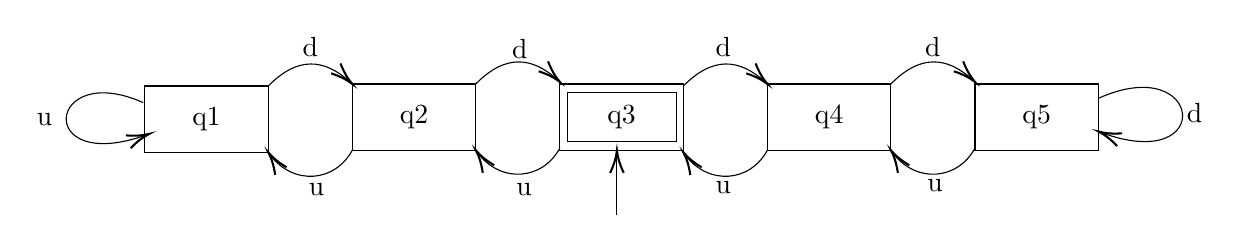
\begin{tikzpicture}[x=0.75pt,y=0.75pt,yscale=-1,xscale=1]
%uncomment if require: \path (0,177); %set diagram left start at 0, and has height of 177

%Shape: Rectangle [id:dp8403825739642081] 
\draw   (96,84) -- (155.5,84) -- (155.5,115.91) -- (96,115.91) -- cycle ;
%Shape: Rectangle [id:dp3255366457093698] 
\draw   (196,83) -- (255.5,83) -- (255.5,114.91) -- (196,114.91) -- cycle ;
%Shape: Rectangle [id:dp42453654604612523] 
\draw   (296,83) -- (355.5,83) -- (355.5,114.91) -- (296,114.91) -- cycle ;
%Shape: Rectangle [id:dp9694573772398549] 
\draw   (396,83) -- (455.5,83) -- (455.5,114.91) -- (396,114.91) -- cycle ;
%Curve Lines [id:da005580042369051963] 
\draw    (555.5,89.91) .. controls (605.99,67.14) and (612.38,126.69) .. (557.19,106.54) ;
\draw [shift={(555.5,105.91)}, rotate = 381.1] [color={rgb, 255:red, 0; green, 0; blue, 0 }  ][line width=0.75]    (10.93,-3.29) .. controls (6.95,-1.4) and (3.31,-0.3) .. (0,0) .. controls (3.31,0.3) and (6.95,1.4) .. (10.93,3.29)   ;

%Shape: Rectangle [id:dp7389555063338928] 
\draw   (496,83) -- (555.5,83) -- (555.5,114.91) -- (496,114.91) -- cycle ;
%Curve Lines [id:da38604976277341696] 
\draw    (155.5,84) .. controls (169.78,69.52) and (182.39,70.88) .. (194.67,81.78) ;
\draw [shift={(196,83)}, rotate = 223.38] [color={rgb, 255:red, 0; green, 0; blue, 0 }  ][line width=0.75]    (10.93,-3.29) .. controls (6.95,-1.4) and (3.31,-0.3) .. (0,0) .. controls (3.31,0.3) and (6.95,1.4) .. (10.93,3.29)   ;

%Curve Lines [id:da37114515706489826] 
\draw    (156.67,117.53) .. controls (167.75,131.91) and (187.6,130.44) .. (196,114.91) ;

\draw [shift={(155.5,115.91)}, rotate = 56.14] [color={rgb, 255:red, 0; green, 0; blue, 0 }  ][line width=0.75]    (10.93,-3.29) .. controls (6.95,-1.4) and (3.31,-0.3) .. (0,0) .. controls (3.31,0.3) and (6.95,1.4) .. (10.93,3.29)   ;
%Curve Lines [id:da29829675615150886] 
\draw    (255.5,83) .. controls (269.78,68.52) and (282.39,69.88) .. (294.67,80.78) ;
\draw [shift={(296,82)}, rotate = 223.38] [color={rgb, 255:red, 0; green, 0; blue, 0 }  ][line width=0.75]    (10.93,-3.29) .. controls (6.95,-1.4) and (3.31,-0.3) .. (0,0) .. controls (3.31,0.3) and (6.95,1.4) .. (10.93,3.29)   ;

%Curve Lines [id:da7647265012844668] 
\draw    (256.67,116.53) .. controls (267.75,130.91) and (287.6,129.44) .. (296,113.91) ;

\draw [shift={(255.5,114.91)}, rotate = 56.14] [color={rgb, 255:red, 0; green, 0; blue, 0 }  ][line width=0.75]    (10.93,-3.29) .. controls (6.95,-1.4) and (3.31,-0.3) .. (0,0) .. controls (3.31,0.3) and (6.95,1.4) .. (10.93,3.29)   ;
%Curve Lines [id:da2248036357180505] 
\draw    (355.5,84) .. controls (369.78,69.52) and (382.39,70.88) .. (394.67,81.78) ;
\draw [shift={(396,83)}, rotate = 223.38] [color={rgb, 255:red, 0; green, 0; blue, 0 }  ][line width=0.75]    (10.93,-3.29) .. controls (6.95,-1.4) and (3.31,-0.3) .. (0,0) .. controls (3.31,0.3) and (6.95,1.4) .. (10.93,3.29)   ;

%Curve Lines [id:da4842069080288556] 
\draw    (356.67,117.53) .. controls (367.75,131.91) and (387.6,130.44) .. (396,114.91) ;

\draw [shift={(355.5,115.91)}, rotate = 56.14] [color={rgb, 255:red, 0; green, 0; blue, 0 }  ][line width=0.75]    (10.93,-3.29) .. controls (6.95,-1.4) and (3.31,-0.3) .. (0,0) .. controls (3.31,0.3) and (6.95,1.4) .. (10.93,3.29)   ;
%Curve Lines [id:da8401937495832272] 
\draw    (455.5,83) .. controls (469.78,68.52) and (482.39,69.88) .. (494.67,80.78) ;
\draw [shift={(496,82)}, rotate = 223.38] [color={rgb, 255:red, 0; green, 0; blue, 0 }  ][line width=0.75]    (10.93,-3.29) .. controls (6.95,-1.4) and (3.31,-0.3) .. (0,0) .. controls (3.31,0.3) and (6.95,1.4) .. (10.93,3.29)   ;

%Curve Lines [id:da42375047189549053] 
\draw    (456.67,116.53) .. controls (467.75,130.91) and (487.6,129.44) .. (496,113.91) ;

\draw [shift={(455.5,114.91)}, rotate = 56.14] [color={rgb, 255:red, 0; green, 0; blue, 0 }  ][line width=0.75]    (10.93,-3.29) .. controls (6.95,-1.4) and (3.31,-0.3) .. (0,0) .. controls (3.31,0.3) and (6.95,1.4) .. (10.93,3.29)   ;
%Straight Lines [id:da7691005954621644] 
\draw    (323.5,116.91) -- (323.5,145.91) ;

\draw [shift={(323.5,114.91)}, rotate = 90] [color={rgb, 255:red, 0; green, 0; blue, 0 }  ][line width=0.75]    (10.93,-3.29) .. controls (6.95,-1.4) and (3.31,-0.3) .. (0,0) .. controls (3.31,0.3) and (6.95,1.4) .. (10.93,3.29)   ;
%Curve Lines [id:da5109631051731078] 
\draw    (95.3,92) .. controls (48.77,71.21) and (42.42,126.87) .. (96.64,107.61) ;
\draw [shift={(98.3,107)}, rotate = 519.44] [color={rgb, 255:red, 0; green, 0; blue, 0 }  ][line width=0.75]    (10.93,-3.29) .. controls (6.95,-1.4) and (3.31,-0.3) .. (0,0) .. controls (3.31,0.3) and (6.95,1.4) .. (10.93,3.29)   ;

%Shape: Rectangle [id:dp9416865331956659] 
\draw   (299.5,87) -- (352,87) -- (352,110.91) -- (299.5,110.91) -- cycle ;

% Text Node
\draw (125.75,99.95) node  [align=left] {q1};
% Text Node
\draw (225.75,98.95) node  [align=left] {q2};
% Text Node
\draw (325.75,98.95) node  [align=left] {q3};
% Text Node
\draw (425.75,98.95) node  [align=left] {q4};
% Text Node
\draw (525.75,98.95) node  [align=left] {q5};
% Text Node
\draw (47.75,99.95) node  [align=left] {u};
% Text Node
\draw (178.75,133.95) node  [align=left] {u};
% Text Node
\draw (278.75,133.95) node  [align=left] {u};
% Text Node
\draw (374.75,132.95) node  [align=left] {u};
% Text Node
\draw (476.75,131.95) node  [align=left] {u};
% Text Node
\draw (175.75,64.95) node  [align=left] {d};
% Text Node
\draw (276.75,65.95) node  [align=left] {d};
% Text Node
\draw (374.75,64.95) node  [align=left] {d};
% Text Node
\draw (475.75,64.95) node  [align=left] {d};
% Text Node
\draw (601.75,96.95) node  [align=left] {d};

\end{tikzpicture}

\begin{problem}{1.4}
\end{problem}
\begin{enumerate}
	\item[(a)]
		$L_1$ = $\{$w $|$ w has at least three a's $\}$ = $\{ \: \{\varepsilon, a, aa, aaa\}, \{a, b\},\delta_a, \varepsilon, aaa\}$	\\
		$\delta_a = 
			\begin{array}{ c|c|c }
				 & a & b\\
				\hline
				\varepsilon & a & \varepsilon\\
				\hline
				a & aa & a\\
				\hline
				aa & aaa & aa\\
				\hline
				aaa & aaa & aaa
			\end{array}$\\

		$L_2$ = $\{$w $|$ w has at least two b's $\}$	 = $\{ \: \{\varepsilon, b, bb\}, \{a, b\}, \delta_b,\varepsilon, bb\}$	\\
		$\delta_b = 
		\begin{array}{ c|c|c }
			 & b & a\\
			\hline
			\varepsilon & b & \varepsilon\\
			\hline
			b & bb & b\\
			\hline
			bb & bb & bb
		\end{array}$\\

		Combining $L_1$ and $L_2$:	

		\tikzset{every picture/.style={line width=0.75pt}} %set default line width to 0.75pt        
		
		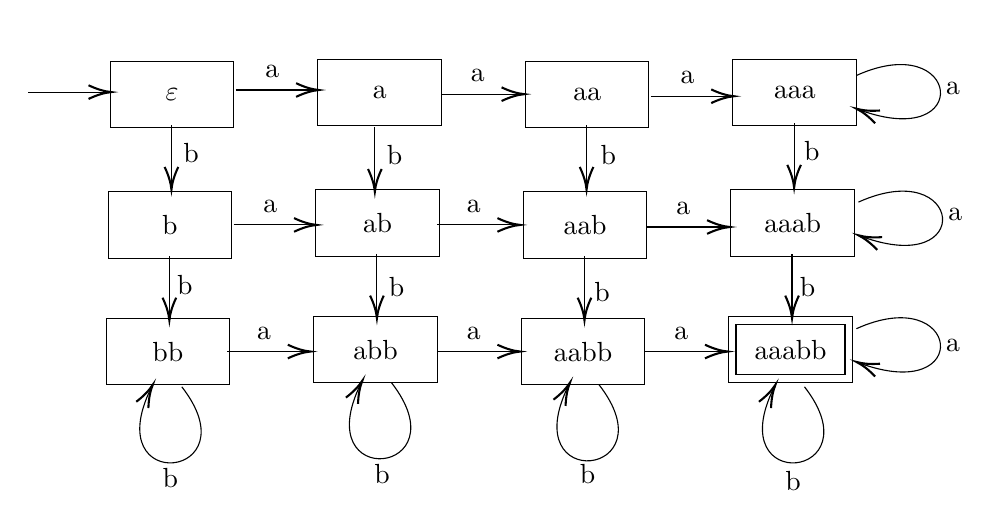
\begin{tikzpicture}[x=0.75pt,y=0.75pt,yscale=-1,xscale=1]
		%uncomment if require: \path (0,376.90625); %set diagram left start at 0, and has height of 376.90625
		
		%Shape: Rectangle [id:dp670868720534658] 
		\draw   (238,51) -- (297.5,51) -- (297.5,82.91) -- (238,82.91) -- cycle ;
		%Straight Lines [id:da34554245232336944] 
		\draw    (198.5,65.91) -- (236.5,65.91) ;
		\draw [shift={(238.5,65.91)}, rotate = 180] [color={rgb, 255:red, 0; green, 0; blue, 0 }  ][line width=0.75]    (10.93,-3.29) .. controls (6.95,-1.4) and (3.31,-0.3) .. (0,0) .. controls (3.31,0.3) and (6.95,1.4) .. (10.93,3.29)   ;
		
		%Straight Lines [id:da2654375756440992] 
		\draw    (267.5,81.91) -- (267.5,110.91) ;
		\draw [shift={(267.5,112.91)}, rotate = 270] [color={rgb, 255:red, 0; green, 0; blue, 0 }  ][line width=0.75]    (10.93,-3.29) .. controls (6.95,-1.4) and (3.31,-0.3) .. (0,0) .. controls (3.31,0.3) and (6.95,1.4) .. (10.93,3.29)   ;
		
		%Shape: Rectangle [id:dp8432284740301497] 
		\draw   (338,50) -- (397.5,50) -- (397.5,81.91) -- (338,81.91) -- cycle ;
		%Straight Lines [id:da49954974135501296] 
		\draw    (298.5,64.91) -- (336.5,64.91) ;
		\draw [shift={(338.5,64.91)}, rotate = 180] [color={rgb, 255:red, 0; green, 0; blue, 0 }  ][line width=0.75]    (10.93,-3.29) .. controls (6.95,-1.4) and (3.31,-0.3) .. (0,0) .. controls (3.31,0.3) and (6.95,1.4) .. (10.93,3.29)   ;
		
		%Shape: Rectangle [id:dp33590878812179636] 
		\draw   (237,114) -- (296.5,114) -- (296.5,145.91) -- (237,145.91) -- cycle ;
		%Straight Lines [id:da6806853469350911] 
		\draw    (266.5,144.91) -- (266.5,173.91) ;
		\draw [shift={(266.5,175.91)}, rotate = 270] [color={rgb, 255:red, 0; green, 0; blue, 0 }  ][line width=0.75]    (10.93,-3.29) .. controls (6.95,-1.4) and (3.31,-0.3) .. (0,0) .. controls (3.31,0.3) and (6.95,1.4) .. (10.93,3.29)   ;
		
		%Shape: Rectangle [id:dp603738459076502] 
		\draw   (337,113) -- (396.5,113) -- (396.5,144.91) -- (337,144.91) -- cycle ;
		%Straight Lines [id:da9672307361561903] 
		\draw    (366.5,143.91) -- (366.5,172.91) ;
		\draw [shift={(366.5,174.91)}, rotate = 270] [color={rgb, 255:red, 0; green, 0; blue, 0 }  ][line width=0.75]    (10.93,-3.29) .. controls (6.95,-1.4) and (3.31,-0.3) .. (0,0) .. controls (3.31,0.3) and (6.95,1.4) .. (10.93,3.29)   ;
		
		%Shape: Rectangle [id:dp15925401264909178] 
		\draw   (438,51) -- (497.5,51) -- (497.5,82.91) -- (438,82.91) -- cycle ;
		%Straight Lines [id:da48010141738289236] 
		\draw    (467.5,81.91) -- (467.5,110.91) ;
		\draw [shift={(467.5,112.91)}, rotate = 270] [color={rgb, 255:red, 0; green, 0; blue, 0 }  ][line width=0.75]    (10.93,-3.29) .. controls (6.95,-1.4) and (3.31,-0.3) .. (0,0) .. controls (3.31,0.3) and (6.95,1.4) .. (10.93,3.29)   ;
		
		%Shape: Rectangle [id:dp7671787122221223] 
		\draw   (538,50) -- (597.5,50) -- (597.5,81.91) -- (538,81.91) -- cycle ;
		%Straight Lines [id:da6517559374654462] 
		\draw    (567.5,80.91) -- (567.5,109.91) ;
		\draw [shift={(567.5,111.91)}, rotate = 270] [color={rgb, 255:red, 0; green, 0; blue, 0 }  ][line width=0.75]    (10.93,-3.29) .. controls (6.95,-1.4) and (3.31,-0.3) .. (0,0) .. controls (3.31,0.3) and (6.95,1.4) .. (10.93,3.29)   ;
		
		%Shape: Rectangle [id:dp3670629913168828] 
		\draw   (437,114) -- (496.5,114) -- (496.5,145.91) -- (437,145.91) -- cycle ;
		%Straight Lines [id:da10261353457794598] 
		\draw    (466.5,144.91) -- (466.5,173.91) ;
		\draw [shift={(466.5,175.91)}, rotate = 270] [color={rgb, 255:red, 0; green, 0; blue, 0 }  ][line width=0.75]    (10.93,-3.29) .. controls (6.95,-1.4) and (3.31,-0.3) .. (0,0) .. controls (3.31,0.3) and (6.95,1.4) .. (10.93,3.29)   ;
		
		%Shape: Rectangle [id:dp2618003680317933] 
		\draw   (537,113) -- (596.5,113) -- (596.5,144.91) -- (537,144.91) -- cycle ;
		%Straight Lines [id:da8517203913463858] 
		\draw    (566.5,143.91) -- (566.5,172.91) ;
		\draw [shift={(566.5,174.91)}, rotate = 270] [color={rgb, 255:red, 0; green, 0; blue, 0 }  ][line width=0.75]    (10.93,-3.29) .. controls (6.95,-1.4) and (3.31,-0.3) .. (0,0) .. controls (3.31,0.3) and (6.95,1.4) .. (10.93,3.29)   ;
		
		%Curve Lines [id:da6839443270398722] 
		\draw    (597.5,57.91) .. controls (647.99,35.14) and (654.38,94.69) .. (599.19,74.54) ;
		\draw [shift={(597.5,73.91)}, rotate = 381.1] [color={rgb, 255:red, 0; green, 0; blue, 0 }  ][line width=0.75]    (10.93,-3.29) .. controls (6.95,-1.4) and (3.31,-0.3) .. (0,0) .. controls (3.31,0.3) and (6.95,1.4) .. (10.93,3.29)   ;
		
		%Curve Lines [id:da14671517879723073] 
		\draw    (598.5,118.91) .. controls (648.99,96.14) and (655.38,155.69) .. (600.19,135.54) ;
		\draw [shift={(598.5,134.91)}, rotate = 381.1] [color={rgb, 255:red, 0; green, 0; blue, 0 }  ][line width=0.75]    (10.93,-3.29) .. controls (6.95,-1.4) and (3.31,-0.3) .. (0,0) .. controls (3.31,0.3) and (6.95,1.4) .. (10.93,3.29)   ;
		
		%Shape: Rectangle [id:dp38584639146740773] 
		\draw   (236,175) -- (295.5,175) -- (295.5,206.91) -- (236,206.91) -- cycle ;
		%Shape: Rectangle [id:dp042535616037896906] 
		\draw   (336,174) -- (395.5,174) -- (395.5,205.91) -- (336,205.91) -- cycle ;
		%Shape: Rectangle [id:dp6553559801790603] 
		\draw   (436,175) -- (495.5,175) -- (495.5,206.91) -- (436,206.91) -- cycle ;
		%Shape: Rectangle [id:dp7408283992068396] 
		\draw   (536,174) -- (595.5,174) -- (595.5,205.91) -- (536,205.91) -- cycle ;
		%Curve Lines [id:da4227695122684285] 
		\draw    (597.5,179.91) .. controls (647.99,157.14) and (654.38,216.69) .. (599.19,196.54) ;
		\draw [shift={(597.5,195.91)}, rotate = 381.1] [color={rgb, 255:red, 0; green, 0; blue, 0 }  ][line width=0.75]    (10.93,-3.29) .. controls (6.95,-1.4) and (3.31,-0.3) .. (0,0) .. controls (3.31,0.3) and (6.95,1.4) .. (10.93,3.29)   ;
		
		%Shape: Rectangle [id:dp896751855023151] 
		\draw   (539.5,178) -- (592,178) -- (592,201.91) -- (539.5,201.91) -- cycle ;
		%Curve Lines [id:da24150138897802242] 
		\draw    (272.5,207.91) .. controls (307.15,252.46) and (232.03,260.74) .. (257.69,208.51) ;
		\draw [shift={(258.5,206.91)}, rotate = 477.41] [color={rgb, 255:red, 0; green, 0; blue, 0 }  ][line width=0.75]    (10.93,-3.29) .. controls (6.95,-1.4) and (3.31,-0.3) .. (0,0) .. controls (3.31,0.3) and (6.95,1.4) .. (10.93,3.29)   ;
		
		%Curve Lines [id:da7717707288959039] 
		\draw    (373.5,205.91) .. controls (408.15,250.46) and (333.03,258.74) .. (358.69,206.51) ;
		\draw [shift={(359.5,204.91)}, rotate = 477.41] [color={rgb, 255:red, 0; green, 0; blue, 0 }  ][line width=0.75]    (10.93,-3.29) .. controls (6.95,-1.4) and (3.31,-0.3) .. (0,0) .. controls (3.31,0.3) and (6.95,1.4) .. (10.93,3.29)   ;
		
		%Curve Lines [id:da4153136073809214] 
		\draw    (473.5,206.91) .. controls (508.15,251.46) and (433.03,259.74) .. (458.69,207.51) ;
		\draw [shift={(459.5,205.91)}, rotate = 477.41] [color={rgb, 255:red, 0; green, 0; blue, 0 }  ][line width=0.75]    (10.93,-3.29) .. controls (6.95,-1.4) and (3.31,-0.3) .. (0,0) .. controls (3.31,0.3) and (6.95,1.4) .. (10.93,3.29)   ;
		
		%Curve Lines [id:da20025630844188602] 
		\draw    (572.5,207.91) .. controls (607.15,252.46) and (532.03,260.74) .. (557.69,208.51) ;
		\draw [shift={(558.5,206.91)}, rotate = 477.41] [color={rgb, 255:red, 0; green, 0; blue, 0 }  ][line width=0.75]    (10.93,-3.29) .. controls (6.95,-1.4) and (3.31,-0.3) .. (0,0) .. controls (3.31,0.3) and (6.95,1.4) .. (10.93,3.29)   ;
		
		%Straight Lines [id:da40450174630401325] 
		\draw    (397.5,66.91) -- (435.5,66.91) ;
		\draw [shift={(437.5,66.91)}, rotate = 180] [color={rgb, 255:red, 0; green, 0; blue, 0 }  ][line width=0.75]    (10.93,-3.29) .. controls (6.95,-1.4) and (3.31,-0.3) .. (0,0) .. controls (3.31,0.3) and (6.95,1.4) .. (10.93,3.29)   ;
		
		%Straight Lines [id:da22217315405192783] 
		\draw    (498.5,67.91) -- (536.5,67.91) ;
		\draw [shift={(538.5,67.91)}, rotate = 180] [color={rgb, 255:red, 0; green, 0; blue, 0 }  ][line width=0.75]    (10.93,-3.29) .. controls (6.95,-1.4) and (3.31,-0.3) .. (0,0) .. controls (3.31,0.3) and (6.95,1.4) .. (10.93,3.29)   ;
		
		%Straight Lines [id:da35536364280475263] 
		\draw    (297.5,129.91) -- (335.5,129.91) ;
		\draw [shift={(337.5,129.91)}, rotate = 180] [color={rgb, 255:red, 0; green, 0; blue, 0 }  ][line width=0.75]    (10.93,-3.29) .. controls (6.95,-1.4) and (3.31,-0.3) .. (0,0) .. controls (3.31,0.3) and (6.95,1.4) .. (10.93,3.29)   ;
		
		%Straight Lines [id:da320376165217894] 
		\draw    (395.5,129.91) -- (433.5,129.91) ;
		\draw [shift={(435.5,129.91)}, rotate = 180] [color={rgb, 255:red, 0; green, 0; blue, 0 }  ][line width=0.75]    (10.93,-3.29) .. controls (6.95,-1.4) and (3.31,-0.3) .. (0,0) .. controls (3.31,0.3) and (6.95,1.4) .. (10.93,3.29)   ;
		
		%Straight Lines [id:da1293304864692555] 
		\draw    (496.5,130.91) -- (534.5,130.91) ;
		\draw [shift={(536.5,130.91)}, rotate = 180] [color={rgb, 255:red, 0; green, 0; blue, 0 }  ][line width=0.75]    (10.93,-3.29) .. controls (6.95,-1.4) and (3.31,-0.3) .. (0,0) .. controls (3.31,0.3) and (6.95,1.4) .. (10.93,3.29)   ;
		
		%Straight Lines [id:da3199398956570809] 
		\draw    (294.5,190.91) -- (332.5,190.91) ;
		\draw [shift={(334.5,190.91)}, rotate = 180] [color={rgb, 255:red, 0; green, 0; blue, 0 }  ][line width=0.75]    (10.93,-3.29) .. controls (6.95,-1.4) and (3.31,-0.3) .. (0,0) .. controls (3.31,0.3) and (6.95,1.4) .. (10.93,3.29)   ;
		
		%Straight Lines [id:da2555252534859467] 
		\draw    (395.5,190.91) -- (433.5,190.91) ;
		\draw [shift={(435.5,190.91)}, rotate = 180] [color={rgb, 255:red, 0; green, 0; blue, 0 }  ][line width=0.75]    (10.93,-3.29) .. controls (6.95,-1.4) and (3.31,-0.3) .. (0,0) .. controls (3.31,0.3) and (6.95,1.4) .. (10.93,3.29)   ;
		
		%Straight Lines [id:da7234103673037395] 
		\draw    (495.5,190.91) -- (533.5,190.91) ;
		\draw [shift={(535.5,190.91)}, rotate = 180] [color={rgb, 255:red, 0; green, 0; blue, 0 }  ][line width=0.75]    (10.93,-3.29) .. controls (6.95,-1.4) and (3.31,-0.3) .. (0,0) .. controls (3.31,0.3) and (6.95,1.4) .. (10.93,3.29)   ;
		
		%Straight Lines [id:da793456851432794] 
		\draw    (365.5,82.91) -- (365.5,111.91) ;
		\draw [shift={(365.5,113.91)}, rotate = 270] [color={rgb, 255:red, 0; green, 0; blue, 0 }  ][line width=0.75]    (10.93,-3.29) .. controls (6.95,-1.4) and (3.31,-0.3) .. (0,0) .. controls (3.31,0.3) and (6.95,1.4) .. (10.93,3.29)   ;
		
		% Text Node
		\draw (316,56) node  [align=left] {a};
		% Text Node
		\draw (415,58) node  [align=left] {a};
		% Text Node
		\draw (516,59) node  [align=left] {a};
		% Text Node
		\draw (315,121) node  [align=left] {a};
		% Text Node
		\draw (413,121) node  [align=left] {a};
		% Text Node
		\draw (514,122) node  [align=left] {a};
		% Text Node
		\draw (312,182) node  [align=left] {a};
		% Text Node
		\draw (413,182) node  [align=left] {a};
		% Text Node
		\draw (513,182) node  [align=left] {a};
		% Text Node
		\draw (644,64) node  [align=left] {a};
		% Text Node
		\draw (645,125) node  [align=left] {a};
		% Text Node
		\draw (644,188) node  [align=left] {a};
		% Text Node
		\draw (277,95) node  [align=left] {b};
		% Text Node
		\draw (375,96) node  [align=left] {b};
		% Text Node
		\draw (478,96) node  [align=left] {b};
		% Text Node
		\draw (576,94) node  [align=left] {b};
		% Text Node
		\draw (274,159) node  [align=left] {b};
		% Text Node
		\draw (376,160) node  [align=left] {b};
		% Text Node
		\draw (475,162) node  [align=left] {b};
		% Text Node
		\draw (574,160) node  [align=left] {b};
		% Text Node
		\draw (267,252) node  [align=left] {b};
		% Text Node
		\draw (369,250) node  [align=left] {b};
		% Text Node
		\draw (468,250) node  [align=left] {b};
		% Text Node
		\draw (567,253) node  [align=left] {b};
		% Text Node
		\draw (267.75,66.95) node  [align=left] {$\varepsilon$};
		% Text Node
		\draw (367.75,65.95) node  [align=left] {a};
		% Text Node
		\draw (467.75,66.95) node  [align=left] {aa};
		% Text Node
		\draw (567.75,65.95) node  [align=left] {aaa};
		% Text Node
		\draw (266.75,129.95) node  [align=left] {b};
		% Text Node
		\draw (265.75,190.95) node  [align=left] {bb};
		% Text Node
		\draw (366.75,128.95) node  [align=left] {ab};
		% Text Node
		\draw (466.75,129.95) node  [align=left] {aab};
		% Text Node
		\draw (566.75,128.95) node  [align=left] {aaab};
		% Text Node
		\draw (365.75,189.95) node  [align=left] {abb};
		% Text Node
		\draw (465.75,190.95) node  [align=left] {aabb};
		% Text Node
		\draw (565.75,189.95) node  [align=left] {aaabb};
		
		\end{tikzpicture}

	\item[(c)]
		$L_1$ = $\{$w $|$ w has even number of a's $\}$ = $\{ \: \{\varepsilon, a\}, \{a, b\}, \delta_a, \varepsilon, \varepsilon\}$	\\
		$\delta_a = 
		\begin{array}{ c|c|c }
			 & a & b\\
			\hline
			\varepsilon & a & \varepsilon\\
			\hline
			a & \varepsilon & a
		\end{array}$\\

		$L_2$ = $\{$w $|$ w has one or two b's $\}$	= $\{ \: \{\varepsilon, b, bb, bbb\}, \{a, b\}, \delta_b, \varepsilon, \{b, bb\} \}$	\\
		$\delta_b = 
	\begin{array}{ c|c c }
		 & a & b\\
		\hline
		\varepsilon & \varepsilon & b\\
		\hline
		b & b & bb\\
		\hline
		bb & bb & bbb\\
		\hline
		bbb & bbb & bbb
	\end{array}$\\

	Combining $L_1$ and $L_2$

		\tikzset{every picture/.style={line width=0.75pt}} %set default line width to 0.75pt        
		
		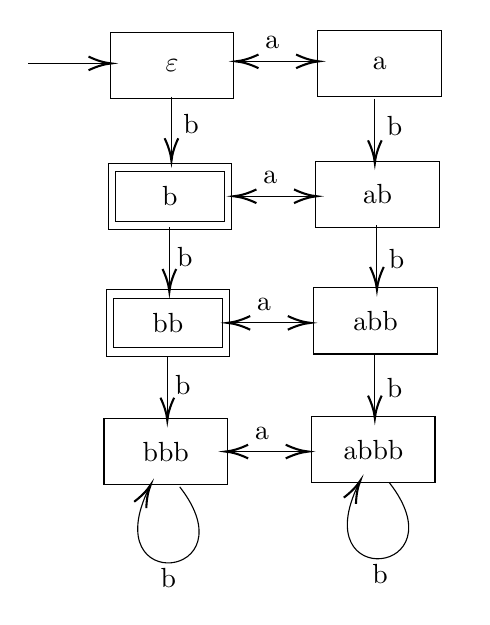
\begin{tikzpicture}[x=0.75pt,y=0.75pt,yscale=-1,xscale=1]
		%uncomment if require: \path (0,303.3999938964844); %set diagram left start at 0, and has height of 303.3999938964844
		
		%Shape: Rectangle [id:dp29401171660900416] 
		\draw   (252,16) -- (311.5,16) -- (311.5,47.91) -- (252,47.91) -- cycle ;
		%Straight Lines [id:da820770668159658] 
		\draw    (212.5,30.91) -- (250.5,30.91) ;
		\draw [shift={(252.5,30.91)}, rotate = 180] [color={rgb, 255:red, 0; green, 0; blue, 0 }  ][line width=0.75]    (10.93,-3.29) .. controls (6.95,-1.4) and (3.31,-0.3) .. (0,0) .. controls (3.31,0.3) and (6.95,1.4) .. (10.93,3.29)   ;
		
		%Straight Lines [id:da1659545540495566] 
		\draw    (281.5,46.91) -- (281.5,75.91) ;
		\draw [shift={(281.5,77.91)}, rotate = 270] [color={rgb, 255:red, 0; green, 0; blue, 0 }  ][line width=0.75]    (10.93,-3.29) .. controls (6.95,-1.4) and (3.31,-0.3) .. (0,0) .. controls (3.31,0.3) and (6.95,1.4) .. (10.93,3.29)   ;
		
		%Shape: Rectangle [id:dp9191047042549463] 
		\draw   (352,15) -- (411.5,15) -- (411.5,46.91) -- (352,46.91) -- cycle ;
		%Straight Lines [id:da12196753827571416] 
		\draw    (314.5,29.91) -- (350.5,29.91) ;
		\draw [shift={(352.5,29.91)}, rotate = 180] [color={rgb, 255:red, 0; green, 0; blue, 0 }  ][line width=0.75]    (10.93,-3.29) .. controls (6.95,-1.4) and (3.31,-0.3) .. (0,0) .. controls (3.31,0.3) and (6.95,1.4) .. (10.93,3.29)   ;
		\draw [shift={(312.5,29.91)}, rotate = 0] [color={rgb, 255:red, 0; green, 0; blue, 0 }  ][line width=0.75]    (10.93,-3.29) .. controls (6.95,-1.4) and (3.31,-0.3) .. (0,0) .. controls (3.31,0.3) and (6.95,1.4) .. (10.93,3.29)   ;
		%Shape: Rectangle [id:dp4319431310879662] 
		\draw   (251,79) -- (310.5,79) -- (310.5,110.91) -- (251,110.91) -- cycle ;
		%Straight Lines [id:da8851197451542516] 
		\draw    (280.5,109.91) -- (280.5,138.91) ;
		\draw [shift={(280.5,140.91)}, rotate = 270] [color={rgb, 255:red, 0; green, 0; blue, 0 }  ][line width=0.75]    (10.93,-3.29) .. controls (6.95,-1.4) and (3.31,-0.3) .. (0,0) .. controls (3.31,0.3) and (6.95,1.4) .. (10.93,3.29)   ;
		
		%Shape: Rectangle [id:dp1069532145737142] 
		\draw   (351,78) -- (410.5,78) -- (410.5,109.91) -- (351,109.91) -- cycle ;
		%Straight Lines [id:da5619068696089478] 
		\draw    (380.5,108.91) -- (380.5,137.91) ;
		\draw [shift={(380.5,139.91)}, rotate = 270] [color={rgb, 255:red, 0; green, 0; blue, 0 }  ][line width=0.75]    (10.93,-3.29) .. controls (6.95,-1.4) and (3.31,-0.3) .. (0,0) .. controls (3.31,0.3) and (6.95,1.4) .. (10.93,3.29)   ;
		
		%Shape: Rectangle [id:dp22578767988203263] 
		\draw   (250,140) -- (309.5,140) -- (309.5,171.91) -- (250,171.91) -- cycle ;
		%Shape: Rectangle [id:dp1954909148719357] 
		\draw   (350,139) -- (409.5,139) -- (409.5,170.91) -- (350,170.91) -- cycle ;
		%Straight Lines [id:da2606713471311273] 
		\draw    (313.5,94.91) -- (349.5,94.91) ;
		\draw [shift={(351.5,94.91)}, rotate = 180] [color={rgb, 255:red, 0; green, 0; blue, 0 }  ][line width=0.75]    (10.93,-3.29) .. controls (6.95,-1.4) and (3.31,-0.3) .. (0,0) .. controls (3.31,0.3) and (6.95,1.4) .. (10.93,3.29)   ;
		\draw [shift={(311.5,94.91)}, rotate = 0] [color={rgb, 255:red, 0; green, 0; blue, 0 }  ][line width=0.75]    (10.93,-3.29) .. controls (6.95,-1.4) and (3.31,-0.3) .. (0,0) .. controls (3.31,0.3) and (6.95,1.4) .. (10.93,3.29)   ;
		%Straight Lines [id:da4672369585241689] 
		\draw    (310.5,155.91) -- (346.5,155.91) ;
		\draw [shift={(348.5,155.91)}, rotate = 180] [color={rgb, 255:red, 0; green, 0; blue, 0 }  ][line width=0.75]    (10.93,-3.29) .. controls (6.95,-1.4) and (3.31,-0.3) .. (0,0) .. controls (3.31,0.3) and (6.95,1.4) .. (10.93,3.29)   ;
		\draw [shift={(308.5,155.91)}, rotate = 0] [color={rgb, 255:red, 0; green, 0; blue, 0 }  ][line width=0.75]    (10.93,-3.29) .. controls (6.95,-1.4) and (3.31,-0.3) .. (0,0) .. controls (3.31,0.3) and (6.95,1.4) .. (10.93,3.29)   ;
		%Straight Lines [id:da24231198752108374] 
		\draw    (379.5,47.91) -- (379.5,76.91) ;
		\draw [shift={(379.5,78.91)}, rotate = 270] [color={rgb, 255:red, 0; green, 0; blue, 0 }  ][line width=0.75]    (10.93,-3.29) .. controls (6.95,-1.4) and (3.31,-0.3) .. (0,0) .. controls (3.31,0.3) and (6.95,1.4) .. (10.93,3.29)   ;
		
		%Straight Lines [id:da3435055572035808] 
		\draw    (279.5,171.91) -- (279.5,200.91) ;
		\draw [shift={(279.5,202.91)}, rotate = 270] [color={rgb, 255:red, 0; green, 0; blue, 0 }  ][line width=0.75]    (10.93,-3.29) .. controls (6.95,-1.4) and (3.31,-0.3) .. (0,0) .. controls (3.31,0.3) and (6.95,1.4) .. (10.93,3.29)   ;
		
		%Straight Lines [id:da4162633397215143] 
		\draw    (379.5,170.91) -- (379.5,199.91) ;
		\draw [shift={(379.5,201.91)}, rotate = 270] [color={rgb, 255:red, 0; green, 0; blue, 0 }  ][line width=0.75]    (10.93,-3.29) .. controls (6.95,-1.4) and (3.31,-0.3) .. (0,0) .. controls (3.31,0.3) and (6.95,1.4) .. (10.93,3.29)   ;
		
		%Shape: Rectangle [id:dp10228158874269822] 
		\draw   (249,202) -- (308.5,202) -- (308.5,233.91) -- (249,233.91) -- cycle ;
		%Shape: Rectangle [id:dp08139555361678075] 
		\draw   (349,201) -- (408.5,201) -- (408.5,232.91) -- (349,232.91) -- cycle ;
		%Curve Lines [id:da05887687295762567] 
		\draw    (285.5,234.91) .. controls (320.15,279.46) and (245.03,287.74) .. (270.69,235.51) ;
		\draw [shift={(271.5,233.91)}, rotate = 477.41] [color={rgb, 255:red, 0; green, 0; blue, 0 }  ][line width=0.75]    (10.93,-3.29) .. controls (6.95,-1.4) and (3.31,-0.3) .. (0,0) .. controls (3.31,0.3) and (6.95,1.4) .. (10.93,3.29)   ;
		
		%Curve Lines [id:da3172648302217007] 
		\draw    (386.5,232.91) .. controls (421.15,277.46) and (346.03,285.74) .. (371.69,233.51) ;
		\draw [shift={(372.5,231.91)}, rotate = 477.41] [color={rgb, 255:red, 0; green, 0; blue, 0 }  ][line width=0.75]    (10.93,-3.29) .. controls (6.95,-1.4) and (3.31,-0.3) .. (0,0) .. controls (3.31,0.3) and (6.95,1.4) .. (10.93,3.29)   ;
		
		%Straight Lines [id:da12111511880996106] 
		\draw    (309.5,217.91) -- (345.5,217.91) ;
		\draw [shift={(347.5,217.91)}, rotate = 180] [color={rgb, 255:red, 0; green, 0; blue, 0 }  ][line width=0.75]    (10.93,-3.29) .. controls (6.95,-1.4) and (3.31,-0.3) .. (0,0) .. controls (3.31,0.3) and (6.95,1.4) .. (10.93,3.29)   ;
		\draw [shift={(307.5,217.91)}, rotate = 0] [color={rgb, 255:red, 0; green, 0; blue, 0 }  ][line width=0.75]    (10.93,-3.29) .. controls (6.95,-1.4) and (3.31,-0.3) .. (0,0) .. controls (3.31,0.3) and (6.95,1.4) .. (10.93,3.29)   ;
		%Shape: Rectangle [id:dp9368453442498375] 
		\draw   (254.5,83) -- (307,83) -- (307,106.91) -- (254.5,106.91) -- cycle ;
		%Shape: Rectangle [id:dp06172261059152562] 
		\draw   (253.5,144) -- (306,144) -- (306,167.91) -- (253.5,167.91) -- cycle ;
		
		% Text Node
		\draw (330,21) node  [align=left] {a};
		% Text Node
		\draw (329,86) node  [align=left] {a};
		% Text Node
		\draw (326,147) node  [align=left] {a};
		% Text Node
		\draw (291,60) node  [align=left] {b};
		% Text Node
		\draw (389,61) node  [align=left] {b};
		% Text Node
		\draw (288,124) node  [align=left] {b};
		% Text Node
		\draw (390,125) node  [align=left] {b};
		% Text Node
		\draw (381.75,30.95) node  [align=left] {a};
		% Text Node
		\draw (280.75,94.95) node  [align=left] {b};
		% Text Node
		\draw (279.75,155.95) node  [align=left] {bb};
		% Text Node
		\draw (380.75,93.95) node  [align=left] {ab};
		% Text Node
		\draw (379.75,154.95) node  [align=left] {abb};
		% Text Node
		\draw (325,209) node  [align=left] {a};
		% Text Node
		\draw (287,186) node  [align=left] {b};
		% Text Node
		\draw (389,187) node  [align=left] {b};
		% Text Node
		\draw (280,279) node  [align=left] {b};
		% Text Node
		\draw (382,277) node  [align=left] {b};
		% Text Node
		\draw (278.75,217.95) node  [align=left] {bbb};
		% Text Node
		\draw (378.75,216.95) node  [align=left] {abbb};
		% Text Node
		\draw (281.75,31.95) node  [align=left] {$\displaystyle \varepsilon $};
		
		\end{tikzpicture}

		\item[(e)]
		$L_1$ = $\{$w $|$ w starts with an a $\}$ = $\{ \: \{\varepsilon, a, b\}, \{a, b\}, \delta_a, \varepsilon, a\}$	\\
		$\delta_a = 
		\begin{array}{ c|c c }
			 & a & b\\
			\hline
			\varepsilon & a & b\\
			\hline
			a & a & a\\
			\hline
			b & b & b
		\end{array}$\\

		$L_2$ = $\{$w $|$ w has at most one b $\}$	= $\{ \: \{\varepsilon, b, bb\}, \{a, b\}, \delta_b, \varepsilon, \{\varepsilon, b\} \}$	\\
		$\delta_b = 
		\begin{array}{ c|c c }
			 & a & b\\
			\hline
			\varepsilon & \varepsilon & b\\
			\hline
			b & b & bb\\
			\hline
			bb & bb & bb
		\end{array}$\\

		Combining $L_1$ and $L_2$

		\tikzset{every picture/.style={line width=0.75pt}} %set default line width to 0.75pt        
		
		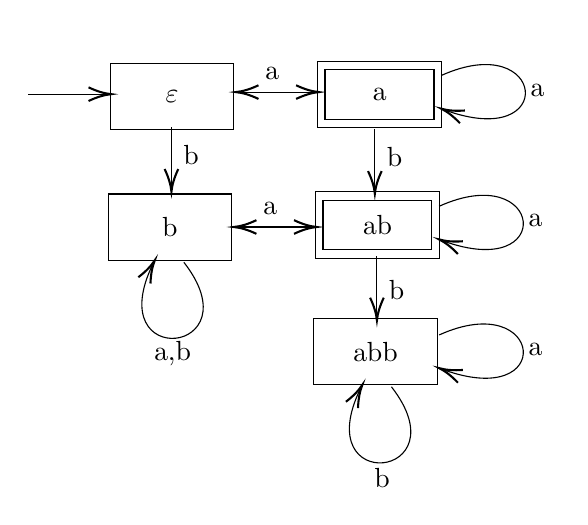
\begin{tikzpicture}[x=0.75pt,y=0.75pt,yscale=-1,xscale=1]
		%uncomment if require: \path (0,303.3999938964844); %set diagram left start at 0, and has height of 303.3999938964844
		
		%Shape: Rectangle [id:dp7446179682283836] 
		\draw   (252,16) -- (311.5,16) -- (311.5,47.91) -- (252,47.91) -- cycle ;
		%Straight Lines [id:da07346443767912447] 
		\draw    (212.5,30.91) -- (250.5,30.91) ;
		\draw [shift={(252.5,30.91)}, rotate = 180] [color={rgb, 255:red, 0; green, 0; blue, 0 }  ][line width=0.75]    (10.93,-3.29) .. controls (6.95,-1.4) and (3.31,-0.3) .. (0,0) .. controls (3.31,0.3) and (6.95,1.4) .. (10.93,3.29)   ;
		
		%Straight Lines [id:da4880112707021824] 
		\draw    (281.5,46.91) -- (281.5,75.91) ;
		\draw [shift={(281.5,77.91)}, rotate = 270] [color={rgb, 255:red, 0; green, 0; blue, 0 }  ][line width=0.75]    (10.93,-3.29) .. controls (6.95,-1.4) and (3.31,-0.3) .. (0,0) .. controls (3.31,0.3) and (6.95,1.4) .. (10.93,3.29)   ;
		
		%Shape: Rectangle [id:dp026346851428137752] 
		\draw   (352,15) -- (411.5,15) -- (411.5,46.91) -- (352,46.91) -- cycle ;
		%Straight Lines [id:da9251067147180454] 
		\draw    (314.5,29.91) -- (350.5,29.91) ;
		\draw [shift={(352.5,29.91)}, rotate = 180] [color={rgb, 255:red, 0; green, 0; blue, 0 }  ][line width=0.75]    (10.93,-3.29) .. controls (6.95,-1.4) and (3.31,-0.3) .. (0,0) .. controls (3.31,0.3) and (6.95,1.4) .. (10.93,3.29)   ;
		\draw [shift={(312.5,29.91)}, rotate = 0] [color={rgb, 255:red, 0; green, 0; blue, 0 }  ][line width=0.75]    (10.93,-3.29) .. controls (6.95,-1.4) and (3.31,-0.3) .. (0,0) .. controls (3.31,0.3) and (6.95,1.4) .. (10.93,3.29)   ;
		%Shape: Rectangle [id:dp7953987279658228] 
		\draw   (251,79) -- (310.5,79) -- (310.5,110.91) -- (251,110.91) -- cycle ;
		%Shape: Rectangle [id:dp15821492322429043] 
		\draw   (351,78) -- (410.5,78) -- (410.5,109.91) -- (351,109.91) -- cycle ;
		%Straight Lines [id:da5313743035830001] 
		\draw    (380.5,108.91) -- (380.5,137.91) ;
		\draw [shift={(380.5,139.91)}, rotate = 270] [color={rgb, 255:red, 0; green, 0; blue, 0 }  ][line width=0.75]    (10.93,-3.29) .. controls (6.95,-1.4) and (3.31,-0.3) .. (0,0) .. controls (3.31,0.3) and (6.95,1.4) .. (10.93,3.29)   ;
		
		%Shape: Rectangle [id:dp5914933594096616] 
		\draw   (350,139) -- (409.5,139) -- (409.5,170.91) -- (350,170.91) -- cycle ;
		%Straight Lines [id:da9371748617140896] 
		\draw    (313.5,94.91) -- (349.5,94.91) ;
		\draw [shift={(351.5,94.91)}, rotate = 180] [color={rgb, 255:red, 0; green, 0; blue, 0 }  ][line width=0.75]    (10.93,-3.29) .. controls (6.95,-1.4) and (3.31,-0.3) .. (0,0) .. controls (3.31,0.3) and (6.95,1.4) .. (10.93,3.29)   ;
		\draw [shift={(311.5,94.91)}, rotate = 0] [color={rgb, 255:red, 0; green, 0; blue, 0 }  ][line width=0.75]    (10.93,-3.29) .. controls (6.95,-1.4) and (3.31,-0.3) .. (0,0) .. controls (3.31,0.3) and (6.95,1.4) .. (10.93,3.29)   ;
		%Straight Lines [id:da3533313935558997] 
		\draw    (379.5,47.91) -- (379.5,76.91) ;
		\draw [shift={(379.5,78.91)}, rotate = 270] [color={rgb, 255:red, 0; green, 0; blue, 0 }  ][line width=0.75]    (10.93,-3.29) .. controls (6.95,-1.4) and (3.31,-0.3) .. (0,0) .. controls (3.31,0.3) and (6.95,1.4) .. (10.93,3.29)   ;
		
		%Curve Lines [id:da5234460237076906] 
		\draw    (287.5,111.91) .. controls (322.15,156.46) and (247.03,164.74) .. (272.69,112.51) ;
		\draw [shift={(273.5,110.91)}, rotate = 477.41] [color={rgb, 255:red, 0; green, 0; blue, 0 }  ][line width=0.75]    (10.93,-3.29) .. controls (6.95,-1.4) and (3.31,-0.3) .. (0,0) .. controls (3.31,0.3) and (6.95,1.4) .. (10.93,3.29)   ;
		
		%Curve Lines [id:da6306202840768786] 
		\draw    (387.5,171.91) .. controls (422.15,216.46) and (347.03,224.74) .. (372.69,172.51) ;
		\draw [shift={(373.5,170.91)}, rotate = 477.41] [color={rgb, 255:red, 0; green, 0; blue, 0 }  ][line width=0.75]    (10.93,-3.29) .. controls (6.95,-1.4) and (3.31,-0.3) .. (0,0) .. controls (3.31,0.3) and (6.95,1.4) .. (10.93,3.29)   ;
		
		%Shape: Rectangle [id:dp6325116269074724] 
		\draw   (354.5,82) -- (407,82) -- (407,105.91) -- (354.5,105.91) -- cycle ;
		%Shape: Rectangle [id:dp9773463769222948] 
		\draw   (355.5,19) -- (408,19) -- (408,42.91) -- (355.5,42.91) -- cycle ;
		%Curve Lines [id:da4888258610158267] 
		\draw    (411.5,21.91) .. controls (461.99,-0.86) and (468.38,58.69) .. (413.19,38.54) ;
		\draw [shift={(411.5,37.91)}, rotate = 381.1] [color={rgb, 255:red, 0; green, 0; blue, 0 }  ][line width=0.75]    (10.93,-3.29) .. controls (6.95,-1.4) and (3.31,-0.3) .. (0,0) .. controls (3.31,0.3) and (6.95,1.4) .. (10.93,3.29)   ;
		
		%Curve Lines [id:da6125946495310148] 
		\draw    (410.5,84.91) .. controls (460.99,62.14) and (467.38,121.69) .. (412.19,101.54) ;
		\draw [shift={(410.5,100.91)}, rotate = 381.1] [color={rgb, 255:red, 0; green, 0; blue, 0 }  ][line width=0.75]    (10.93,-3.29) .. controls (6.95,-1.4) and (3.31,-0.3) .. (0,0) .. controls (3.31,0.3) and (6.95,1.4) .. (10.93,3.29)   ;
		
		%Curve Lines [id:da4107204678195939] 
		\draw    (410.5,146.91) .. controls (460.99,124.14) and (467.38,183.69) .. (412.19,163.54) ;
		\draw [shift={(410.5,162.91)}, rotate = 381.1] [color={rgb, 255:red, 0; green, 0; blue, 0 }  ][line width=0.75]    (10.93,-3.29) .. controls (6.95,-1.4) and (3.31,-0.3) .. (0,0) .. controls (3.31,0.3) and (6.95,1.4) .. (10.93,3.29)   ;
		
		
		% Text Node
		\draw (330,21) node  [align=left] {a};
		% Text Node
		\draw (329,86) node  [align=left] {a};
		% Text Node
		\draw (291,60) node  [align=left] {b};
		% Text Node
		\draw (389,61) node  [align=left] {b};
		% Text Node
		\draw (390,125) node  [align=left] {b};
		% Text Node
		\draw (381.75,30.95) node  [align=left] {a};
		% Text Node
		\draw (280.75,94.95) node  [align=left] {b};
		% Text Node
		\draw (380.75,93.95) node  [align=left] {ab};
		% Text Node
		\draw (379.75,154.95) node  [align=left] {abb};
		% Text Node
		\draw (282,156) node  [align=left] {a,b};
		% Text Node
		\draw (383,216) node  [align=left] {b};
		% Text Node
		\draw (281.75,31.95) node  [align=left] {$\displaystyle \varepsilon $};
		% Text Node
		\draw (457.75,28.95) node  [align=left] {a};
		% Text Node
		\draw (456.75,91.95) node  [align=left] {a};
		% Text Node
		\draw (456.75,153.95) node  [align=left] {a};
		
		\end{tikzpicture}

		\item[(f)]
			$L_1$ = $\{$w $|$ w has odd number of a's $\}$ = $\{ \: \{\varepsilon, a\}, \{a, b\}, \delta_a, \varepsilon, a\}$	\\
		$\delta_a = 
			\begin{array}{ c|c c }
			 & a & b\\
			\hline
			\varepsilon & a & \varepsilon\\
			\hline
			a & \varepsilon & a
		\end{array}$\\

		$L_2$ = $\{$w $|$ w ends with b $\}$	= $\{ \: \{\varepsilon, b\}, \{a, b\}, \delta_b, \varepsilon, b \}$	\\
		$\delta_b = 
		\begin{array}{ c|c c }
			 & a & b\\
			\hline
			\varepsilon & \varepsilon & b\\
			\hline
			b & \varepsilon & b
		\end{array}$\\

		Combining $L_1$ and $L_2$

		\tikzset{every picture/.style={line width=0.75pt}} %set default line width to 0.75pt        
		
		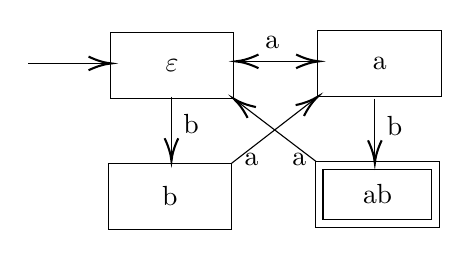
\begin{tikzpicture}[x=0.75pt,y=0.75pt,yscale=-1,xscale=1]
		%uncomment if require: \path (0,573.90625); %set diagram left start at 0, and has height of 573.90625
		
		%Shape: Rectangle [id:dp7378347097751705] 
		\draw   (169,305) -- (228.5,305) -- (228.5,336.91) -- (169,336.91) -- cycle ;
		%Straight Lines [id:da9181037703414214] 
		\draw    (129.5,319.91) -- (167.5,319.91) ;
		\draw [shift={(169.5,319.91)}, rotate = 180] [color={rgb, 255:red, 0; green, 0; blue, 0 }  ][line width=0.75]    (10.93,-3.29) .. controls (6.95,-1.4) and (3.31,-0.3) .. (0,0) .. controls (3.31,0.3) and (6.95,1.4) .. (10.93,3.29)   ;
		
		%Straight Lines [id:da12026730605356528] 
		\draw    (198.5,335.91) -- (198.5,364.91) ;
		\draw [shift={(198.5,366.91)}, rotate = 270] [color={rgb, 255:red, 0; green, 0; blue, 0 }  ][line width=0.75]    (10.93,-3.29) .. controls (6.95,-1.4) and (3.31,-0.3) .. (0,0) .. controls (3.31,0.3) and (6.95,1.4) .. (10.93,3.29)   ;
		
		%Shape: Rectangle [id:dp7397295574767186] 
		\draw   (269,304) -- (328.5,304) -- (328.5,335.91) -- (269,335.91) -- cycle ;
		%Straight Lines [id:da6041386820089447] 
		\draw    (231.5,318.91) -- (267.5,318.91) ;
		\draw [shift={(269.5,318.91)}, rotate = 180] [color={rgb, 255:red, 0; green, 0; blue, 0 }  ][line width=0.75]    (10.93,-3.29) .. controls (6.95,-1.4) and (3.31,-0.3) .. (0,0) .. controls (3.31,0.3) and (6.95,1.4) .. (10.93,3.29)   ;
		\draw [shift={(229.5,318.91)}, rotate = 0] [color={rgb, 255:red, 0; green, 0; blue, 0 }  ][line width=0.75]    (10.93,-3.29) .. controls (6.95,-1.4) and (3.31,-0.3) .. (0,0) .. controls (3.31,0.3) and (6.95,1.4) .. (10.93,3.29)   ;
		%Shape: Rectangle [id:dp0677374903382102] 
		\draw   (168,368) -- (227.5,368) -- (227.5,399.91) -- (168,399.91) -- cycle ;
		%Shape: Rectangle [id:dp1701553615000866] 
		\draw   (268,367) -- (327.5,367) -- (327.5,398.91) -- (268,398.91) -- cycle ;
		%Straight Lines [id:da9895033325742377] 
		\draw    (296.5,336.91) -- (296.5,365.91) ;
		\draw [shift={(296.5,367.91)}, rotate = 270] [color={rgb, 255:red, 0; green, 0; blue, 0 }  ][line width=0.75]    (10.93,-3.29) .. controls (6.95,-1.4) and (3.31,-0.3) .. (0,0) .. controls (3.31,0.3) and (6.95,1.4) .. (10.93,3.29)   ;
		
		%Straight Lines [id:da2523770362732587] 
		\draw    (230.09,338.12) -- (268,367) ;
		
		\draw [shift={(228.5,336.91)}, rotate = 37.3] [color={rgb, 255:red, 0; green, 0; blue, 0 }  ][line width=0.75]    (10.93,-3.29) .. controls (6.95,-1.4) and (3.31,-0.3) .. (0,0) .. controls (3.31,0.3) and (6.95,1.4) .. (10.93,3.29)   ;
		%Straight Lines [id:da3075017339957038] 
		\draw    (227.5,368) -- (267.42,337.13) ;
		\draw [shift={(269,335.91)}, rotate = 502.28] [color={rgb, 255:red, 0; green, 0; blue, 0 }  ][line width=0.75]    (10.93,-3.29) .. controls (6.95,-1.4) and (3.31,-0.3) .. (0,0) .. controls (3.31,0.3) and (6.95,1.4) .. (10.93,3.29)   ;
		
		%Shape: Rectangle [id:dp9510770723795476] 
		\draw   (271.5,371) -- (324,371) -- (324,394.91) -- (271.5,394.91) -- cycle ;
		
		% Text Node
		\draw (247,310) node  [align=left] {a};
		% Text Node
		\draw (208,349) node  [align=left] {b};
		% Text Node
		\draw (306,350) node  [align=left] {b};
		% Text Node
		\draw (198.75,320.95) node  [align=left] {$\varepsilon$};
		% Text Node
		\draw (298.75,319.95) node  [align=left] {a};
		% Text Node
		\draw (197.75,383.95) node  [align=left] {b};
		% Text Node
		\draw (297.75,382.95) node  [align=left] {ab};
		% Text Node
		\draw (260,366) node  [align=left] {a};
		% Text Node
		\draw (237,366) node  [align=left] {a};
		
		\end{tikzpicture}

		\item[(g)]
			$L_1$ = $\{$w $|$ w has even length $\}$ = $\{ \: \{\varepsilon, a, b, ab\}, \{a, b\}, \delta_a, \varepsilon, \{\varepsilon, ab\}\}$	\\
		$\delta_a = 
		\begin{array}{ c|c c }
			 & a & b\\
			\hline
			\varepsilon & a & b\\
			\hline
			a & \varepsilon & ab\\
			\hline
			b & ab & \varepsilon\\
			\hline
			ab & b & a
		\end{array}$\\

		$L_2$ = $\{$w $|$ w has odd number of a's $\}$	= $\{ \: \{\varepsilon, a\}, \{a, b\}, \delta_b, \varepsilon, a \}$	\\
		$\delta_b = 
			\begin{array}{ c|c c }
			 & a & b\\
			\hline
			\varepsilon & a & \varepsilon\\
			\hline
			a & \varepsilon & a
		\end{array}$\\

		Combining $L_1$ and $L_2$
		\tikzset{every picture/.style={line width=0.75pt}} %set default line width to 0.75pt        
		
		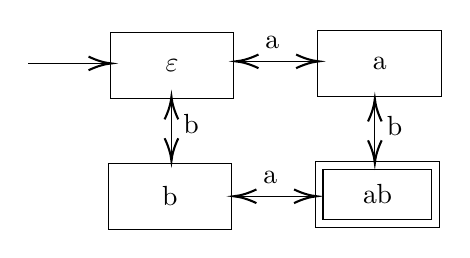
\begin{tikzpicture}[x=0.75pt,y=0.75pt,yscale=-1,xscale=1]
		%uncomment if require: \path (0,573.90625); %set diagram left start at 0, and has height of 573.90625
		
		%Shape: Rectangle [id:dp7378347097751705] 
		\draw   (169,305) -- (228.5,305) -- (228.5,336.91) -- (169,336.91) -- cycle ;
		%Straight Lines [id:da9181037703414214] 
		\draw    (129.5,319.91) -- (167.5,319.91) ;
		\draw [shift={(169.5,319.91)}, rotate = 180] [color={rgb, 255:red, 0; green, 0; blue, 0 }  ][line width=0.75]    (10.93,-3.29) .. controls (6.95,-1.4) and (3.31,-0.3) .. (0,0) .. controls (3.31,0.3) and (6.95,1.4) .. (10.93,3.29)   ;
		
		%Straight Lines [id:da12026730605356528] 
		\draw    (198.5,337.91) -- (198.5,364.91) ;
		\draw [shift={(198.5,366.91)}, rotate = 270] [color={rgb, 255:red, 0; green, 0; blue, 0 }  ][line width=0.75]    (10.93,-3.29) .. controls (6.95,-1.4) and (3.31,-0.3) .. (0,0) .. controls (3.31,0.3) and (6.95,1.4) .. (10.93,3.29)   ;
		\draw [shift={(198.5,335.91)}, rotate = 90] [color={rgb, 255:red, 0; green, 0; blue, 0 }  ][line width=0.75]    (10.93,-3.29) .. controls (6.95,-1.4) and (3.31,-0.3) .. (0,0) .. controls (3.31,0.3) and (6.95,1.4) .. (10.93,3.29)   ;
		%Shape: Rectangle [id:dp7397295574767186] 
		\draw   (269,304) -- (328.5,304) -- (328.5,335.91) -- (269,335.91) -- cycle ;
		%Straight Lines [id:da6041386820089447] 
		\draw    (231.5,318.91) -- (267.5,318.91) ;
		\draw [shift={(269.5,318.91)}, rotate = 180] [color={rgb, 255:red, 0; green, 0; blue, 0 }  ][line width=0.75]    (10.93,-3.29) .. controls (6.95,-1.4) and (3.31,-0.3) .. (0,0) .. controls (3.31,0.3) and (6.95,1.4) .. (10.93,3.29)   ;
		\draw [shift={(229.5,318.91)}, rotate = 0] [color={rgb, 255:red, 0; green, 0; blue, 0 }  ][line width=0.75]    (10.93,-3.29) .. controls (6.95,-1.4) and (3.31,-0.3) .. (0,0) .. controls (3.31,0.3) and (6.95,1.4) .. (10.93,3.29)   ;
		%Shape: Rectangle [id:dp0677374903382102] 
		\draw   (168,368) -- (227.5,368) -- (227.5,399.91) -- (168,399.91) -- cycle ;
		%Shape: Rectangle [id:dp1701553615000866] 
		\draw   (268,367) -- (327.5,367) -- (327.5,398.91) -- (268,398.91) -- cycle ;
		%Straight Lines [id:da2676897637415887] 
		\draw    (230.5,383.91) -- (266.5,383.91) ;
		\draw [shift={(268.5,383.91)}, rotate = 180] [color={rgb, 255:red, 0; green, 0; blue, 0 }  ][line width=0.75]    (10.93,-3.29) .. controls (6.95,-1.4) and (3.31,-0.3) .. (0,0) .. controls (3.31,0.3) and (6.95,1.4) .. (10.93,3.29)   ;
		\draw [shift={(228.5,383.91)}, rotate = 0] [color={rgb, 255:red, 0; green, 0; blue, 0 }  ][line width=0.75]    (10.93,-3.29) .. controls (6.95,-1.4) and (3.31,-0.3) .. (0,0) .. controls (3.31,0.3) and (6.95,1.4) .. (10.93,3.29)   ;
		%Straight Lines [id:da9895033325742377] 
		\draw    (296.5,338.91) -- (296.5,365.91) ;
		\draw [shift={(296.5,367.91)}, rotate = 270] [color={rgb, 255:red, 0; green, 0; blue, 0 }  ][line width=0.75]    (10.93,-3.29) .. controls (6.95,-1.4) and (3.31,-0.3) .. (0,0) .. controls (3.31,0.3) and (6.95,1.4) .. (10.93,3.29)   ;
		\draw [shift={(296.5,336.91)}, rotate = 90] [color={rgb, 255:red, 0; green, 0; blue, 0 }  ][line width=0.75]    (10.93,-3.29) .. controls (6.95,-1.4) and (3.31,-0.3) .. (0,0) .. controls (3.31,0.3) and (6.95,1.4) .. (10.93,3.29)   ;
		%Shape: Rectangle [id:dp30975186962948253] 
		\draw   (271.5,371) -- (324,371) -- (324,394.91) -- (271.5,394.91) -- cycle ;
		
		% Text Node
		\draw (247,310) node  [align=left] {a};
		% Text Node
		\draw (246,375) node  [align=left] {a};
		% Text Node
		\draw (208,349) node  [align=left] {b};
		% Text Node
		\draw (306,350) node  [align=left] {b};
		% Text Node
		\draw (198.75,320.95) node  [align=left] {$\varepsilon$};
		% Text Node
		\draw (298.75,319.95) node  [align=left] {a};
		% Text Node
		\draw (197.75,383.95) node  [align=left] {b};
		% Text Node
		\draw (297.75,382.95) node  [align=left] {ab};
		
		\end{tikzpicture}

\end{enumerate}

\begin{problem}{1.5}
\end{problem}
\begin{enumerate}
	\item[(c)]
		L = $\{ \:\{\varepsilon, a, b, ab, ba\}, \{a, b\}, \delta, \varepsilon, \{a, b\}\}$	\\
		$\delta = 
		\begin{array}{ c|c|c }
			 & a & b\\
			\hline
			\varepsilon & a & b\\
			\hline
			a & a & ab\\
			\hline
			b & b & ba\\
			\hline
			ab & ab & ab\\
			\hline
			ba & ba & ba
		\end{array}$\\
		
		State diagram:

		\tikzset{every picture/.style={line width=0.75pt}} %set default line width to 0.75pt        
		
		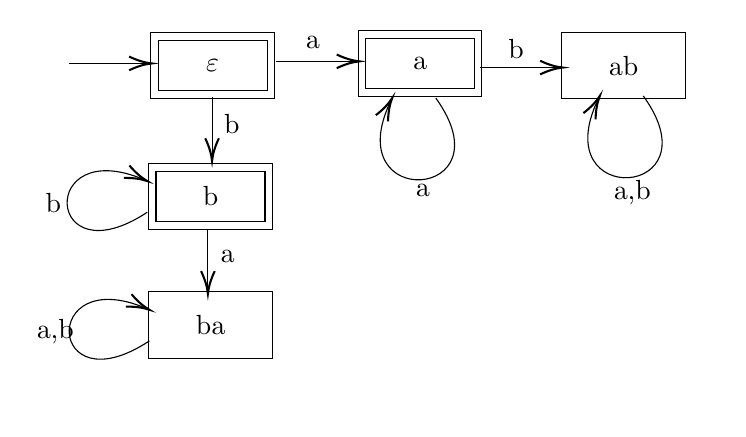
\begin{tikzpicture}[x=0.75pt,y=0.75pt,yscale=-1,xscale=1]
		%uncomment if require: \path (0,188.60000610351562); %set diagram left start at 0, and has height of 188.60000610351562
		
		%Shape: Rectangle [id:dp14834589965525913] 
		\draw   (225,17) -- (284.5,17) -- (284.5,48.91) -- (225,48.91) -- cycle ;
		%Straight Lines [id:da4250561285702925] 
		\draw    (185.5,31.91) -- (223.5,31.91) ;
		\draw [shift={(225.5,31.91)}, rotate = 180] [color={rgb, 255:red, 0; green, 0; blue, 0 }  ][line width=0.75]    (10.93,-3.29) .. controls (6.95,-1.4) and (3.31,-0.3) .. (0,0) .. controls (3.31,0.3) and (6.95,1.4) .. (10.93,3.29)   ;
		
		%Straight Lines [id:da5734070371316622] 
		\draw    (254.5,47.91) -- (254.5,76.91) ;
		\draw [shift={(254.5,78.91)}, rotate = 270] [color={rgb, 255:red, 0; green, 0; blue, 0 }  ][line width=0.75]    (10.93,-3.29) .. controls (6.95,-1.4) and (3.31,-0.3) .. (0,0) .. controls (3.31,0.3) and (6.95,1.4) .. (10.93,3.29)   ;
		
		%Shape: Rectangle [id:dp8955761321680229] 
		\draw   (325,16) -- (384.5,16) -- (384.5,47.91) -- (325,47.91) -- cycle ;
		%Straight Lines [id:da3409234438009763] 
		\draw    (285.5,30.91) -- (323.5,30.91) ;
		\draw [shift={(325.5,30.91)}, rotate = 180] [color={rgb, 255:red, 0; green, 0; blue, 0 }  ][line width=0.75]    (10.93,-3.29) .. controls (6.95,-1.4) and (3.31,-0.3) .. (0,0) .. controls (3.31,0.3) and (6.95,1.4) .. (10.93,3.29)   ;
		
		%Shape: Rectangle [id:dp1288469522241673] 
		\draw   (224,80) -- (283.5,80) -- (283.5,111.91) -- (224,111.91) -- cycle ;
		%Shape: Rectangle [id:dp14520173544268378] 
		\draw   (224,142) -- (283.5,142) -- (283.5,173.91) -- (224,173.91) -- cycle ;
		%Straight Lines [id:da5916523231625537] 
		\draw    (252.5,111.91) -- (252.5,140.91) ;
		\draw [shift={(252.5,142.91)}, rotate = 270] [color={rgb, 255:red, 0; green, 0; blue, 0 }  ][line width=0.75]    (10.93,-3.29) .. controls (6.95,-1.4) and (3.31,-0.3) .. (0,0) .. controls (3.31,0.3) and (6.95,1.4) .. (10.93,3.29)   ;
		
		%Shape: Rectangle [id:dp46275223178117164] 
		\draw   (423,17) -- (482.5,17) -- (482.5,48.91) -- (423,48.91) -- cycle ;
		%Straight Lines [id:da5536929252307312] 
		\draw    (383.5,33.91) -- (421.5,33.91) ;
		\draw [shift={(423.5,33.91)}, rotate = 180] [color={rgb, 255:red, 0; green, 0; blue, 0 }  ][line width=0.75]    (10.93,-3.29) .. controls (6.95,-1.4) and (3.31,-0.3) .. (0,0) .. controls (3.31,0.3) and (6.95,1.4) .. (10.93,3.29)   ;
		
		%Shape: Rectangle [id:dp364629817969951] 
		\draw   (227.5,84) -- (280,84) -- (280,107.91) -- (227.5,107.91) -- cycle ;
		%Shape: Rectangle [id:dp7731241942297908] 
		\draw   (328.5,20) -- (381,20) -- (381,43.91) -- (328.5,43.91) -- cycle ;
		%Curve Lines [id:da009647417876258224] 
		\draw    (223.3,103.6) .. controls (173.8,136.27) and (170.36,66.03) .. (221.73,87.91) ;
		\draw [shift={(223.3,88.6)}, rotate = 204.36] [color={rgb, 255:red, 0; green, 0; blue, 0 }  ][line width=0.75]    (10.93,-3.29) .. controls (6.95,-1.4) and (3.31,-0.3) .. (0,0) .. controls (3.31,0.3) and (6.95,1.4) .. (10.93,3.29)   ;
		
		%Curve Lines [id:da04327625125017276] 
		\draw    (362.3,48.6) .. controls (397.94,98.1) and (314.99,103.5) .. (340.49,50.23) ;
		\draw [shift={(341.3,48.6)}, rotate = 476.98] [color={rgb, 255:red, 0; green, 0; blue, 0 }  ][line width=0.75]    (10.93,-3.29) .. controls (6.95,-1.4) and (3.31,-0.3) .. (0,0) .. controls (3.31,0.3) and (6.95,1.4) .. (10.93,3.29)   ;
		
		%Curve Lines [id:da9143965887453047] 
		\draw    (462.3,47.6) .. controls (497.94,97.1) and (414.99,102.5) .. (440.49,49.23) ;
		\draw [shift={(441.3,47.6)}, rotate = 476.98] [color={rgb, 255:red, 0; green, 0; blue, 0 }  ][line width=0.75]    (10.93,-3.29) .. controls (6.95,-1.4) and (3.31,-0.3) .. (0,0) .. controls (3.31,0.3) and (6.95,1.4) .. (10.93,3.29)   ;
		
		%Curve Lines [id:da05156417596762619] 
		\draw    (224.3,165.6) .. controls (174.8,198.27) and (171.36,128.03) .. (222.73,149.91) ;
		\draw [shift={(224.3,150.6)}, rotate = 204.36] [color={rgb, 255:red, 0; green, 0; blue, 0 }  ][line width=0.75]    (10.93,-3.29) .. controls (6.95,-1.4) and (3.31,-0.3) .. (0,0) .. controls (3.31,0.3) and (6.95,1.4) .. (10.93,3.29)   ;
		
		%Shape: Rectangle [id:dp08047742120175094] 
		\draw   (228.5,21) -- (281,21) -- (281,44.91) -- (228.5,44.91) -- cycle ;
		
		% Text Node
		\draw (303,22) node  [align=left] {a};
		% Text Node
		\draw (264,61) node  [align=left] {b};
		% Text Node
		\draw (254.75,32.95) node  [align=left] {$\varepsilon$};
		% Text Node
		\draw (354.75,31.95) node  [align=left] {a};
		% Text Node
		\draw (253.75,95.95) node  [align=left] {b};
		% Text Node
		\draw (262,125) node  [align=left] {a};
		% Text Node
		\draw (253.75,157.95) node  [align=left] {ba};
		% Text Node
		\draw (401,25) node  [align=left] {b};
		% Text Node
		\draw (452.75,32.95) node  [align=left] {ab};
		% Text Node
		\draw (356,93) node  [align=left] {a};
		% Text Node
		\draw (178,99) node  [align=left] {b};
		% Text Node
		\draw (457,94) node  [align=left] {a,b};
		% Text Node
		\draw (179,161) node  [align=left] {a,b};
		
		\end{tikzpicture}

	\item[(d)]
		L = $\{ \:\{\varepsilon, a, b, ab, aba\}, \{a, b\}, \delta, \varepsilon, \{\varepsilon, a, b, aba\}\}$	\\
		$\delta = 
		\begin{array}{ c|c|c }
			 & a & b\\
			\hline
			\varepsilon  & a & b\\
			\hline
			a & a & ab\\
			\hline
			b & b & b\\
			\hline
			ab & aba & ab\\
			\hline
			aba & aba & aba
		\end{array}$\\
		
		State diagram:

		\tikzset{every picture/.style={line width=0.75pt}} %set default line width to 0.75pt        
		
		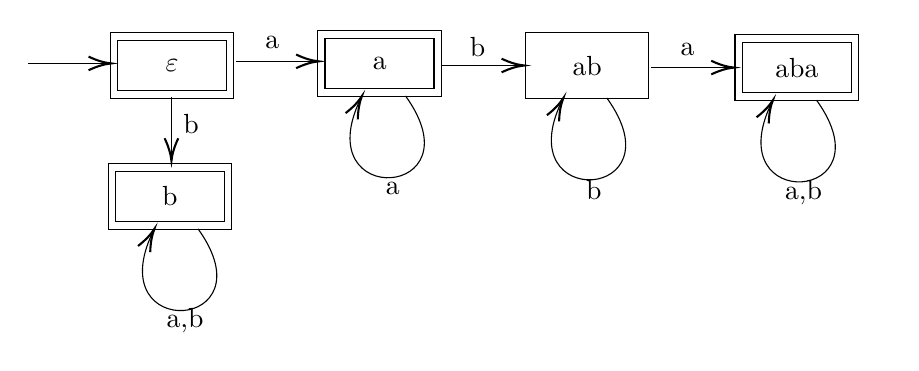
\begin{tikzpicture}[x=0.75pt,y=0.75pt,yscale=-1,xscale=1]
		%uncomment if require: \path (0,273.1999988555908); %set diagram left start at 0, and has height of 273.1999988555908
		
		%Shape: Rectangle [id:dp18934423767084785] 
		\draw   (238,51) -- (297.5,51) -- (297.5,82.91) -- (238,82.91) -- cycle ;
		%Straight Lines [id:da6758202938507798] 
		\draw    (198.5,65.91) -- (236.5,65.91) ;
		\draw [shift={(238.5,65.91)}, rotate = 180] [color={rgb, 255:red, 0; green, 0; blue, 0 }  ][line width=0.75]    (10.93,-3.29) .. controls (6.95,-1.4) and (3.31,-0.3) .. (0,0) .. controls (3.31,0.3) and (6.95,1.4) .. (10.93,3.29)   ;
		
		%Straight Lines [id:da060783689200354374] 
		\draw    (267.5,81.91) -- (267.5,110.91) ;
		\draw [shift={(267.5,112.91)}, rotate = 270] [color={rgb, 255:red, 0; green, 0; blue, 0 }  ][line width=0.75]    (10.93,-3.29) .. controls (6.95,-1.4) and (3.31,-0.3) .. (0,0) .. controls (3.31,0.3) and (6.95,1.4) .. (10.93,3.29)   ;
		
		%Shape: Rectangle [id:dp05838867870372222] 
		\draw   (338,50) -- (397.5,50) -- (397.5,81.91) -- (338,81.91) -- cycle ;
		%Straight Lines [id:da8747372471621973] 
		\draw    (298.5,64.91) -- (336.5,64.91) ;
		\draw [shift={(338.5,64.91)}, rotate = 180] [color={rgb, 255:red, 0; green, 0; blue, 0 }  ][line width=0.75]    (10.93,-3.29) .. controls (6.95,-1.4) and (3.31,-0.3) .. (0,0) .. controls (3.31,0.3) and (6.95,1.4) .. (10.93,3.29)   ;
		
		%Shape: Rectangle [id:dp605849658147853] 
		\draw   (237,114) -- (296.5,114) -- (296.5,145.91) -- (237,145.91) -- cycle ;
		%Shape: Rectangle [id:dp15115182476003364] 
		\draw   (438,51) -- (497.5,51) -- (497.5,82.91) -- (438,82.91) -- cycle ;
		%Straight Lines [id:da7507401117547379] 
		\draw    (397.5,66.91) -- (435.5,66.91) ;
		\draw [shift={(437.5,66.91)}, rotate = 180] [color={rgb, 255:red, 0; green, 0; blue, 0 }  ][line width=0.75]    (10.93,-3.29) .. controls (6.95,-1.4) and (3.31,-0.3) .. (0,0) .. controls (3.31,0.3) and (6.95,1.4) .. (10.93,3.29)   ;
		
		%Curve Lines [id:da5546339788003884] 
		\draw    (380.3,81.6) .. controls (415.94,131.1) and (332.99,136.5) .. (358.49,83.23) ;
		\draw [shift={(359.3,81.6)}, rotate = 476.98] [color={rgb, 255:red, 0; green, 0; blue, 0 }  ][line width=0.75]    (10.93,-3.29) .. controls (6.95,-1.4) and (3.31,-0.3) .. (0,0) .. controls (3.31,0.3) and (6.95,1.4) .. (10.93,3.29)   ;
		
		%Curve Lines [id:da8660642013995004] 
		\draw    (477.3,82.6) .. controls (512.94,132.1) and (429.99,137.5) .. (455.49,84.23) ;
		\draw [shift={(456.3,82.6)}, rotate = 476.98] [color={rgb, 255:red, 0; green, 0; blue, 0 }  ][line width=0.75]    (10.93,-3.29) .. controls (6.95,-1.4) and (3.31,-0.3) .. (0,0) .. controls (3.31,0.3) and (6.95,1.4) .. (10.93,3.29)   ;
		
		%Curve Lines [id:da5970080827269733] 
		\draw    (280.3,145.6) .. controls (315.94,195.1) and (232.99,200.5) .. (258.49,147.23) ;
		\draw [shift={(259.3,145.6)}, rotate = 476.98] [color={rgb, 255:red, 0; green, 0; blue, 0 }  ][line width=0.75]    (10.93,-3.29) .. controls (6.95,-1.4) and (3.31,-0.3) .. (0,0) .. controls (3.31,0.3) and (6.95,1.4) .. (10.93,3.29)   ;
		
		%Shape: Rectangle [id:dp663343191322924] 
		\draw   (240.5,118) -- (293,118) -- (293,141.91) -- (240.5,141.91) -- cycle ;
		%Shape: Rectangle [id:dp07647313265628153] 
		\draw   (341.5,54) -- (394,54) -- (394,77.91) -- (341.5,77.91) -- cycle ;
		%Shape: Rectangle [id:dp05575975111925513] 
		\draw   (241.5,55) -- (294,55) -- (294,78.91) -- (241.5,78.91) -- cycle ;
		%Shape: Rectangle [id:dp6235578871003251] 
		\draw   (539,52) -- (598.5,52) -- (598.5,83.91) -- (539,83.91) -- cycle ;
		%Straight Lines [id:da10508688328578941] 
		\draw    (498.5,67.91) -- (536.5,67.91) ;
		\draw [shift={(538.5,67.91)}, rotate = 180] [color={rgb, 255:red, 0; green, 0; blue, 0 }  ][line width=0.75]    (10.93,-3.29) .. controls (6.95,-1.4) and (3.31,-0.3) .. (0,0) .. controls (3.31,0.3) and (6.95,1.4) .. (10.93,3.29)   ;
		
		%Curve Lines [id:da004117431253814807] 
		\draw    (578.3,83.6) .. controls (613.94,133.1) and (530.99,138.5) .. (556.49,85.23) ;
		\draw [shift={(557.3,83.6)}, rotate = 476.98] [color={rgb, 255:red, 0; green, 0; blue, 0 }  ][line width=0.75]    (10.93,-3.29) .. controls (6.95,-1.4) and (3.31,-0.3) .. (0,0) .. controls (3.31,0.3) and (6.95,1.4) .. (10.93,3.29)   ;
		
		%Shape: Rectangle [id:dp7076450195046924] 
		\draw   (542.5,56) -- (595,56) -- (595,79.91) -- (542.5,79.91) -- cycle ;
		
		% Text Node
		\draw (316,56) node  [align=left] {a};
		% Text Node
		\draw (415,58) node  [align=left] {b};
		% Text Node
		\draw (277,95) node  [align=left] {b};
		% Text Node
		\draw (267.75,66.95) node  [align=left] {$\displaystyle \varepsilon $};
		% Text Node
		\draw (367.75,65.95) node  [align=left] {a};
		% Text Node
		\draw (467.75,66.95) node  [align=left] {ab};
		% Text Node
		\draw (266.75,129.95) node  [align=left] {b};
		% Text Node
		\draw (374,126) node  [align=left] {a};
		% Text Node
		\draw (471,127) node  [align=left] {b};
		% Text Node
		\draw (274,190) node  [align=left] {a,b};
		% Text Node
		\draw (516,59) node  [align=left] {a};
		% Text Node
		\draw (568.75,67.95) node  [align=left] {aba};
		% Text Node
		\draw (572,128) node  [align=left] {a,b};
		
		\end{tikzpicture}

	\item[(e)]
		L = $\{ \:\{\varepsilon, a, b, ab\}, \{a, b\}, \delta, \varepsilon, \{a, b\}\}$	\\
		$\delta = 
		\begin{array}{ c|c|c }
			 & a & b\\
			\hline
			\varepsilon  & a & b\\
			\hline
			a & b & ab\\
			\hline
			b & b & b\\
			\hline
			ab & a & ab
		\end{array}$\\
		
		State diagram:

		\tikzset{every picture/.style={line width=0.75pt}} %set default line width to 0.75pt        
		
		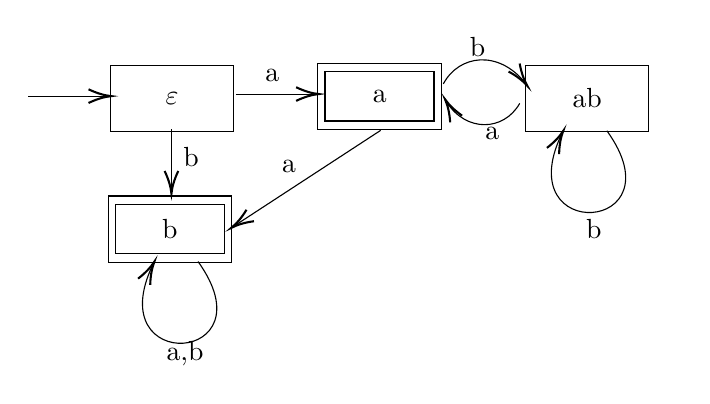
\begin{tikzpicture}[x=0.75pt,y=0.75pt,yscale=-1,xscale=1]
		%uncomment if require: \path (0,273.1999988555908); %set diagram left start at 0, and has height of 273.1999988555908
		
		%Shape: Rectangle [id:dp9160061878739032] 
		\draw   (238,51) -- (297.5,51) -- (297.5,82.91) -- (238,82.91) -- cycle ;
		%Straight Lines [id:da34580539091949336] 
		\draw    (198.5,65.91) -- (236.5,65.91) ;
		\draw [shift={(238.5,65.91)}, rotate = 180] [color={rgb, 255:red, 0; green, 0; blue, 0 }  ][line width=0.75]    (10.93,-3.29) .. controls (6.95,-1.4) and (3.31,-0.3) .. (0,0) .. controls (3.31,0.3) and (6.95,1.4) .. (10.93,3.29)   ;
		
		%Straight Lines [id:da5387802399128179] 
		\draw    (267.5,81.91) -- (267.5,110.91) ;
		\draw [shift={(267.5,112.91)}, rotate = 270] [color={rgb, 255:red, 0; green, 0; blue, 0 }  ][line width=0.75]    (10.93,-3.29) .. controls (6.95,-1.4) and (3.31,-0.3) .. (0,0) .. controls (3.31,0.3) and (6.95,1.4) .. (10.93,3.29)   ;
		
		%Shape: Rectangle [id:dp7034680123854398] 
		\draw   (338,50) -- (397.5,50) -- (397.5,81.91) -- (338,81.91) -- cycle ;
		%Straight Lines [id:da42944876106729724] 
		\draw    (298.5,64.91) -- (336.5,64.91) ;
		\draw [shift={(338.5,64.91)}, rotate = 180] [color={rgb, 255:red, 0; green, 0; blue, 0 }  ][line width=0.75]    (10.93,-3.29) .. controls (6.95,-1.4) and (3.31,-0.3) .. (0,0) .. controls (3.31,0.3) and (6.95,1.4) .. (10.93,3.29)   ;
		
		%Shape: Rectangle [id:dp7877421455035902] 
		\draw   (237,114) -- (296.5,114) -- (296.5,145.91) -- (237,145.91) -- cycle ;
		%Shape: Rectangle [id:dp5822822085047148] 
		\draw   (438,51) -- (497.5,51) -- (497.5,82.91) -- (438,82.91) -- cycle ;
		%Curve Lines [id:da4949267020847379] 
		\draw    (280.3,145.6) .. controls (315.94,195.1) and (232.99,200.5) .. (258.49,147.23) ;
		\draw [shift={(259.3,145.6)}, rotate = 476.98] [color={rgb, 255:red, 0; green, 0; blue, 0 }  ][line width=0.75]    (10.93,-3.29) .. controls (6.95,-1.4) and (3.31,-0.3) .. (0,0) .. controls (3.31,0.3) and (6.95,1.4) .. (10.93,3.29)   ;
		
		%Curve Lines [id:da5392919070194218] 
		\draw    (398.5,60) .. controls (406.07,45.84) and (425.11,43.53) .. (437.84,59.47) ;
		\draw [shift={(439,61)}, rotate = 234.19] [color={rgb, 255:red, 0; green, 0; blue, 0 }  ][line width=0.75]    (10.93,-3.29) .. controls (6.95,-1.4) and (3.31,-0.3) .. (0,0) .. controls (3.31,0.3) and (6.95,1.4) .. (10.93,3.29)   ;
		
		%Curve Lines [id:da44667745225759736] 
		\draw    (435.3,69.4) .. controls (427.58,82.91) and (409.62,83.38) .. (400.28,69.02) ;
		\draw [shift={(399.3,67.4)}, rotate = 420.64] [color={rgb, 255:red, 0; green, 0; blue, 0 }  ][line width=0.75]    (10.93,-3.29) .. controls (6.95,-1.4) and (3.31,-0.3) .. (0,0) .. controls (3.31,0.3) and (6.95,1.4) .. (10.93,3.29)   ;
		
		%Straight Lines [id:da08706694111728219] 
		\draw    (368.3,82.4) -- (297.97,128.31) ;
		\draw [shift={(296.3,129.4)}, rotate = 326.86] [color={rgb, 255:red, 0; green, 0; blue, 0 }  ][line width=0.75]    (10.93,-3.29) .. controls (6.95,-1.4) and (3.31,-0.3) .. (0,0) .. controls (3.31,0.3) and (6.95,1.4) .. (10.93,3.29)   ;
		
		%Shape: Rectangle [id:dp7977819391536602] 
		\draw   (240.5,118) -- (293,118) -- (293,141.91) -- (240.5,141.91) -- cycle ;
		%Shape: Rectangle [id:dp379787235324087] 
		\draw   (341.5,54) -- (394,54) -- (394,77.91) -- (341.5,77.91) -- cycle ;
		%Curve Lines [id:da48057932055927033] 
		\draw    (477.3,82.6) .. controls (512.94,132.1) and (429.99,137.5) .. (455.49,84.23) ;
		\draw [shift={(456.3,82.6)}, rotate = 476.98] [color={rgb, 255:red, 0; green, 0; blue, 0 }  ][line width=0.75]    (10.93,-3.29) .. controls (6.95,-1.4) and (3.31,-0.3) .. (0,0) .. controls (3.31,0.3) and (6.95,1.4) .. (10.93,3.29)   ;
		
		
		% Text Node
		\draw (316,56) node  [align=left] {a};
		% Text Node
		\draw (277,95) node  [align=left] {b};
		% Text Node
		\draw (267.75,66.95) node  [align=left] {$\displaystyle \varepsilon $};
		% Text Node
		\draw (367.75,65.95) node  [align=left] {a};
		% Text Node
		\draw (467.75,66.95) node  [align=left] {ab};
		% Text Node
		\draw (266.75,129.95) node  [align=left] {b};
		% Text Node
		\draw (274,190) node  [align=left] {a,b};
		% Text Node
		\draw (415,42) node  [align=left] {b};
		% Text Node
		\draw (422,84) node  [align=left] {a};
		% Text Node
		\draw (324,100) node  [align=left] {a};
		% Text Node
		\draw (471,130) node  [align=left] {b};
		
		\end{tikzpicture}

	\item[(f)]
		L = $\{ \:\{\varepsilon, a, b, ab\}, \{a, b\}, \delta, \varepsilon, \{ab\}\}$	\\
		$\delta = 
		\begin{array}{ c|c|c }
			 & a & b\\
			\hline
			\varepsilon & a & b\\
			\hline
			a & a & ab\\
			\hline
			b & ab & b\\
			\hline
			ab & ab & ab
		\end{array}$\\
		
		State diagram:

		\tikzset{every picture/.style={line width=0.75pt}} %set default line width to 0.75pt        
		
		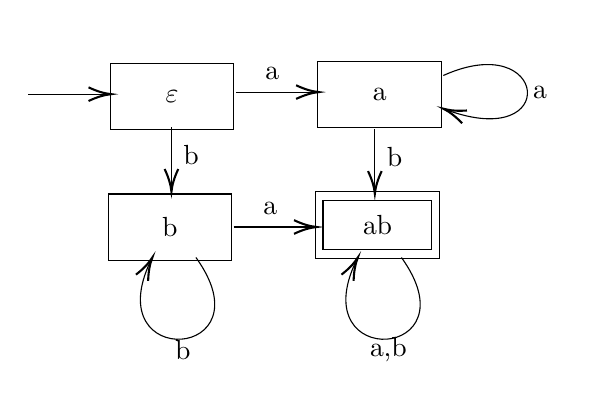
\begin{tikzpicture}[x=0.75pt,y=0.75pt,yscale=-1,xscale=1]
		%uncomment if require: \path (0,273.1999988555908); %set diagram left start at 0, and has height of 273.1999988555908
		
		%Shape: Rectangle [id:dp8492923084975146] 
		\draw   (258,71) -- (317.5,71) -- (317.5,102.91) -- (258,102.91) -- cycle ;
		%Straight Lines [id:da045359006319660056] 
		\draw    (218.5,85.91) -- (256.5,85.91) ;
		\draw [shift={(258.5,85.91)}, rotate = 180] [color={rgb, 255:red, 0; green, 0; blue, 0 }  ][line width=0.75]    (10.93,-3.29) .. controls (6.95,-1.4) and (3.31,-0.3) .. (0,0) .. controls (3.31,0.3) and (6.95,1.4) .. (10.93,3.29)   ;
		
		%Straight Lines [id:da8932931676266114] 
		\draw    (287.5,101.91) -- (287.5,130.91) ;
		\draw [shift={(287.5,132.91)}, rotate = 270] [color={rgb, 255:red, 0; green, 0; blue, 0 }  ][line width=0.75]    (10.93,-3.29) .. controls (6.95,-1.4) and (3.31,-0.3) .. (0,0) .. controls (3.31,0.3) and (6.95,1.4) .. (10.93,3.29)   ;
		
		%Shape: Rectangle [id:dp7060596178969023] 
		\draw   (358,70) -- (417.5,70) -- (417.5,101.91) -- (358,101.91) -- cycle ;
		%Straight Lines [id:da29122783005606534] 
		\draw    (318.5,84.91) -- (356.5,84.91) ;
		\draw [shift={(358.5,84.91)}, rotate = 180] [color={rgb, 255:red, 0; green, 0; blue, 0 }  ][line width=0.75]    (10.93,-3.29) .. controls (6.95,-1.4) and (3.31,-0.3) .. (0,0) .. controls (3.31,0.3) and (6.95,1.4) .. (10.93,3.29)   ;
		
		%Shape: Rectangle [id:dp2569584546249841] 
		\draw   (257,134) -- (316.5,134) -- (316.5,165.91) -- (257,165.91) -- cycle ;
		%Shape: Rectangle [id:dp09010840781538398] 
		\draw   (357,133) -- (416.5,133) -- (416.5,164.91) -- (357,164.91) -- cycle ;
		%Straight Lines [id:da11493138024036909] 
		\draw    (317.5,149.91) -- (355.5,149.91) ;
		\draw [shift={(357.5,149.91)}, rotate = 180] [color={rgb, 255:red, 0; green, 0; blue, 0 }  ][line width=0.75]    (10.93,-3.29) .. controls (6.95,-1.4) and (3.31,-0.3) .. (0,0) .. controls (3.31,0.3) and (6.95,1.4) .. (10.93,3.29)   ;
		
		%Straight Lines [id:da43828934166006217] 
		\draw    (385.5,102.91) -- (385.5,131.91) ;
		\draw [shift={(385.5,133.91)}, rotate = 270] [color={rgb, 255:red, 0; green, 0; blue, 0 }  ][line width=0.75]    (10.93,-3.29) .. controls (6.95,-1.4) and (3.31,-0.3) .. (0,0) .. controls (3.31,0.3) and (6.95,1.4) .. (10.93,3.29)   ;
		
		%Shape: Rectangle [id:dp26691452412251593] 
		\draw   (360.5,137) -- (413,137) -- (413,160.91) -- (360.5,160.91) -- cycle ;
		%Curve Lines [id:da34749791532096563] 
		\draw    (398.3,164.6) .. controls (433.94,214.1) and (350.99,219.5) .. (376.49,166.23) ;
		\draw [shift={(377.3,164.6)}, rotate = 476.98] [color={rgb, 255:red, 0; green, 0; blue, 0 }  ][line width=0.75]    (10.93,-3.29) .. controls (6.95,-1.4) and (3.31,-0.3) .. (0,0) .. controls (3.31,0.3) and (6.95,1.4) .. (10.93,3.29)   ;
		
		%Curve Lines [id:da6747160102388468] 
		\draw    (299.3,164.6) .. controls (334.94,214.1) and (251.99,219.5) .. (277.49,166.23) ;
		\draw [shift={(278.3,164.6)}, rotate = 476.98] [color={rgb, 255:red, 0; green, 0; blue, 0 }  ][line width=0.75]    (10.93,-3.29) .. controls (6.95,-1.4) and (3.31,-0.3) .. (0,0) .. controls (3.31,0.3) and (6.95,1.4) .. (10.93,3.29)   ;
		
		%Curve Lines [id:da8794777581749971] 
		\draw    (418.5,76.91) .. controls (468.99,54.14) and (475.38,113.69) .. (420.19,93.54) ;
		\draw [shift={(418.5,92.91)}, rotate = 381.1] [color={rgb, 255:red, 0; green, 0; blue, 0 }  ][line width=0.75]    (10.93,-3.29) .. controls (6.95,-1.4) and (3.31,-0.3) .. (0,0) .. controls (3.31,0.3) and (6.95,1.4) .. (10.93,3.29)   ;
		
		% Text Node
		\draw (336,76) node  [align=left] {a};
		% Text Node
		\draw (335,141) node  [align=left] {a};
		% Text Node
		\draw (297,115) node  [align=left] {b};
		% Text Node
		\draw (395,116) node  [align=left] {b};
		% Text Node
		\draw (287.75,86.95) node  [align=left] {$\varepsilon$};
		% Text Node
		\draw (387.75,85.95) node  [align=left] {a};
		% Text Node
		\draw (286.75,149.95) node  [align=left] {b};
		% Text Node
		\draw (386.75,148.95) node  [align=left] {ab};
		% Text Node
		\draw (392,209) node  [align=left] {a,b};
		% Text Node
		\draw (293,209) node  [align=left] {b};
		% Text Node
		\draw (465,85) node  [align=left] {a};
		
		\end{tikzpicture}

	\item[(g)]
		L = $\{ \:\{\varepsilon, a, aa, aaa\}, \{a, b\}, \delta, \varepsilon, \{\varepsilon, a, aaa\}\}$	\\
		$\delta = 
		\begin{array}{ c|c|c }
			 & a & b\\
			\hline
			\varepsilon & \varepsilon & a\\
			\hline
			a & a & aa\\
			\hline
			aa & aa & aaa\\
			\hline
			aaa & aaa & aaa
		\end{array}$\\
		
		State diagram:

		\tikzset{every picture/.style={line width=0.75pt}} %set default line width to 0.75pt        
		
		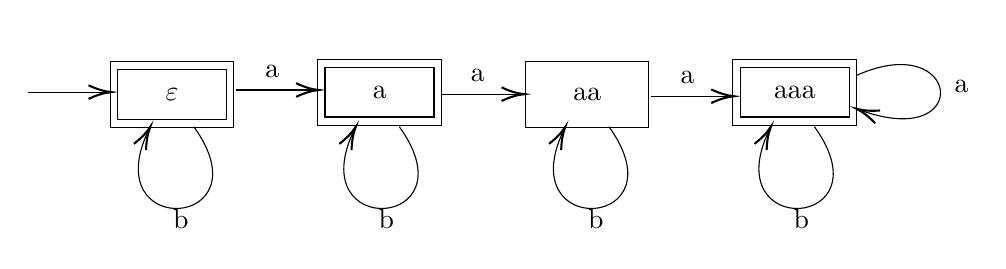
\begin{tikzpicture}[x=0.75pt,y=0.75pt,yscale=-1,xscale=1]
		%uncomment if require: \path (0,273.1999988555908); %set diagram left start at 0, and has height of 273.1999988555908
		
		%Shape: Rectangle [id:dp1526539271886045] 
		\draw   (173,81) -- (232.5,81) -- (232.5,112.91) -- (173,112.91) -- cycle ;
		%Straight Lines [id:da6201993660008029] 
		\draw    (133.5,95.91) -- (171.5,95.91) ;
		\draw [shift={(173.5,95.91)}, rotate = 180] [color={rgb, 255:red, 0; green, 0; blue, 0 }  ][line width=0.75]    (10.93,-3.29) .. controls (6.95,-1.4) and (3.31,-0.3) .. (0,0) .. controls (3.31,0.3) and (6.95,1.4) .. (10.93,3.29)   ;
		
		%Shape: Rectangle [id:dp5926463415832897] 
		\draw   (273,80) -- (332.5,80) -- (332.5,111.91) -- (273,111.91) -- cycle ;
		%Straight Lines [id:da10981659090847451] 
		\draw    (233.5,94.91) -- (271.5,94.91) ;
		\draw [shift={(273.5,94.91)}, rotate = 180] [color={rgb, 255:red, 0; green, 0; blue, 0 }  ][line width=0.75]    (10.93,-3.29) .. controls (6.95,-1.4) and (3.31,-0.3) .. (0,0) .. controls (3.31,0.3) and (6.95,1.4) .. (10.93,3.29)   ;
		
		%Shape: Rectangle [id:dp31965468567794186] 
		\draw   (373,81) -- (432.5,81) -- (432.5,112.91) -- (373,112.91) -- cycle ;
		%Shape: Rectangle [id:dp7032425066303547] 
		\draw   (473,80) -- (532.5,80) -- (532.5,111.91) -- (473,111.91) -- cycle ;
		%Curve Lines [id:da7791756417536615] 
		\draw    (532.5,87.91) .. controls (582.99,65.14) and (589.38,124.69) .. (534.19,104.54) ;
		\draw [shift={(532.5,103.91)}, rotate = 381.1] [color={rgb, 255:red, 0; green, 0; blue, 0 }  ][line width=0.75]    (10.93,-3.29) .. controls (6.95,-1.4) and (3.31,-0.3) .. (0,0) .. controls (3.31,0.3) and (6.95,1.4) .. (10.93,3.29)   ;
		
		%Straight Lines [id:da7582547010652916] 
		\draw    (332.5,96.91) -- (370.5,96.91) ;
		\draw [shift={(372.5,96.91)}, rotate = 180] [color={rgb, 255:red, 0; green, 0; blue, 0 }  ][line width=0.75]    (10.93,-3.29) .. controls (6.95,-1.4) and (3.31,-0.3) .. (0,0) .. controls (3.31,0.3) and (6.95,1.4) .. (10.93,3.29)   ;
		
		%Straight Lines [id:da2846910122415589] 
		\draw    (433.5,97.91) -- (471.5,97.91) ;
		\draw [shift={(473.5,97.91)}, rotate = 180] [color={rgb, 255:red, 0; green, 0; blue, 0 }  ][line width=0.75]    (10.93,-3.29) .. controls (6.95,-1.4) and (3.31,-0.3) .. (0,0) .. controls (3.31,0.3) and (6.95,1.4) .. (10.93,3.29)   ;
		
		%Curve Lines [id:da21283566271184684] 
		\draw    (312.3,112.6) .. controls (347.94,162.1) and (264.99,167.5) .. (290.49,114.23) ;
		\draw [shift={(291.3,112.6)}, rotate = 476.98] [color={rgb, 255:red, 0; green, 0; blue, 0 }  ][line width=0.75]    (10.93,-3.29) .. controls (6.95,-1.4) and (3.31,-0.3) .. (0,0) .. controls (3.31,0.3) and (6.95,1.4) .. (10.93,3.29)   ;
		
		%Curve Lines [id:da16314257404042776] 
		\draw    (213.3,112.6) .. controls (248.94,162.1) and (165.99,167.5) .. (191.49,114.23) ;
		\draw [shift={(192.3,112.6)}, rotate = 476.98] [color={rgb, 255:red, 0; green, 0; blue, 0 }  ][line width=0.75]    (10.93,-3.29) .. controls (6.95,-1.4) and (3.31,-0.3) .. (0,0) .. controls (3.31,0.3) and (6.95,1.4) .. (10.93,3.29)   ;
		
		%Curve Lines [id:da24508950079225178] 
		\draw    (512.3,112.6) .. controls (547.94,162.1) and (464.99,167.5) .. (490.49,114.23) ;
		\draw [shift={(491.3,112.6)}, rotate = 476.98] [color={rgb, 255:red, 0; green, 0; blue, 0 }  ][line width=0.75]    (10.93,-3.29) .. controls (6.95,-1.4) and (3.31,-0.3) .. (0,0) .. controls (3.31,0.3) and (6.95,1.4) .. (10.93,3.29)   ;
		
		%Curve Lines [id:da46438565340790894] 
		\draw    (413.3,112.6) .. controls (448.94,162.1) and (365.99,167.5) .. (391.49,114.23) ;
		\draw [shift={(392.3,112.6)}, rotate = 476.98] [color={rgb, 255:red, 0; green, 0; blue, 0 }  ][line width=0.75]    (10.93,-3.29) .. controls (6.95,-1.4) and (3.31,-0.3) .. (0,0) .. controls (3.31,0.3) and (6.95,1.4) .. (10.93,3.29)   ;
		
		%Shape: Rectangle [id:dp9095754905074096] 
		\draw   (176.5,85) -- (229,85) -- (229,108.91) -- (176.5,108.91) -- cycle ;
		%Shape: Rectangle [id:dp6485129952275841] 
		\draw   (276.5,84) -- (329,84) -- (329,107.91) -- (276.5,107.91) -- cycle ;
		%Shape: Rectangle [id:dp47039216377893767] 
		\draw   (476.5,84) -- (529,84) -- (529,107.91) -- (476.5,107.91) -- cycle ;
		
		% Text Node
		\draw (251,86) node  [align=left] {a};
		% Text Node
		\draw (350,88) node  [align=left] {a};
		% Text Node
		\draw (451,89) node  [align=left] {a};
		% Text Node
		\draw (202.75,96.95) node  [align=left] {$\varepsilon$};
		% Text Node
		\draw (302.75,95.95) node  [align=left] {a};
		% Text Node
		\draw (402.75,96.95) node  [align=left] {aa};
		% Text Node
		\draw (502.75,95.95) node  [align=left] {aaa};
		% Text Node
		\draw (306,157) node  [align=left] {b};
		% Text Node
		\draw (207,157) node  [align=left] {b};
		% Text Node
		\draw (506,157) node  [align=left] {b};
		% Text Node
		\draw (407,157) node  [align=left] {b};
		% Text Node
		\draw (583,93) node  [align=left] {a};
		
		\end{tikzpicture}

	\item[(h)]
		L = $\{ \:\{\varepsilon, a, b, ab\}, \{a, b\}, \delta, \varepsilon, \{\varepsilon, ab\}\}$	\\
		$\delta = 
		\begin{array}{ c|c|c }
			 & a & b\\
			\hline
			\varepsilon & a & b\\
			\hline
			a & ab & ab\\
			\hline
			b & ab & ab
		\end{array}$\\
		
		State diagram:

		\tikzset{every picture/.style={line width=0.75pt}} %set default line width to 0.75pt        
		
		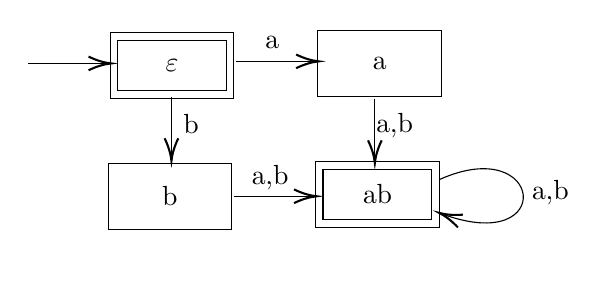
\begin{tikzpicture}[x=0.75pt,y=0.75pt,yscale=-1,xscale=1]
		%uncomment if require: \path (0,273.1999988555908); %set diagram left start at 0, and has height of 273.1999988555908
		
		%Shape: Rectangle [id:dp35389363530061746] 
		\draw   (230,86) -- (289.5,86) -- (289.5,117.91) -- (230,117.91) -- cycle ;
		%Straight Lines [id:da09055196923868514] 
		\draw    (190.5,100.91) -- (228.5,100.91) ;
		\draw [shift={(230.5,100.91)}, rotate = 180] [color={rgb, 255:red, 0; green, 0; blue, 0 }  ][line width=0.75]    (10.93,-3.29) .. controls (6.95,-1.4) and (3.31,-0.3) .. (0,0) .. controls (3.31,0.3) and (6.95,1.4) .. (10.93,3.29)   ;
		
		%Straight Lines [id:da5488463347860157] 
		\draw    (259.5,116.91) -- (259.5,145.91) ;
		\draw [shift={(259.5,147.91)}, rotate = 270] [color={rgb, 255:red, 0; green, 0; blue, 0 }  ][line width=0.75]    (10.93,-3.29) .. controls (6.95,-1.4) and (3.31,-0.3) .. (0,0) .. controls (3.31,0.3) and (6.95,1.4) .. (10.93,3.29)   ;
		
		%Shape: Rectangle [id:dp7732859097177796] 
		\draw   (330,85) -- (389.5,85) -- (389.5,116.91) -- (330,116.91) -- cycle ;
		%Straight Lines [id:da17703370942957597] 
		\draw    (290.5,99.91) -- (328.5,99.91) ;
		\draw [shift={(330.5,99.91)}, rotate = 180] [color={rgb, 255:red, 0; green, 0; blue, 0 }  ][line width=0.75]    (10.93,-3.29) .. controls (6.95,-1.4) and (3.31,-0.3) .. (0,0) .. controls (3.31,0.3) and (6.95,1.4) .. (10.93,3.29)   ;
		
		%Shape: Rectangle [id:dp13394055279353068] 
		\draw   (229,149) -- (288.5,149) -- (288.5,180.91) -- (229,180.91) -- cycle ;
		%Shape: Rectangle [id:dp7799449901531779] 
		\draw   (329,148) -- (388.5,148) -- (388.5,179.91) -- (329,179.91) -- cycle ;
		%Straight Lines [id:da7850466953367499] 
		\draw    (289.5,164.91) -- (327.5,164.91) ;
		\draw [shift={(329.5,164.91)}, rotate = 180] [color={rgb, 255:red, 0; green, 0; blue, 0 }  ][line width=0.75]    (10.93,-3.29) .. controls (6.95,-1.4) and (3.31,-0.3) .. (0,0) .. controls (3.31,0.3) and (6.95,1.4) .. (10.93,3.29)   ;
		
		%Straight Lines [id:da4096284295990671] 
		\draw    (357.5,117.91) -- (357.5,146.91) ;
		\draw [shift={(357.5,148.91)}, rotate = 270] [color={rgb, 255:red, 0; green, 0; blue, 0 }  ][line width=0.75]    (10.93,-3.29) .. controls (6.95,-1.4) and (3.31,-0.3) .. (0,0) .. controls (3.31,0.3) and (6.95,1.4) .. (10.93,3.29)   ;
		
		%Curve Lines [id:da6748246632164858] 
		\draw    (388.5,156.91) .. controls (438.99,134.14) and (445.38,193.69) .. (390.19,173.54) ;
		\draw [shift={(388.5,172.91)}, rotate = 381.1] [color={rgb, 255:red, 0; green, 0; blue, 0 }  ][line width=0.75]    (10.93,-3.29) .. controls (6.95,-1.4) and (3.31,-0.3) .. (0,0) .. controls (3.31,0.3) and (6.95,1.4) .. (10.93,3.29)   ;
		
		%Shape: Rectangle [id:dp8463091498360771] 
		\draw   (332.5,152) -- (385,152) -- (385,175.91) -- (332.5,175.91) -- cycle ;
		%Shape: Rectangle [id:dp7697794753399183] 
		\draw   (233.5,90) -- (286,90) -- (286,113.91) -- (233.5,113.91) -- cycle ;
		
		% Text Node
		\draw (308,91) node  [align=left] {a};
		% Text Node
		\draw (307,156) node  [align=left] {a,b};
		% Text Node
		\draw (269,130) node  [align=left] {b};
		% Text Node
		\draw (367,131) node  [align=left] {a,b};
		% Text Node
		\draw (259.75,101.95) node  [align=left] {$\varepsilon$};
		% Text Node
		\draw (359.75,100.95) node  [align=left] {a};
		% Text Node
		\draw (258.75,164.95) node  [align=left] {b};
		% Text Node
		\draw (358.75,163.95) node  [align=left] {ab};
		% Text Node
		\draw (442,163) node  [align=left] {a,b};
		
		\end{tikzpicture}

\end{enumerate}

\begin{problem}{1.6}
\end{problem}
\begin{enumerate}
	\item[(a)]
		L = $\{ \:\{ \varepsilon, 0, 1, 10, 11\}, \{0, 1\}, \delta, \varepsilon, 10\}$	\\
		$\delta = 
		\begin{array}{ c|c|c }
			 & 0 & 1\\
			\hline
			\varepsilon & 0 & 1\\
			\hline
			0 & 0 & 0\\
			\hline
			1 & 10 & 11\\
			\hline
			10 & 10 & 11\\
			\hline
			11 & 10 & 11
		\end{array}$\\

		State diagram:

		\tikzset{every picture/.style={line width=0.75pt}} %set default line width to 0.75pt        
		
		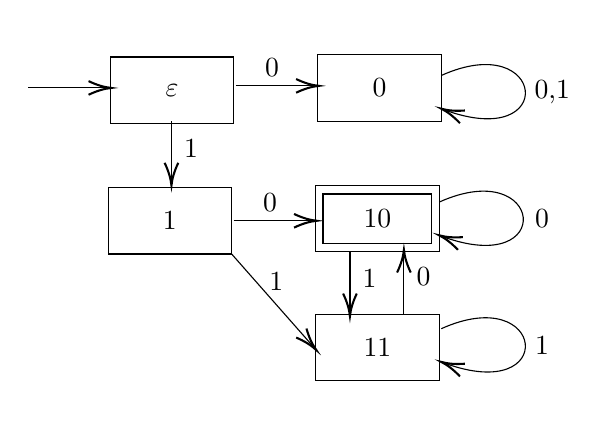
\begin{tikzpicture}[x=0.75pt,y=0.75pt,yscale=-1,xscale=1]
		%uncomment if require: \path (0,273.1999988555908); %set diagram left start at 0, and has height of 273.1999988555908
		
		%Shape: Rectangle [id:dp8093269017049805] 
		\draw   (253,69) -- (312.5,69) -- (312.5,100.91) -- (253,100.91) -- cycle ;
		%Straight Lines [id:da8874354094551611] 
		\draw    (213.5,83.91) -- (251.5,83.91) ;
		\draw [shift={(253.5,83.91)}, rotate = 180] [color={rgb, 255:red, 0; green, 0; blue, 0 }  ][line width=0.75]    (10.93,-3.29) .. controls (6.95,-1.4) and (3.31,-0.3) .. (0,0) .. controls (3.31,0.3) and (6.95,1.4) .. (10.93,3.29)   ;
		
		%Straight Lines [id:da6279578864909225] 
		\draw    (282.5,99.91) -- (282.5,128.91) ;
		\draw [shift={(282.5,130.91)}, rotate = 270] [color={rgb, 255:red, 0; green, 0; blue, 0 }  ][line width=0.75]    (10.93,-3.29) .. controls (6.95,-1.4) and (3.31,-0.3) .. (0,0) .. controls (3.31,0.3) and (6.95,1.4) .. (10.93,3.29)   ;
		
		%Shape: Rectangle [id:dp854516935153814] 
		\draw   (353,68) -- (412.5,68) -- (412.5,99.91) -- (353,99.91) -- cycle ;
		%Straight Lines [id:da84425993362868] 
		\draw    (313.5,82.91) -- (351.5,82.91) ;
		\draw [shift={(353.5,82.91)}, rotate = 180] [color={rgb, 255:red, 0; green, 0; blue, 0 }  ][line width=0.75]    (10.93,-3.29) .. controls (6.95,-1.4) and (3.31,-0.3) .. (0,0) .. controls (3.31,0.3) and (6.95,1.4) .. (10.93,3.29)   ;
		
		%Shape: Rectangle [id:dp2026417483587104] 
		\draw   (252,132) -- (311.5,132) -- (311.5,163.91) -- (252,163.91) -- cycle ;
		%Shape: Rectangle [id:dp056823956455055225] 
		\draw   (352,131) -- (411.5,131) -- (411.5,162.91) -- (352,162.91) -- cycle ;
		%Curve Lines [id:da022280123478476854] 
		\draw    (412.5,77.91) .. controls (462.99,55.14) and (469.38,114.69) .. (414.19,94.54) ;
		\draw [shift={(412.5,93.91)}, rotate = 381.1] [color={rgb, 255:red, 0; green, 0; blue, 0 }  ][line width=0.75]    (10.93,-3.29) .. controls (6.95,-1.4) and (3.31,-0.3) .. (0,0) .. controls (3.31,0.3) and (6.95,1.4) .. (10.93,3.29)   ;
		
		%Straight Lines [id:da3520582938763894] 
		\draw    (312.5,147.91) -- (350.5,147.91) ;
		\draw [shift={(352.5,147.91)}, rotate = 180] [color={rgb, 255:red, 0; green, 0; blue, 0 }  ][line width=0.75]    (10.93,-3.29) .. controls (6.95,-1.4) and (3.31,-0.3) .. (0,0) .. controls (3.31,0.3) and (6.95,1.4) .. (10.93,3.29)   ;
		
		%Shape: Rectangle [id:dp7262989509191828] 
		\draw   (352,193) -- (411.5,193) -- (411.5,224.91) -- (352,224.91) -- cycle ;
		%Straight Lines [id:da5179367785301972] 
		\draw    (311.5,163.91) -- (350.98,208.7) ;
		\draw [shift={(352.3,210.2)}, rotate = 228.61] [color={rgb, 255:red, 0; green, 0; blue, 0 }  ][line width=0.75]    (10.93,-3.29) .. controls (6.95,-1.4) and (3.31,-0.3) .. (0,0) .. controls (3.31,0.3) and (6.95,1.4) .. (10.93,3.29)   ;
		
		%Straight Lines [id:da8207665242865139] 
		\draw    (394.5,163.91) -- (394.5,192.91) ;
		
		\draw [shift={(394.5,161.91)}, rotate = 90] [color={rgb, 255:red, 0; green, 0; blue, 0 }  ][line width=0.75]    (10.93,-3.29) .. controls (6.95,-1.4) and (3.31,-0.3) .. (0,0) .. controls (3.31,0.3) and (6.95,1.4) .. (10.93,3.29)   ;
		%Straight Lines [id:da26400684542065456] 
		\draw    (368.5,162.91) -- (368.5,191.91) ;
		\draw [shift={(368.5,193.91)}, rotate = 270] [color={rgb, 255:red, 0; green, 0; blue, 0 }  ][line width=0.75]    (10.93,-3.29) .. controls (6.95,-1.4) and (3.31,-0.3) .. (0,0) .. controls (3.31,0.3) and (6.95,1.4) .. (10.93,3.29)   ;
		
		%Curve Lines [id:da2907191706671741] 
		\draw    (411.5,138.91) .. controls (461.99,116.14) and (468.38,175.69) .. (413.19,155.54) ;
		\draw [shift={(411.5,154.91)}, rotate = 381.1] [color={rgb, 255:red, 0; green, 0; blue, 0 }  ][line width=0.75]    (10.93,-3.29) .. controls (6.95,-1.4) and (3.31,-0.3) .. (0,0) .. controls (3.31,0.3) and (6.95,1.4) .. (10.93,3.29)   ;
		
		%Curve Lines [id:da4385396734269371] 
		\draw    (412.5,199.91) .. controls (462.99,177.14) and (469.38,236.69) .. (414.19,216.54) ;
		\draw [shift={(412.5,215.91)}, rotate = 381.1] [color={rgb, 255:red, 0; green, 0; blue, 0 }  ][line width=0.75]    (10.93,-3.29) .. controls (6.95,-1.4) and (3.31,-0.3) .. (0,0) .. controls (3.31,0.3) and (6.95,1.4) .. (10.93,3.29)   ;
		
		%Shape: Rectangle [id:dp8824573279948948] 
		\draw   (355.5,135) -- (408,135) -- (408,158.91) -- (355.5,158.91) -- cycle ;
		
		% Text Node
		\draw (331,74) node  [align=left] {0};
		% Text Node
		\draw (330,139) node  [align=left] {0};
		% Text Node
		\draw (466,86) node  [align=left] {0,1};
		% Text Node
		\draw (292,113) node  [align=left] {1};
		% Text Node
		\draw (282.75,84.95) node  [align=left] {$\varepsilon$};
		% Text Node
		\draw (382.75,83.95) node  [align=left] {0};
		% Text Node
		\draw (281.75,147.95) node  [align=left] {1};
		% Text Node
		\draw (381.75,146.95) node  [align=left] {10};
		% Text Node
		\draw (381.75,208.95) node  [align=left] {11};
		% Text Node
		\draw (333,177) node  [align=left] {1};
		% Text Node
		\draw (404,175) node  [align=left] {0};
		% Text Node
		\draw (378,176) node  [align=left] {1};
		% Text Node
		\draw (461,147) node  [align=left] {0};
		% Text Node
		\draw (461,208) node  [align=left] {1};
		
		\end{tikzpicture}

	\item[(b)]
		L = $\{ \:\{ \varepsilon, 1, 11, 111\}, \{0, 1\}, \delta, \varepsilon, 111\}$	\\
		$\delta = 
		\begin{array}{ c|c|c }
			 & 0 & 1\\
			\hline
			\varepsilon & \varepsilon & 1\\
			\hline
			1 & 1 & 11\\
			\hline
			11 & 11 & 111\\
			\hline
			111 & 111 & 111
		\end{array}$\\

		State diagram:

		\tikzset{every picture/.style={line width=0.75pt}} %set default line width to 0.75pt        
		
		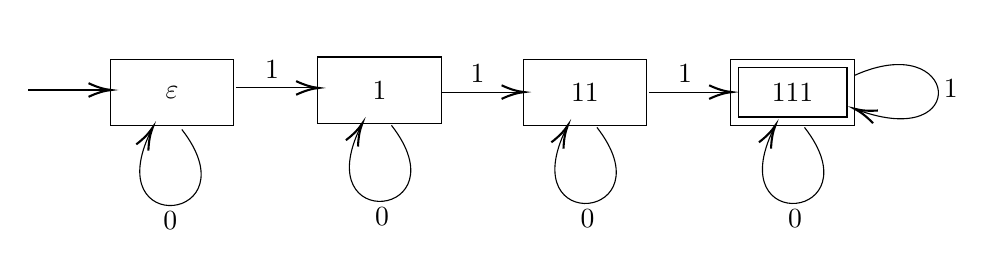
\begin{tikzpicture}[x=0.75pt,y=0.75pt,yscale=-1,xscale=1]
		%uncomment if require: \path (0,273.1999988555908); %set diagram left start at 0, and has height of 273.1999988555908
		
		%Shape: Rectangle [id:dp023052373166507323] 
		\draw   (493.5,60) -- (546,60) -- (546,83.91) -- (493.5,83.91) -- cycle ;
		%Shape: Rectangle [id:dp3270360503209424] 
		\draw   (191,56) -- (250.5,56) -- (250.5,87.91) -- (191,87.91) -- cycle ;
		%Straight Lines [id:da6381520828912002] 
		\draw    (151.5,70.91) -- (189.5,70.91) ;
		\draw [shift={(191.5,70.91)}, rotate = 180] [color={rgb, 255:red, 0; green, 0; blue, 0 }  ][line width=0.75]    (10.93,-3.29) .. controls (6.95,-1.4) and (3.31,-0.3) .. (0,0) .. controls (3.31,0.3) and (6.95,1.4) .. (10.93,3.29)   ;
		
		%Shape: Rectangle [id:dp6168354330830901] 
		\draw   (291,55) -- (350.5,55) -- (350.5,86.91) -- (291,86.91) -- cycle ;
		%Straight Lines [id:da4991120670851208] 
		\draw    (251.5,69.91) -- (289.5,69.91) ;
		\draw [shift={(291.5,69.91)}, rotate = 180] [color={rgb, 255:red, 0; green, 0; blue, 0 }  ][line width=0.75]    (10.93,-3.29) .. controls (6.95,-1.4) and (3.31,-0.3) .. (0,0) .. controls (3.31,0.3) and (6.95,1.4) .. (10.93,3.29)   ;
		
		%Curve Lines [id:da602462258548252] 
		\draw    (549.5,63.91) .. controls (599.99,41.14) and (606.38,100.69) .. (551.19,80.54) ;
		\draw [shift={(549.5,79.91)}, rotate = 381.1] [color={rgb, 255:red, 0; green, 0; blue, 0 }  ][line width=0.75]    (10.93,-3.29) .. controls (6.95,-1.4) and (3.31,-0.3) .. (0,0) .. controls (3.31,0.3) and (6.95,1.4) .. (10.93,3.29)   ;
		
		%Curve Lines [id:da975184156291951] 
		\draw    (225.5,89.91) .. controls (260.15,134.46) and (185.03,142.74) .. (210.69,90.51) ;
		\draw [shift={(211.5,88.91)}, rotate = 477.41] [color={rgb, 255:red, 0; green, 0; blue, 0 }  ][line width=0.75]    (10.93,-3.29) .. controls (6.95,-1.4) and (3.31,-0.3) .. (0,0) .. controls (3.31,0.3) and (6.95,1.4) .. (10.93,3.29)   ;
		
		%Curve Lines [id:da21768429173261006] 
		\draw    (326.5,87.91) .. controls (361.15,132.46) and (286.03,140.74) .. (311.69,88.51) ;
		\draw [shift={(312.5,86.91)}, rotate = 477.41] [color={rgb, 255:red, 0; green, 0; blue, 0 }  ][line width=0.75]    (10.93,-3.29) .. controls (6.95,-1.4) and (3.31,-0.3) .. (0,0) .. controls (3.31,0.3) and (6.95,1.4) .. (10.93,3.29)   ;
		
		%Shape: Rectangle [id:dp3395778654029553] 
		\draw   (390,56) -- (449.5,56) -- (449.5,87.91) -- (390,87.91) -- cycle ;
		%Straight Lines [id:da4132967149828106] 
		\draw    (350.5,71.91) -- (388.5,71.91) ;
		\draw [shift={(390.5,71.91)}, rotate = 180] [color={rgb, 255:red, 0; green, 0; blue, 0 }  ][line width=0.75]    (10.93,-3.29) .. controls (6.95,-1.4) and (3.31,-0.3) .. (0,0) .. controls (3.31,0.3) and (6.95,1.4) .. (10.93,3.29)   ;
		
		%Curve Lines [id:da27093691209549875] 
		\draw    (425.5,88.91) .. controls (460.15,133.46) and (385.03,141.74) .. (410.69,89.51) ;
		\draw [shift={(411.5,87.91)}, rotate = 477.41] [color={rgb, 255:red, 0; green, 0; blue, 0 }  ][line width=0.75]    (10.93,-3.29) .. controls (6.95,-1.4) and (3.31,-0.3) .. (0,0) .. controls (3.31,0.3) and (6.95,1.4) .. (10.93,3.29)   ;
		
		%Shape: Rectangle [id:dp12831521739996332] 
		\draw   (490,56) -- (549.5,56) -- (549.5,87.91) -- (490,87.91) -- cycle ;
		%Straight Lines [id:da956584794339526] 
		\draw    (450.5,71.91) -- (488.5,71.91) ;
		\draw [shift={(490.5,71.91)}, rotate = 180] [color={rgb, 255:red, 0; green, 0; blue, 0 }  ][line width=0.75]    (10.93,-3.29) .. controls (6.95,-1.4) and (3.31,-0.3) .. (0,0) .. controls (3.31,0.3) and (6.95,1.4) .. (10.93,3.29)   ;
		
		%Curve Lines [id:da7430838990900566] 
		\draw    (525.5,88.91) .. controls (560.15,133.46) and (485.03,141.74) .. (510.69,89.51) ;
		\draw [shift={(511.5,87.91)}, rotate = 477.41] [color={rgb, 255:red, 0; green, 0; blue, 0 }  ][line width=0.75]    (10.93,-3.29) .. controls (6.95,-1.4) and (3.31,-0.3) .. (0,0) .. controls (3.31,0.3) and (6.95,1.4) .. (10.93,3.29)   ;
		
		% Text Node
		\draw (269,61) node  [align=left] {1};
		% Text Node
		\draw (596,70) node  [align=left] {1};
		% Text Node
		\draw (220,134) node  [align=left] {0};
		% Text Node
		\draw (322,132) node  [align=left] {0};
		% Text Node
		\draw (220.75,71.95) node  [align=left] {$\varepsilon$};
		% Text Node
		\draw (320.75,70.95) node  [align=left] {1};
		% Text Node
		\draw (368,63) node  [align=left] {1};
		% Text Node
		\draw (421,133) node  [align=left] {0};
		% Text Node
		\draw (419.75,71.95) node  [align=left] {11};
		% Text Node
		\draw (468,63) node  [align=left] {1};
		% Text Node
		\draw (521,133) node  [align=left] {0};
		% Text Node
		\draw (519.75,71.95) node  [align=left] {111};
		
		\end{tikzpicture}

	\item[(c)]
		L = $\{ \:\{ \varepsilon, 0, 01, 010, 0101\}, \{0, 1\}, \delta, \varepsilon, 0101\}$	\\
		$\delta = 
		\begin{array}{ c|c|c }
			 & 0 & 1\\
			\hline
			\varepsilon & 0 & \varepsilon\\
			\hline
			0 & 0 & 01\\
			\hline
			01 & 010 & \varepsilon\\
			\hline
			010 & 0 & 0101\\
			\hline
			0101 & 0101 & 0101
		\end{array}$\\

		State diagram:

		\tikzset{every picture/.style={line width=0.75pt}} %set default line width to 0.75pt        
		
		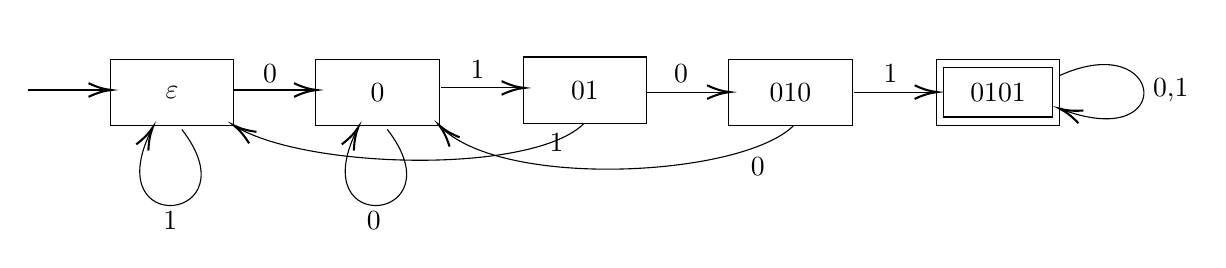
\begin{tikzpicture}[x=0.75pt,y=0.75pt,yscale=-1,xscale=1]
		%uncomment if require: \path (0,273.1999988555908); %set diagram left start at 0, and has height of 273.1999988555908
		
		%Shape: Rectangle [id:dp956976788795576] 
		\draw   (493.5,60) -- (546,60) -- (546,83.91) -- (493.5,83.91) -- cycle ;
		%Shape: Rectangle [id:dp8420859467362585] 
		\draw   (191,56) -- (250.5,56) -- (250.5,87.91) -- (191,87.91) -- cycle ;
		%Straight Lines [id:da5058522979107305] 
		\draw    (151.5,70.91) -- (189.5,70.91) ;
		\draw [shift={(191.5,70.91)}, rotate = 180] [color={rgb, 255:red, 0; green, 0; blue, 0 }  ][line width=0.75]    (10.93,-3.29) .. controls (6.95,-1.4) and (3.31,-0.3) .. (0,0) .. controls (3.31,0.3) and (6.95,1.4) .. (10.93,3.29)   ;
		
		%Shape: Rectangle [id:dp14240592094191928] 
		\draw   (291,55) -- (350.5,55) -- (350.5,86.91) -- (291,86.91) -- cycle ;
		%Straight Lines [id:da8400508696340678] 
		\draw    (251.5,69.91) -- (289.5,69.91) ;
		\draw [shift={(291.5,69.91)}, rotate = 180] [color={rgb, 255:red, 0; green, 0; blue, 0 }  ][line width=0.75]    (10.93,-3.29) .. controls (6.95,-1.4) and (3.31,-0.3) .. (0,0) .. controls (3.31,0.3) and (6.95,1.4) .. (10.93,3.29)   ;
		
		%Curve Lines [id:da3929647914483967] 
		\draw    (549.5,63.91) .. controls (599.99,41.14) and (606.38,100.69) .. (551.19,80.54) ;
		\draw [shift={(549.5,79.91)}, rotate = 381.1] [color={rgb, 255:red, 0; green, 0; blue, 0 }  ][line width=0.75]    (10.93,-3.29) .. controls (6.95,-1.4) and (3.31,-0.3) .. (0,0) .. controls (3.31,0.3) and (6.95,1.4) .. (10.93,3.29)   ;
		
		%Curve Lines [id:da43209873002088006] 
		\draw    (225.5,89.91) .. controls (260.15,134.46) and (185.03,142.74) .. (210.69,90.51) ;
		\draw [shift={(211.5,88.91)}, rotate = 477.41] [color={rgb, 255:red, 0; green, 0; blue, 0 }  ][line width=0.75]    (10.93,-3.29) .. controls (6.95,-1.4) and (3.31,-0.3) .. (0,0) .. controls (3.31,0.3) and (6.95,1.4) .. (10.93,3.29)   ;
		
		%Shape: Rectangle [id:dp9254601209026325] 
		\draw   (390,56) -- (449.5,56) -- (449.5,87.91) -- (390,87.91) -- cycle ;
		%Straight Lines [id:da5368673556619235] 
		\draw    (350.5,71.91) -- (388.5,71.91) ;
		\draw [shift={(390.5,71.91)}, rotate = 180] [color={rgb, 255:red, 0; green, 0; blue, 0 }  ][line width=0.75]    (10.93,-3.29) .. controls (6.95,-1.4) and (3.31,-0.3) .. (0,0) .. controls (3.31,0.3) and (6.95,1.4) .. (10.93,3.29)   ;
		
		%Shape: Rectangle [id:dp09868809673865675] 
		\draw   (490,56) -- (549.5,56) -- (549.5,87.91) -- (490,87.91) -- cycle ;
		%Straight Lines [id:da5198608402177753] 
		\draw    (450.5,71.91) -- (488.5,71.91) ;
		\draw [shift={(490.5,71.91)}, rotate = 180] [color={rgb, 255:red, 0; green, 0; blue, 0 }  ][line width=0.75]    (10.93,-3.29) .. controls (6.95,-1.4) and (3.31,-0.3) .. (0,0) .. controls (3.31,0.3) and (6.95,1.4) .. (10.93,3.29)   ;
		
		%Curve Lines [id:da16178621977035013] 
		\draw    (320.3,87) .. controls (295.67,111.63) and (187.61,109.08) .. (153.03,88.84) ;
		\draw [shift={(151.5,87.91)}, rotate = 392.75] [color={rgb, 255:red, 0; green, 0; blue, 0 }  ][line width=0.75]    (10.93,-3.29) .. controls (6.95,-1.4) and (3.31,-0.3) .. (0,0) .. controls (3.31,0.3) and (6.95,1.4) .. (10.93,3.29)   ;
		
		%Curve Lines [id:da38464073621417727] 
		\draw    (421.3,88) .. controls (396.67,112.63) and (282.79,118.82) .. (251.85,89.28) ;
		\draw [shift={(250.5,87.91)}, rotate = 407.19] [color={rgb, 255:red, 0; green, 0; blue, 0 }  ][line width=0.75]    (10.93,-3.29) .. controls (6.95,-1.4) and (3.31,-0.3) .. (0,0) .. controls (3.31,0.3) and (6.95,1.4) .. (10.93,3.29)   ;
		
		%Shape: Rectangle [id:dp7772611499680067] 
		\draw   (92,56) -- (151.5,56) -- (151.5,87.91) -- (92,87.91) -- cycle ;
		%Straight Lines [id:da3541280054643685] 
		\draw    (52.5,70.91) -- (90.5,70.91) ;
		\draw [shift={(92.5,70.91)}, rotate = 180] [color={rgb, 255:red, 0; green, 0; blue, 0 }  ][line width=0.75]    (10.93,-3.29) .. controls (6.95,-1.4) and (3.31,-0.3) .. (0,0) .. controls (3.31,0.3) and (6.95,1.4) .. (10.93,3.29)   ;
		
		%Curve Lines [id:da38525068704112164] 
		\draw    (126.5,89.91) .. controls (161.15,134.46) and (86.03,142.74) .. (111.69,90.51) ;
		\draw [shift={(112.5,88.91)}, rotate = 477.41] [color={rgb, 255:red, 0; green, 0; blue, 0 }  ][line width=0.75]    (10.93,-3.29) .. controls (6.95,-1.4) and (3.31,-0.3) .. (0,0) .. controls (3.31,0.3) and (6.95,1.4) .. (10.93,3.29)   ;
		
		% Text Node
		\draw (269,61) node  [align=left] {1};
		% Text Node
		\draw (603,71) node  [align=left] {0,1};
		% Text Node
		\draw (219,134) node  [align=left] {0};
		% Text Node
		\draw (220.75,71.95) node  [align=left] {0};
		% Text Node
		\draw (320.75,70.95) node  [align=left] {01};
		% Text Node
		\draw (367,63) node  [align=left] {0};
		% Text Node
		\draw (419.75,71.95) node  [align=left] {010};
		% Text Node
		\draw (468,63) node  [align=left] {1};
		% Text Node
		\draw (519.75,71.95) node  [align=left] {0101};
		% Text Node
		\draw (307,96) node  [align=left] {1};
		% Text Node
		\draw (404,108) node  [align=left] {0};
		% Text Node
		\draw (121,134) node  [align=left] {1};
		% Text Node
		\draw (121.75,71.95) node  [align=left] {$\varepsilon$};
		% Text Node
		\draw (169,63) node  [align=left] {0};
		
		\end{tikzpicture}

	\item[(d)]
		L = $\{ \:\{ \varepsilon, q1, q2, q3, q4\}, \{0, 1\}, \delta, \varepsilon, q3\}$	\\
		$\delta = 
		\begin{array}{ c|c|c }
			 & 0 & 1\\
			\hline
			\varepsilon & q1 & q1\\
			\hline
			q1 & q2 & q2\\
			\hline
			q2 & q3 & q4\\
			\hline
			q3 & q3 & q3\\
			\hline
			q4 & q4 & q4
		\end{array}$\\

		State diagram:

		\tikzset{every picture/.style={line width=0.75pt}} %set default line width to 0.75pt        
		
		\begin{tikzpicture}[x=0.75pt,y=0.75pt,yscale=-1,xscale=1]
		%uncomment if require: \path (0,273.1999988555908); %set diagram left start at 0, and has height of 273.1999988555908
		
		%Shape: Rectangle [id:dp5393584641890483] 
		\draw   (393.5,60) -- (446,60) -- (446,83.91) -- (393.5,83.91) -- cycle ;
		%Shape: Rectangle [id:dp8433476551815908] 
		\draw   (191,56) -- (250.5,56) -- (250.5,87.91) -- (191,87.91) -- cycle ;
		%Straight Lines [id:da4076229161938647] 
		\draw    (151.5,70.91) -- (189.5,70.91) ;
		\draw [shift={(191.5,70.91)}, rotate = 180] [color={rgb, 255:red, 0; green, 0; blue, 0 }  ][line width=0.75]    (10.93,-3.29) .. controls (6.95,-1.4) and (3.31,-0.3) .. (0,0) .. controls (3.31,0.3) and (6.95,1.4) .. (10.93,3.29)   ;
		
		%Shape: Rectangle [id:dp15204234109882364] 
		\draw   (291,55) -- (350.5,55) -- (350.5,86.91) -- (291,86.91) -- cycle ;
		%Straight Lines [id:da6228583835877859] 
		\draw    (251.5,69.91) -- (289.5,69.91) ;
		\draw [shift={(291.5,69.91)}, rotate = 180] [color={rgb, 255:red, 0; green, 0; blue, 0 }  ][line width=0.75]    (10.93,-3.29) .. controls (6.95,-1.4) and (3.31,-0.3) .. (0,0) .. controls (3.31,0.3) and (6.95,1.4) .. (10.93,3.29)   ;
		
		%Curve Lines [id:da5164575863915815] 
		\draw    (449.5,63.91) .. controls (499.99,41.14) and (506.38,100.69) .. (451.19,80.54) ;
		\draw [shift={(449.5,79.91)}, rotate = 381.1] [color={rgb, 255:red, 0; green, 0; blue, 0 }  ][line width=0.75]    (10.93,-3.29) .. controls (6.95,-1.4) and (3.31,-0.3) .. (0,0) .. controls (3.31,0.3) and (6.95,1.4) .. (10.93,3.29)   ;
		
		%Shape: Rectangle [id:dp979264153701048] 
		\draw   (390,56) -- (449.5,56) -- (449.5,87.91) -- (390,87.91) -- cycle ;
		%Straight Lines [id:da23215527948453896] 
		\draw    (350.5,71.91) -- (388.5,71.91) ;
		\draw [shift={(390.5,71.91)}, rotate = 180] [color={rgb, 255:red, 0; green, 0; blue, 0 }  ][line width=0.75]    (10.93,-3.29) .. controls (6.95,-1.4) and (3.31,-0.3) .. (0,0) .. controls (3.31,0.3) and (6.95,1.4) .. (10.93,3.29)   ;
		
		%Shape: Rectangle [id:dp44010297154680145] 
		\draw   (92,56) -- (151.5,56) -- (151.5,87.91) -- (92,87.91) -- cycle ;
		%Straight Lines [id:da3196333456912812] 
		\draw    (52.5,70.91) -- (90.5,70.91) ;
		\draw [shift={(92.5,70.91)}, rotate = 180] [color={rgb, 255:red, 0; green, 0; blue, 0 }  ][line width=0.75]    (10.93,-3.29) .. controls (6.95,-1.4) and (3.31,-0.3) .. (0,0) .. controls (3.31,0.3) and (6.95,1.4) .. (10.93,3.29)   ;
		
		%Straight Lines [id:da7400584584663139] 
		\draw    (320.5,86.91) -- (320.5,115.91) ;
		\draw [shift={(320.5,117.91)}, rotate = 270] [color={rgb, 255:red, 0; green, 0; blue, 0 }  ][line width=0.75]    (10.93,-3.29) .. controls (6.95,-1.4) and (3.31,-0.3) .. (0,0) .. controls (3.31,0.3) and (6.95,1.4) .. (10.93,3.29)   ;
		
		%Shape: Rectangle [id:dp06122631651578381] 
		\draw   (290,119) -- (349.5,119) -- (349.5,150.91) -- (290,150.91) -- cycle ;
		%Curve Lines [id:da21135169489482908] 
		\draw    (327.5,150.91) .. controls (362.15,195.46) and (287.03,203.74) .. (312.69,151.51) ;
		\draw [shift={(313.5,149.91)}, rotate = 477.41] [color={rgb, 255:red, 0; green, 0; blue, 0 }  ][line width=0.75]    (10.93,-3.29) .. controls (6.95,-1.4) and (3.31,-0.3) .. (0,0) .. controls (3.31,0.3) and (6.95,1.4) .. (10.93,3.29)   ;
		
		% Text Node
		\draw (269,61) node  [align=left] {0,1};
		% Text Node
		\draw (503,71) node  [align=left] {0,1};
		% Text Node
		\draw (220.75,71.95) node  [align=left] {q1};
		% Text Node
		\draw (320.75,70.95) node  [align=left] {q2};
		% Text Node
		\draw (367,63) node  [align=left] {0};
		% Text Node
		\draw (419.75,71.95) node  [align=left] {q3};
		% Text Node
		\draw (121.75,71.95) node  [align=left] {$\varepsilon$};
		% Text Node
		\draw (169,63) node  [align=left] {0,1};
		% Text Node
		\draw (330,100) node  [align=left] {1};
		% Text Node
		\draw (322,195) node  [align=left] {0,1};
		% Text Node
		\draw (319.75,134.95) node  [align=left] {q4};

		\end{tikzpicture}

	\item[(e)]	
		L = $\{ \:\{ \varepsilon, 0, 1,q0, q1\}, \{0, 1\}, \delta, \varepsilon, \{0, q1\}\}$	\\
		$\delta = 
		\begin{array}{ c|c|c }
			 & 0 & 1\\
			\hline
			\varepsilon & 0 & 1\\
			\hline
			0 & q0 & q0\\
			\hline
			1 & q1 & q1\\
			\hline
			q0 & 0 & 0\\
			\hline
			q1 & 1 & 1
		\end{array}$\\

		State diagram:

		\tikzset{every picture/.style={line width=0.75pt}} %set default line width to 0.75pt        
		
		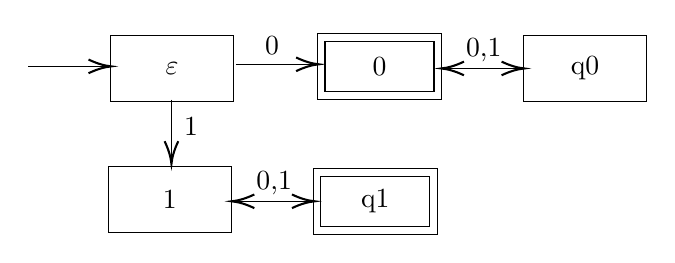
\begin{tikzpicture}[x=0.75pt,y=0.75pt,yscale=-1,xscale=1]
		%uncomment if require: \path (0,273.1999988555908); %set diagram left start at 0, and has height of 273.1999988555908
		
		%Shape: Rectangle [id:dp7239117135107249] 
		\draw   (176,55) -- (235.5,55) -- (235.5,86.91) -- (176,86.91) -- cycle ;
		%Straight Lines [id:da099052867647492] 
		\draw    (136.5,69.91) -- (174.5,69.91) ;
		\draw [shift={(176.5,69.91)}, rotate = 180] [color={rgb, 255:red, 0; green, 0; blue, 0 }  ][line width=0.75]    (10.93,-3.29) .. controls (6.95,-1.4) and (3.31,-0.3) .. (0,0) .. controls (3.31,0.3) and (6.95,1.4) .. (10.93,3.29)   ;
		
		%Straight Lines [id:da9379752055223549] 
		\draw    (205.5,85.91) -- (205.5,114.91) ;
		\draw [shift={(205.5,116.91)}, rotate = 270] [color={rgb, 255:red, 0; green, 0; blue, 0 }  ][line width=0.75]    (10.93,-3.29) .. controls (6.95,-1.4) and (3.31,-0.3) .. (0,0) .. controls (3.31,0.3) and (6.95,1.4) .. (10.93,3.29)   ;
		
		%Shape: Rectangle [id:dp7005254449640419] 
		\draw   (276,54) -- (335.5,54) -- (335.5,85.91) -- (276,85.91) -- cycle ;
		%Straight Lines [id:da581492762819964] 
		\draw    (236.5,68.91) -- (274.5,68.91) ;
		\draw [shift={(276.5,68.91)}, rotate = 180] [color={rgb, 255:red, 0; green, 0; blue, 0 }  ][line width=0.75]    (10.93,-3.29) .. controls (6.95,-1.4) and (3.31,-0.3) .. (0,0) .. controls (3.31,0.3) and (6.95,1.4) .. (10.93,3.29)   ;
		
		%Shape: Rectangle [id:dp6512724762739024] 
		\draw   (175,118) -- (234.5,118) -- (234.5,149.91) -- (175,149.91) -- cycle ;
		%Shape: Rectangle [id:dp22658036690380068] 
		\draw   (375,55) -- (434.5,55) -- (434.5,86.91) -- (375,86.91) -- cycle ;
		%Straight Lines [id:da5265863852285189] 
		\draw    (337.5,70.91) -- (373.5,70.91) ;
		\draw [shift={(375.5,70.91)}, rotate = 180] [color={rgb, 255:red, 0; green, 0; blue, 0 }  ][line width=0.75]    (10.93,-3.29) .. controls (6.95,-1.4) and (3.31,-0.3) .. (0,0) .. controls (3.31,0.3) and (6.95,1.4) .. (10.93,3.29)   ;
		\draw [shift={(335.5,70.91)}, rotate = 0] [color={rgb, 255:red, 0; green, 0; blue, 0 }  ][line width=0.75]    (10.93,-3.29) .. controls (6.95,-1.4) and (3.31,-0.3) .. (0,0) .. controls (3.31,0.3) and (6.95,1.4) .. (10.93,3.29)   ;
		%Shape: Rectangle [id:dp5350763604293245] 
		\draw   (279.5,58) -- (332,58) -- (332,81.91) -- (279.5,81.91) -- cycle ;
		%Shape: Rectangle [id:dp7925237835364931] 
		\draw   (274,119) -- (333.5,119) -- (333.5,150.91) -- (274,150.91) -- cycle ;
		%Straight Lines [id:da27993598948726905] 
		\draw    (236.5,134.91) -- (272.5,134.91) ;
		\draw [shift={(274.5,134.91)}, rotate = 180] [color={rgb, 255:red, 0; green, 0; blue, 0 }  ][line width=0.75]    (10.93,-3.29) .. controls (6.95,-1.4) and (3.31,-0.3) .. (0,0) .. controls (3.31,0.3) and (6.95,1.4) .. (10.93,3.29)   ;
		\draw [shift={(234.5,134.91)}, rotate = 0] [color={rgb, 255:red, 0; green, 0; blue, 0 }  ][line width=0.75]    (10.93,-3.29) .. controls (6.95,-1.4) and (3.31,-0.3) .. (0,0) .. controls (3.31,0.3) and (6.95,1.4) .. (10.93,3.29)   ;
		%Shape: Rectangle [id:dp061576511429808134] 
		\draw   (277.5,123) -- (330,123) -- (330,146.91) -- (277.5,146.91) -- cycle ;
		
		% Text Node
		\draw (254,60) node  [align=left] {0};
		% Text Node
		\draw (215,99) node  [align=left] {1};
		% Text Node
		\draw (205.75,70.95) node  [align=left] {$\varepsilon$};
		% Text Node
		\draw (305.75,69.95) node  [align=left] {0};
		% Text Node
		\draw (204.75,133.95) node  [align=left] {1};
		% Text Node
		\draw (356,62) node  [align=left] {0,1};
		% Text Node
		\draw (404.75,70.95) node  [align=left] {q0};
		% Text Node
		\draw (255,126) node  [align=left] {0,1};
		% Text Node
		\draw (303.75,134.95) node  [align=left] {q1};
		
		\end{tikzpicture}

	\item[(f)]
		L = $\{ \:\{ \varepsilon, 1, 11, 110\}, \{0, 1\}, \delta, \varepsilon, \{ \varepsilon, 1, 11\}\}$	\\
		$\delta = 
			\begin{array}{ c|c|c }
			 & 0 & 1\\
			\hline
			\varepsilon & \varepsilon & 1\\
			\hline
			1 & \varepsilon & 11\\
			\hline
			11 & 110 & 11\\
			\hline
			110 & 110 & 110
		\end{array}$\\

		State diagram:

		\tikzset{every picture/.style={line width=0.75pt}} %set default line width to 0.75pt        
		
		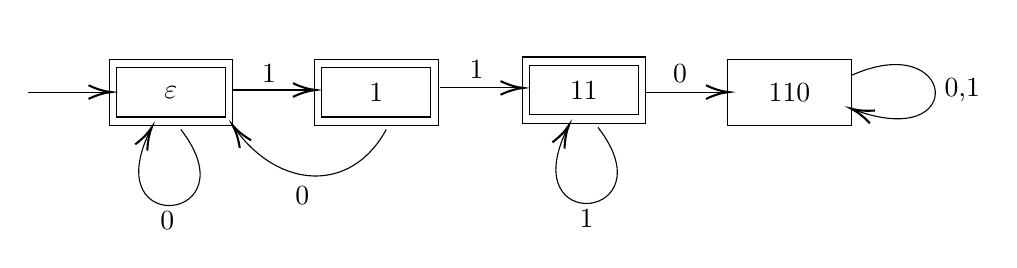
\begin{tikzpicture}[x=0.75pt,y=0.75pt,yscale=-1,xscale=1]
		%uncomment if require: \path (0,273.1999988555908); %set diagram left start at 0, and has height of 273.1999988555908
		
		%Shape: Rectangle [id:dp1513525151412558] 
		\draw   (421.5,80) -- (474,80) -- (474,103.91) -- (421.5,103.91) -- cycle ;
		%Shape: Rectangle [id:dp02460458870090454] 
		\draw   (318,77) -- (377.5,77) -- (377.5,108.91) -- (318,108.91) -- cycle ;
		%Straight Lines [id:da9579026097872703] 
		\draw    (278.5,91.91) -- (316.5,91.91) ;
		\draw [shift={(318.5,91.91)}, rotate = 180] [color={rgb, 255:red, 0; green, 0; blue, 0 }  ][line width=0.75]    (10.93,-3.29) .. controls (6.95,-1.4) and (3.31,-0.3) .. (0,0) .. controls (3.31,0.3) and (6.95,1.4) .. (10.93,3.29)   ;
		
		%Shape: Rectangle [id:dp8612452964581319] 
		\draw   (418,76) -- (477.5,76) -- (477.5,107.91) -- (418,107.91) -- cycle ;
		%Straight Lines [id:da2317125881419888] 
		\draw    (378.5,90.91) -- (416.5,90.91) ;
		\draw [shift={(418.5,90.91)}, rotate = 180] [color={rgb, 255:red, 0; green, 0; blue, 0 }  ][line width=0.75]    (10.93,-3.29) .. controls (6.95,-1.4) and (3.31,-0.3) .. (0,0) .. controls (3.31,0.3) and (6.95,1.4) .. (10.93,3.29)   ;
		
		%Curve Lines [id:da855662850735581] 
		\draw    (352.5,110.91) .. controls (335.56,142.12) and (300.38,139.68) .. (279.45,110.27) ;
		\draw [shift={(278.5,108.91)}, rotate = 415.88] [color={rgb, 255:red, 0; green, 0; blue, 0 }  ][line width=0.75]    (10.93,-3.29) .. controls (6.95,-1.4) and (3.31,-0.3) .. (0,0) .. controls (3.31,0.3) and (6.95,1.4) .. (10.93,3.29)   ;
		
		%Shape: Rectangle [id:dp00036333514892916696] 
		\draw   (517,77) -- (576.5,77) -- (576.5,108.91) -- (517,108.91) -- cycle ;
		%Straight Lines [id:da5984678576608835] 
		\draw    (477.5,92.91) -- (515.5,92.91) ;
		\draw [shift={(517.5,92.91)}, rotate = 180] [color={rgb, 255:red, 0; green, 0; blue, 0 }  ][line width=0.75]    (10.93,-3.29) .. controls (6.95,-1.4) and (3.31,-0.3) .. (0,0) .. controls (3.31,0.3) and (6.95,1.4) .. (10.93,3.29)   ;
		
		%Shape: Rectangle [id:dp9093210601816626] 
		\draw   (219,77) -- (278.5,77) -- (278.5,108.91) -- (219,108.91) -- cycle ;
		%Curve Lines [id:da4915456919405574] 
		\draw    (253.5,110.91) .. controls (288.15,155.46) and (213.03,163.74) .. (238.69,111.51) ;
		\draw [shift={(239.5,109.91)}, rotate = 477.41] [color={rgb, 255:red, 0; green, 0; blue, 0 }  ][line width=0.75]    (10.93,-3.29) .. controls (6.95,-1.4) and (3.31,-0.3) .. (0,0) .. controls (3.31,0.3) and (6.95,1.4) .. (10.93,3.29)   ;
		
		%Curve Lines [id:da8964598834907833] 
		\draw    (576.5,84.91) .. controls (626.99,62.14) and (633.38,121.69) .. (578.19,101.54) ;
		\draw [shift={(576.5,100.91)}, rotate = 381.1] [color={rgb, 255:red, 0; green, 0; blue, 0 }  ][line width=0.75]    (10.93,-3.29) .. controls (6.95,-1.4) and (3.31,-0.3) .. (0,0) .. controls (3.31,0.3) and (6.95,1.4) .. (10.93,3.29)   ;
		
		%Curve Lines [id:da77582925239431] 
		\draw    (454.5,109.91) .. controls (489.15,154.46) and (414.03,162.74) .. (439.69,110.51) ;
		\draw [shift={(440.5,108.91)}, rotate = 477.41] [color={rgb, 255:red, 0; green, 0; blue, 0 }  ][line width=0.75]    (10.93,-3.29) .. controls (6.95,-1.4) and (3.31,-0.3) .. (0,0) .. controls (3.31,0.3) and (6.95,1.4) .. (10.93,3.29)   ;
		
		%Straight Lines [id:da22915732216063733] 
		\draw    (180,92.91) -- (218,92.91) ;
		\draw [shift={(220,92.91)}, rotate = 180] [color={rgb, 255:red, 0; green, 0; blue, 0 }  ][line width=0.75]    (10.93,-3.29) .. controls (6.95,-1.4) and (3.31,-0.3) .. (0,0) .. controls (3.31,0.3) and (6.95,1.4) .. (10.93,3.29)   ;
		
		%Shape: Rectangle [id:dp6160841032292648] 
		\draw   (321.5,81) -- (374,81) -- (374,104.91) -- (321.5,104.91) -- cycle ;
		%Shape: Rectangle [id:dp9681586353297968] 
		\draw   (222.5,81) -- (275,81) -- (275,104.91) -- (222.5,104.91) -- cycle ;
		
		% Text Node
		\draw (396,82) node  [align=left] {1};
		% Text Node
		\draw (347.75,92.95) node  [align=left] {1};
		% Text Node
		\draw (447.75,91.95) node  [align=left] {11};
		% Text Node
		\draw (494,84) node  [align=left] {0};
		% Text Node
		\draw (546.75,92.95) node  [align=left] {110};
		% Text Node
		\draw (248.75,92.95) node  [align=left] {$\varepsilon$};
		% Text Node
		\draw (296,84) node  [align=left] {1};
		% Text Node
		\draw (247,155) node  [align=left] {0};
		% Text Node
		\draw (312,143) node  [align=left] {0};
		% Text Node
		\draw (630,92) node  [align=left] {0,1};
		% Text Node
		\draw (449,154) node  [align=left] {1};
		
		\end{tikzpicture}

	\item[(g)]
		L = $\{ \:\{ \varepsilon, q1,q2,q3,q4,q5,q6\}, \{0, 1\}, \delta, \varepsilon, \{ \varepsilon, q1,q2,q3,q4,q5\}\}$	\\
		$\delta = 
			\begin{array}{ c|c|c }
			 & 0 & 1\\
			\hline
			\varepsilon & q1 & q1\\
			\hline
			q1 & q2 & q2\\
			\hline
			q2 & q3 & q3\\
			\hline
			q3 & q4 & q4\\
			\hline
			q4 & q5 & q5\\
			\hline
			q5 & q6 & q6\\
			\hline
			q6 & q6 & q6
		\end{array}$\\

		State diagram:

		\tikzset{every picture/.style={line width=0.75pt}} %set default line width to 0.75pt        
		
		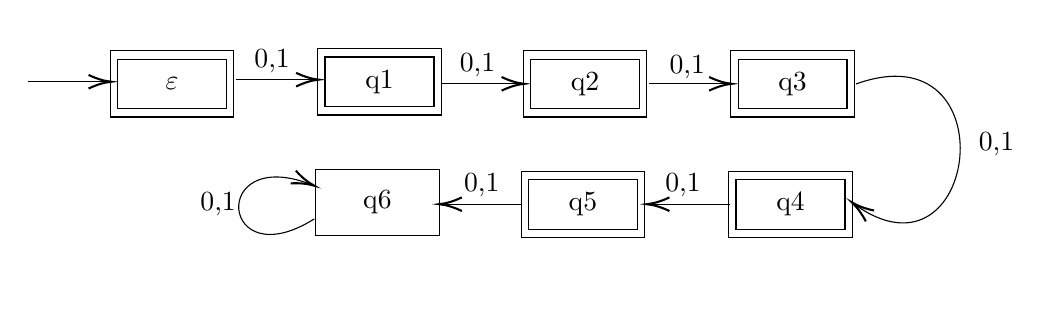
\begin{tikzpicture}[x=0.75pt,y=0.75pt,yscale=-1,xscale=1]
		%uncomment if require: \path (0,273.1999988555908); %set diagram left start at 0, and has height of 273.1999988555908
		
		%Shape: Rectangle [id:dp33729057224007164] 
		\draw   (128,42) -- (187.5,42) -- (187.5,73.91) -- (128,73.91) -- cycle ;
		%Straight Lines [id:da28462577111262033] 
		\draw    (88.5,56.91) -- (126.5,56.91) ;
		\draw [shift={(128.5,56.91)}, rotate = 180] [color={rgb, 255:red, 0; green, 0; blue, 0 }  ][line width=0.75]    (10.93,-3.29) .. controls (6.95,-1.4) and (3.31,-0.3) .. (0,0) .. controls (3.31,0.3) and (6.95,1.4) .. (10.93,3.29)   ;
		
		%Shape: Rectangle [id:dp9365716664862136] 
		\draw   (228,41) -- (287.5,41) -- (287.5,72.91) -- (228,72.91) -- cycle ;
		%Straight Lines [id:da3953559610702777] 
		\draw    (188.5,55.91) -- (226.5,55.91) ;
		\draw [shift={(228.5,55.91)}, rotate = 180] [color={rgb, 255:red, 0; green, 0; blue, 0 }  ][line width=0.75]    (10.93,-3.29) .. controls (6.95,-1.4) and (3.31,-0.3) .. (0,0) .. controls (3.31,0.3) and (6.95,1.4) .. (10.93,3.29)   ;
		
		%Shape: Rectangle [id:dp6874489856224544] 
		\draw   (327,42) -- (386.5,42) -- (386.5,73.91) -- (327,73.91) -- cycle ;
		%Straight Lines [id:da43748321933583556] 
		\draw    (287.5,57.91) -- (325.5,57.91) ;
		\draw [shift={(327.5,57.91)}, rotate = 180] [color={rgb, 255:red, 0; green, 0; blue, 0 }  ][line width=0.75]    (10.93,-3.29) .. controls (6.95,-1.4) and (3.31,-0.3) .. (0,0) .. controls (3.31,0.3) and (6.95,1.4) .. (10.93,3.29)   ;
		
		%Shape: Rectangle [id:dp9044509946641686] 
		\draw   (427,42) -- (486.5,42) -- (486.5,73.91) -- (427,73.91) -- cycle ;
		%Straight Lines [id:da021536179584001003] 
		\draw    (387.5,57.91) -- (425.5,57.91) ;
		\draw [shift={(427.5,57.91)}, rotate = 180] [color={rgb, 255:red, 0; green, 0; blue, 0 }  ][line width=0.75]    (10.93,-3.29) .. controls (6.95,-1.4) and (3.31,-0.3) .. (0,0) .. controls (3.31,0.3) and (6.95,1.4) .. (10.93,3.29)   ;
		
		%Shape: Rectangle [id:dp9769895453952577] 
		\draw   (227,99) -- (286.5,99) -- (286.5,130.91) -- (227,130.91) -- cycle ;
		%Shape: Rectangle [id:dp46390345019976786] 
		\draw   (326,100) -- (385.5,100) -- (385.5,131.91) -- (326,131.91) -- cycle ;
		%Straight Lines [id:da6428403726156016] 
		\draw    (288.5,115.91) -- (326.5,115.91) ;
		
		\draw [shift={(286.5,115.91)}, rotate = 0] [color={rgb, 255:red, 0; green, 0; blue, 0 }  ][line width=0.75]    (10.93,-3.29) .. controls (6.95,-1.4) and (3.31,-0.3) .. (0,0) .. controls (3.31,0.3) and (6.95,1.4) .. (10.93,3.29)   ;
		%Shape: Rectangle [id:dp8456472447383001] 
		\draw   (426,100) -- (485.5,100) -- (485.5,131.91) -- (426,131.91) -- cycle ;
		%Straight Lines [id:da3542862833395448] 
		\draw    (388.5,115.91) -- (426.5,115.91) ;
		
		\draw [shift={(386.5,115.91)}, rotate = 0] [color={rgb, 255:red, 0; green, 0; blue, 0 }  ][line width=0.75]    (10.93,-3.29) .. controls (6.95,-1.4) and (3.31,-0.3) .. (0,0) .. controls (3.31,0.3) and (6.95,1.4) .. (10.93,3.29)   ;
		%Curve Lines [id:da21217288620914165] 
		\draw    (487.3,58) .. controls (561.92,31.13) and (546.46,159.7) .. (486.21,115.68) ;
		\draw [shift={(485.3,115)}, rotate = 397.02] [color={rgb, 255:red, 0; green, 0; blue, 0 }  ][line width=0.75]    (10.93,-3.29) .. controls (6.95,-1.4) and (3.31,-0.3) .. (0,0) .. controls (3.31,0.3) and (6.95,1.4) .. (10.93,3.29)   ;
		
		%Curve Lines [id:da1386241912513979] 
		\draw    (226.3,123) .. controls (180.76,151.71) and (175.4,87.31) .. (224.79,106.4) ;
		\draw [shift={(226.3,107)}, rotate = 202.38] [color={rgb, 255:red, 0; green, 0; blue, 0 }  ][line width=0.75]    (10.93,-3.29) .. controls (6.95,-1.4) and (3.31,-0.3) .. (0,0) .. controls (3.31,0.3) and (6.95,1.4) .. (10.93,3.29)   ;
		
		%Shape: Rectangle [id:dp2929630877444773] 
		\draw   (131.5,46) -- (184,46) -- (184,69.91) -- (131.5,69.91) -- cycle ;
		%Shape: Rectangle [id:dp6651883089191717] 
		\draw   (231.5,45) -- (284,45) -- (284,68.91) -- (231.5,68.91) -- cycle ;
		%Shape: Rectangle [id:dp4718137130996023] 
		\draw   (330.5,46) -- (383,46) -- (383,69.91) -- (330.5,69.91) -- cycle ;
		%Shape: Rectangle [id:dp9217390477659664] 
		\draw   (430.5,46) -- (483,46) -- (483,69.91) -- (430.5,69.91) -- cycle ;
		%Shape: Rectangle [id:dp8406086795515164] 
		\draw   (429.5,104) -- (482,104) -- (482,127.91) -- (429.5,127.91) -- cycle ;
		%Shape: Rectangle [id:dp996072514779069] 
		\draw   (329.5,104) -- (382,104) -- (382,127.91) -- (329.5,127.91) -- cycle ;
		
		% Text Node
		\draw (206,47) node  [align=left] {0,1};
		% Text Node
		\draw (157.75,57.95) node  [align=left] {$\varepsilon$};
		% Text Node
		\draw (257.75,56.95) node  [align=left] {q1};
		% Text Node
		\draw (305,49) node  [align=left] {0,1};
		% Text Node
		\draw (356.75,57.95) node  [align=left] {q2};
		% Text Node
		\draw (456.75,57.95) node  [align=left] {q3};
		% Text Node
		\draw (256.75,114.95) node  [align=left] {q6};
		% Text Node
		\draw (307,107) node  [align=left] {0,1};
		% Text Node
		\draw (355.75,115.95) node  [align=left] {q5};
		% Text Node
		\draw (404,107) node  [align=left] {0,1};
		% Text Node
		\draw (455.75,115.95) node  [align=left] {q4};
		% Text Node
		\draw (406,50) node  [align=left] {0,1};
		% Text Node
		\draw (555,87) node  [align=left] {0,1};
		% Text Node
		\draw (180,116) node  [align=left] {0,1};
		
		\end{tikzpicture}

	\item[(h)]	
		L = $\{ \:\{ \varepsilon, 1, 11, 111, q1\}, \{0, 1\}, \delta, \varepsilon, \{ \varepsilon, 1, q1\}\}$	\\
		$\delta = 
			\begin{array}{ c|c|c }
			 & 0 & 1\\
			\hline
			\varepsilon & q1 & 1\\
			\hline
			1 & q1 & 11\\
			\hline
			11 & q1 & 111\\
			\hline
			111 & q1 & q1\\
			\hline
			q1 & q1 & q1
		\end{array}$\\

		State diagram:

		\tikzset{every picture/.style={line width=0.75pt}} %set default line width to 0.75pt        
		
		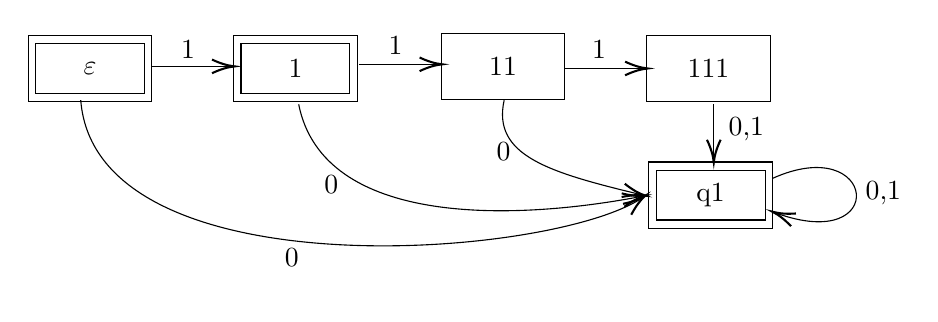
\begin{tikzpicture}[x=0.75pt,y=0.75pt,yscale=-1,xscale=1]
		%uncomment if require: \path (0,273.1999988555908); %set diagram left start at 0, and has height of 273.1999988555908
		
		%Shape: Rectangle [id:dp01033379984949967] 
		\draw   (219,70) -- (278.5,70) -- (278.5,101.91) -- (219,101.91) -- cycle ;
		%Straight Lines [id:da6875355876086366] 
		\draw    (179.5,84.91) -- (217.5,84.91) ;
		\draw [shift={(219.5,84.91)}, rotate = 180] [color={rgb, 255:red, 0; green, 0; blue, 0 }  ][line width=0.75]    (10.93,-3.29) .. controls (6.95,-1.4) and (3.31,-0.3) .. (0,0) .. controls (3.31,0.3) and (6.95,1.4) .. (10.93,3.29)   ;
		
		%Shape: Rectangle [id:dp795794424190027] 
		\draw   (319,69) -- (378.5,69) -- (378.5,100.91) -- (319,100.91) -- cycle ;
		%Straight Lines [id:da7394367190736346] 
		\draw    (279.5,83.91) -- (317.5,83.91) ;
		\draw [shift={(319.5,83.91)}, rotate = 180] [color={rgb, 255:red, 0; green, 0; blue, 0 }  ][line width=0.75]    (10.93,-3.29) .. controls (6.95,-1.4) and (3.31,-0.3) .. (0,0) .. controls (3.31,0.3) and (6.95,1.4) .. (10.93,3.29)   ;
		
		%Shape: Rectangle [id:dp16317497648194257] 
		\draw   (418,70) -- (477.5,70) -- (477.5,101.91) -- (418,101.91) -- cycle ;
		%Straight Lines [id:da5350031687411856] 
		\draw    (378.5,85.91) -- (416.5,85.91) ;
		\draw [shift={(418.5,85.91)}, rotate = 180] [color={rgb, 255:red, 0; green, 0; blue, 0 }  ][line width=0.75]    (10.93,-3.29) .. controls (6.95,-1.4) and (3.31,-0.3) .. (0,0) .. controls (3.31,0.3) and (6.95,1.4) .. (10.93,3.29)   ;
		
		%Shape: Rectangle [id:dp1578010021865861] 
		\draw   (120,70) -- (179.5,70) -- (179.5,101.91) -- (120,101.91) -- cycle ;
		%Shape: Rectangle [id:dp24537568713707536] 
		\draw   (422.5,135) -- (475,135) -- (475,158.91) -- (422.5,158.91) -- cycle ;
		%Shape: Rectangle [id:dp10047697590078752] 
		\draw   (419,131) -- (478.5,131) -- (478.5,162.91) -- (419,162.91) -- cycle ;
		%Curve Lines [id:da5630328613347559] 
		\draw    (478.5,138.91) .. controls (528.99,116.14) and (535.38,175.69) .. (480.19,155.54) ;
		\draw [shift={(478.5,154.91)}, rotate = 381.1] [color={rgb, 255:red, 0; green, 0; blue, 0 }  ][line width=0.75]    (10.93,-3.29) .. controls (6.95,-1.4) and (3.31,-0.3) .. (0,0) .. controls (3.31,0.3) and (6.95,1.4) .. (10.93,3.29)   ;
		
		%Straight Lines [id:da7208662592083559] 
		\draw    (450.3,103.2) -- (450.3,129.2) ;
		\draw [shift={(450.3,131.2)}, rotate = 270] [color={rgb, 255:red, 0; green, 0; blue, 0 }  ][line width=0.75]    (10.93,-3.29) .. controls (6.95,-1.4) and (3.31,-0.3) .. (0,0) .. controls (3.31,0.3) and (6.95,1.4) .. (10.93,3.29)   ;
		
		%Curve Lines [id:da3882070037651799] 
		\draw    (145.3,101.2) .. controls (152.53,194.46) and (372.83,177.55) .. (416.04,148.1) ;
		\draw [shift={(417.3,147.2)}, rotate = 503.13] [color={rgb, 255:red, 0; green, 0; blue, 0 }  ][line width=0.75]    (10.93,-3.29) .. controls (6.95,-1.4) and (3.31,-0.3) .. (0,0) .. controls (3.31,0.3) and (6.95,1.4) .. (10.93,3.29)   ;
		
		%Curve Lines [id:da266009885816783] 
		\draw    (250.3,103.2) .. controls (262.18,162.6) and (354.43,159.27) .. (415.46,147.56) ;
		\draw [shift={(417.3,147.2)}, rotate = 528.87] [color={rgb, 255:red, 0; green, 0; blue, 0 }  ][line width=0.75]    (10.93,-3.29) .. controls (6.95,-1.4) and (3.31,-0.3) .. (0,0) .. controls (3.31,0.3) and (6.95,1.4) .. (10.93,3.29)   ;
		
		%Curve Lines [id:da45207501780132664] 
		\draw    (349.3,101.2) .. controls (343.36,127.93) and (370.74,136.04) .. (415.93,146.87) ;
		\draw [shift={(417.3,147.2)}, rotate = 193.45] [color={rgb, 255:red, 0; green, 0; blue, 0 }  ][line width=0.75]    (10.93,-3.29) .. controls (6.95,-1.4) and (3.31,-0.3) .. (0,0) .. controls (3.31,0.3) and (6.95,1.4) .. (10.93,3.29)   ;
		
		%Shape: Rectangle [id:dp18468687089700042] 
		\draw   (222.5,74) -- (275,74) -- (275,97.91) -- (222.5,97.91) -- cycle ;
		%Shape: Rectangle [id:dp2986797080644137] 
		\draw   (123.5,74) -- (176,74) -- (176,97.91) -- (123.5,97.91) -- cycle ;
		
		% Text Node
		\draw (297,75) node  [align=left] {1};
		% Text Node
		\draw (248.75,85.95) node  [align=left] {1};
		% Text Node
		\draw (348.75,84.95) node  [align=left] {11};
		% Text Node
		\draw (395,77) node  [align=left] {1};
		% Text Node
		\draw (447.75,85.95) node  [align=left] {111};
		% Text Node
		\draw (149.75,85.95) node  [align=left] {$\varepsilon$};
		% Text Node
		\draw (197,77) node  [align=left] {1};
		% Text Node
		\draw (448.75,146.95) node  [align=left] {q1};
		% Text Node
		\draw (532,146) node  [align=left] {0,1};
		% Text Node
		\draw (466,115) node  [align=left] {0,1};
		% Text Node
		\draw (247,177) node  [align=left] {0};
		% Text Node
		\draw (266,142) node  [align=left] {0};
		% Text Node
		\draw (349,126) node  [align=left] {0};
		
		\end{tikzpicture}

	\item[(i)]
		L = $\{ \:\{ \varepsilon, q0, 1, q1\}, \{0, 1\}, \delta, \varepsilon, \{q0, 1\}\}$	\\
		$\delta = 
		\begin{array}{ c|c|c }
			 & 0 & 1\\
			\hline
			\varepsilon & q1 & 1\\
			\hline
			1 & q0 & q0\\
			\hline
			q0 & q1 & 1\\
			\hline
			q1 & q1 & q1
		\end{array}$\\

		State diagram:

		\tikzset{every picture/.style={line width=0.75pt}} %set default line width to 0.75pt        
		
		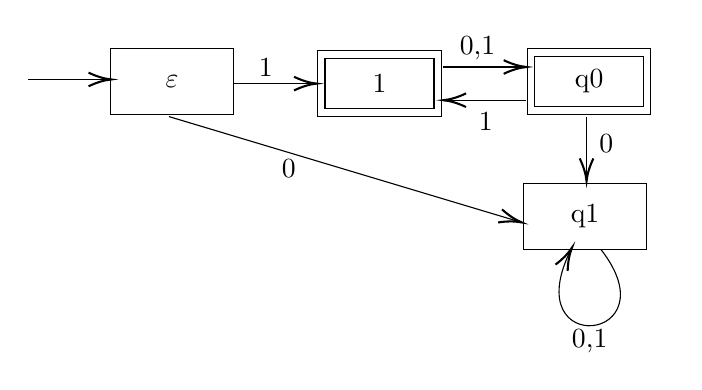
\begin{tikzpicture}[x=0.75pt,y=0.75pt,yscale=-1,xscale=1]
		%uncomment if require: \path (0,273.1999988555908); %set diagram left start at 0, and has height of 273.1999988555908
		
		%Shape: Rectangle [id:dp9162894208189922] 
		\draw   (350,58) -- (409.5,58) -- (409.5,89.91) -- (350,89.91) -- cycle ;
		%Straight Lines [id:da023853416522998883] 
		\draw    (208.5,74.91) -- (246.5,74.91) ;
		\draw [shift={(248.5,74.91)}, rotate = 180] [color={rgb, 255:red, 0; green, 0; blue, 0 }  ][line width=0.75]    (10.93,-3.29) .. controls (6.95,-1.4) and (3.31,-0.3) .. (0,0) .. controls (3.31,0.3) and (6.95,1.4) .. (10.93,3.29)   ;
		
		%Shape: Rectangle [id:dp7365525141439271] 
		\draw   (249,59) -- (308.5,59) -- (308.5,90.91) -- (249,90.91) -- cycle ;
		%Straight Lines [id:da30156492798223944] 
		\draw    (309.5,66.91) -- (347.5,66.91) ;
		\draw [shift={(349.5,66.91)}, rotate = 180] [color={rgb, 255:red, 0; green, 0; blue, 0 }  ][line width=0.75]    (10.93,-3.29) .. controls (6.95,-1.4) and (3.31,-0.3) .. (0,0) .. controls (3.31,0.3) and (6.95,1.4) .. (10.93,3.29)   ;
		
		%Straight Lines [id:da008961135571200263] 
		\draw    (311.5,82.91) -- (349.5,82.91) ;
		
		\draw [shift={(309.5,82.91)}, rotate = 0] [color={rgb, 255:red, 0; green, 0; blue, 0 }  ][line width=0.75]    (10.93,-3.29) .. controls (6.95,-1.4) and (3.31,-0.3) .. (0,0) .. controls (3.31,0.3) and (6.95,1.4) .. (10.93,3.29)   ;
		%Straight Lines [id:da9203511383513621] 
		\draw    (378.5,90.91) -- (378.5,119.91) ;
		\draw [shift={(378.5,121.91)}, rotate = 270] [color={rgb, 255:red, 0; green, 0; blue, 0 }  ][line width=0.75]    (10.93,-3.29) .. controls (6.95,-1.4) and (3.31,-0.3) .. (0,0) .. controls (3.31,0.3) and (6.95,1.4) .. (10.93,3.29)   ;
		
		%Shape: Rectangle [id:dp4796669634238937] 
		\draw   (348,123) -- (407.5,123) -- (407.5,154.91) -- (348,154.91) -- cycle ;
		%Curve Lines [id:da780108015464446] 
		\draw    (385.5,154.91) .. controls (420.15,199.46) and (345.03,207.74) .. (370.69,155.51) ;
		\draw [shift={(371.5,153.91)}, rotate = 477.41] [color={rgb, 255:red, 0; green, 0; blue, 0 }  ][line width=0.75]    (10.93,-3.29) .. controls (6.95,-1.4) and (3.31,-0.3) .. (0,0) .. controls (3.31,0.3) and (6.95,1.4) .. (10.93,3.29)   ;
		
		%Shape: Rectangle [id:dp2770795408517699] 
		\draw   (353.5,62) -- (406,62) -- (406,85.91) -- (353.5,85.91) -- cycle ;
		%Shape: Rectangle [id:dp1312183925135515] 
		\draw   (252.5,63) -- (305,63) -- (305,86.91) -- (252.5,86.91) -- cycle ;
		%Shape: Rectangle [id:dp4323266921750759] 
		\draw   (149,58) -- (208.5,58) -- (208.5,89.91) -- (149,89.91) -- cycle ;
		%Straight Lines [id:da19354187415046997] 
		\draw    (109.5,72.91) -- (147.5,72.91) ;
		\draw [shift={(149.5,72.91)}, rotate = 180] [color={rgb, 255:red, 0; green, 0; blue, 0 }  ][line width=0.75]    (10.93,-3.29) .. controls (6.95,-1.4) and (3.31,-0.3) .. (0,0) .. controls (3.31,0.3) and (6.95,1.4) .. (10.93,3.29)   ;
		
		%Straight Lines [id:da9784742530855985] 
		\draw    (177.3,90.8) -- (345.38,141.23) ;
		\draw [shift={(347.3,141.8)}, rotate = 196.7] [color={rgb, 255:red, 0; green, 0; blue, 0 }  ][line width=0.75]    (10.93,-3.29) .. controls (6.95,-1.4) and (3.31,-0.3) .. (0,0) .. controls (3.31,0.3) and (6.95,1.4) .. (10.93,3.29)   ;
		
		% Text Node
		\draw (379.75,73.95) node  [align=left] {q0};
		% Text Node
		\draw (326,58) node  [align=left] {0,1};
		% Text Node
		\draw (278.75,74.95) node  [align=left] {1};
		% Text Node
		\draw (330,93) node  [align=left] {1};
		% Text Node
		\draw (388,104) node  [align=left] {0};
		% Text Node
		\draw (380,199) node  [align=left] {0,1};
		% Text Node
		\draw (377.75,138.95) node  [align=left] {q1};
		% Text Node
		\draw (178.75,73.95) node  [align=left] {$\varepsilon$};
		% Text Node
		\draw (224,67) node  [align=left] {1};
		% Text Node
		\draw (235,116) node  [align=left] {0};
		
		\end{tikzpicture}

	\item[(j)]
		L = $\{ \:\{ \varepsilon, 0, 00, 1, 01, 001, 11\}, \{0, 1\}, \delta, \varepsilon, \{00, 001\}\}$	\\
		$\delta = 
		\begin{array}{ c|c|c }
			 & 0 & 1\\
			\hline
			\varepsilon & 0 & 1\\
			\hline
			0 & 00 & 01\\
			\hline
			00 & 00 & 001\\
			\hline
			1 & 01 & 11\\
			\hline
			01 & 001 & 11\\
			\hline
			001 & 001 & 11\\
			\hline
			11 & 11 & 11
		\end{array}$\\

		State diagram:

		\tikzset{every picture/.style={line width=0.75pt}} %set default line width to 0.75pt        
		
		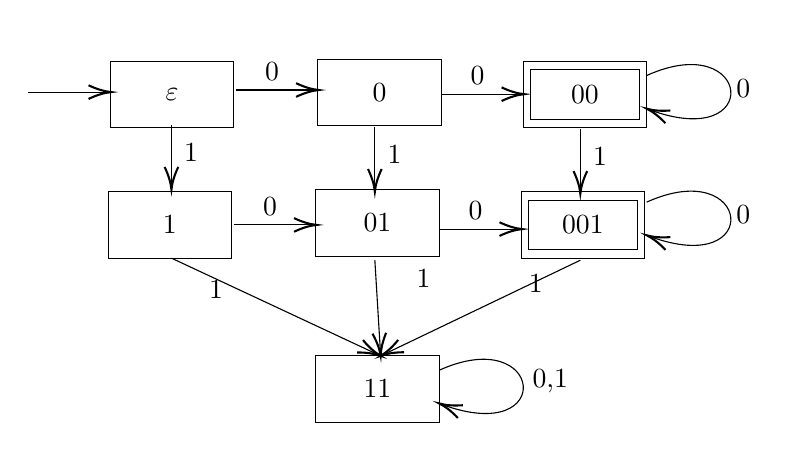
\begin{tikzpicture}[x=0.75pt,y=0.75pt,yscale=-1,xscale=1]
		%uncomment if require: \path (0,273.1999988555908); %set diagram left start at 0, and has height of 273.1999988555908
		
		%Shape: Rectangle [id:dp233631449647548] 
		\draw   (222,59) -- (281.5,59) -- (281.5,90.91) -- (222,90.91) -- cycle ;
		%Straight Lines [id:da43015843737015946] 
		\draw    (182.5,73.91) -- (220.5,73.91) ;
		\draw [shift={(222.5,73.91)}, rotate = 180] [color={rgb, 255:red, 0; green, 0; blue, 0 }  ][line width=0.75]    (10.93,-3.29) .. controls (6.95,-1.4) and (3.31,-0.3) .. (0,0) .. controls (3.31,0.3) and (6.95,1.4) .. (10.93,3.29)   ;
		
		%Straight Lines [id:da23445778052858945] 
		\draw    (251.5,89.91) -- (251.5,118.91) ;
		\draw [shift={(251.5,120.91)}, rotate = 270] [color={rgb, 255:red, 0; green, 0; blue, 0 }  ][line width=0.75]    (10.93,-3.29) .. controls (6.95,-1.4) and (3.31,-0.3) .. (0,0) .. controls (3.31,0.3) and (6.95,1.4) .. (10.93,3.29)   ;
		
		%Shape: Rectangle [id:dp03569261507208221] 
		\draw   (322,58) -- (381.5,58) -- (381.5,89.91) -- (322,89.91) -- cycle ;
		%Straight Lines [id:da7075906395966309] 
		\draw    (282.5,72.91) -- (320.5,72.91) ;
		\draw [shift={(322.5,72.91)}, rotate = 180] [color={rgb, 255:red, 0; green, 0; blue, 0 }  ][line width=0.75]    (10.93,-3.29) .. controls (6.95,-1.4) and (3.31,-0.3) .. (0,0) .. controls (3.31,0.3) and (6.95,1.4) .. (10.93,3.29)   ;
		
		%Shape: Rectangle [id:dp1927664938247382] 
		\draw   (221,122) -- (280.5,122) -- (280.5,153.91) -- (221,153.91) -- cycle ;
		%Shape: Rectangle [id:dp4826802014961502] 
		\draw   (321,121) -- (380.5,121) -- (380.5,152.91) -- (321,152.91) -- cycle ;
		%Curve Lines [id:da12097553359067481] 
		\draw    (480.5,65.91) .. controls (530.99,43.14) and (537.38,102.69) .. (482.19,82.54) ;
		\draw [shift={(480.5,81.91)}, rotate = 381.1] [color={rgb, 255:red, 0; green, 0; blue, 0 }  ][line width=0.75]    (10.93,-3.29) .. controls (6.95,-1.4) and (3.31,-0.3) .. (0,0) .. controls (3.31,0.3) and (6.95,1.4) .. (10.93,3.29)   ;
		
		%Curve Lines [id:da39342689601335135] 
		\draw    (480.5,126.91) .. controls (530.99,104.14) and (537.38,163.69) .. (482.19,143.54) ;
		\draw [shift={(480.5,142.91)}, rotate = 381.1] [color={rgb, 255:red, 0; green, 0; blue, 0 }  ][line width=0.75]    (10.93,-3.29) .. controls (6.95,-1.4) and (3.31,-0.3) .. (0,0) .. controls (3.31,0.3) and (6.95,1.4) .. (10.93,3.29)   ;
		
		%Straight Lines [id:da4816225771869793] 
		\draw    (281.5,137.91) -- (319.5,137.91) ;
		\draw [shift={(321.5,137.91)}, rotate = 180] [color={rgb, 255:red, 0; green, 0; blue, 0 }  ][line width=0.75]    (10.93,-3.29) .. controls (6.95,-1.4) and (3.31,-0.3) .. (0,0) .. controls (3.31,0.3) and (6.95,1.4) .. (10.93,3.29)   ;
		
		%Straight Lines [id:da09593236793301618] 
		\draw    (349.5,90.91) -- (349.5,119.91) ;
		\draw [shift={(349.5,121.91)}, rotate = 270] [color={rgb, 255:red, 0; green, 0; blue, 0 }  ][line width=0.75]    (10.93,-3.29) .. controls (6.95,-1.4) and (3.31,-0.3) .. (0,0) .. controls (3.31,0.3) and (6.95,1.4) .. (10.93,3.29)   ;
		
		%Shape: Rectangle [id:dp15985928870288157] 
		\draw   (421,59) -- (480.5,59) -- (480.5,90.91) -- (421,90.91) -- cycle ;
		%Straight Lines [id:da9774639656759714] 
		\draw    (381.5,74.91) -- (419.5,74.91) ;
		\draw [shift={(421.5,74.91)}, rotate = 180] [color={rgb, 255:red, 0; green, 0; blue, 0 }  ][line width=0.75]    (10.93,-3.29) .. controls (6.95,-1.4) and (3.31,-0.3) .. (0,0) .. controls (3.31,0.3) and (6.95,1.4) .. (10.93,3.29)   ;
		
		%Shape: Rectangle [id:dp8255534179053012] 
		\draw   (420,122) -- (479.5,122) -- (479.5,153.91) -- (420,153.91) -- cycle ;
		%Straight Lines [id:da27063923149560964] 
		\draw    (380.5,139.91) -- (418.5,139.91) ;
		\draw [shift={(420.5,139.91)}, rotate = 180] [color={rgb, 255:red, 0; green, 0; blue, 0 }  ][line width=0.75]    (10.93,-3.29) .. controls (6.95,-1.4) and (3.31,-0.3) .. (0,0) .. controls (3.31,0.3) and (6.95,1.4) .. (10.93,3.29)   ;
		
		%Straight Lines [id:da43477093862482397] 
		\draw    (448.5,91.91) -- (448.5,120.91) ;
		\draw [shift={(448.5,122.91)}, rotate = 270] [color={rgb, 255:red, 0; green, 0; blue, 0 }  ][line width=0.75]    (10.93,-3.29) .. controls (6.95,-1.4) and (3.31,-0.3) .. (0,0) .. controls (3.31,0.3) and (6.95,1.4) .. (10.93,3.29)   ;
		
		%Straight Lines [id:da5217215937856232] 
		\draw    (251.5,153.91) -- (350.49,200.15) ;
		\draw [shift={(352.3,201)}, rotate = 205.04] [color={rgb, 255:red, 0; green, 0; blue, 0 }  ][line width=0.75]    (10.93,-3.29) .. controls (6.95,-1.4) and (3.31,-0.3) .. (0,0) .. controls (3.31,0.3) and (6.95,1.4) .. (10.93,3.29)   ;
		
		%Curve Lines [id:da23463425085479317] 
		\draw    (380.5,207.91) .. controls (430.99,185.14) and (437.38,244.69) .. (382.19,224.54) ;
		\draw [shift={(380.5,223.91)}, rotate = 381.1] [color={rgb, 255:red, 0; green, 0; blue, 0 }  ][line width=0.75]    (10.93,-3.29) .. controls (6.95,-1.4) and (3.31,-0.3) .. (0,0) .. controls (3.31,0.3) and (6.95,1.4) .. (10.93,3.29)   ;
		
		%Straight Lines [id:da738047602323793] 
		\draw    (349.5,154.91) -- (352.18,199) ;
		\draw [shift={(352.3,201)}, rotate = 266.52] [color={rgb, 255:red, 0; green, 0; blue, 0 }  ][line width=0.75]    (10.93,-3.29) .. controls (6.95,-1.4) and (3.31,-0.3) .. (0,0) .. controls (3.31,0.3) and (6.95,1.4) .. (10.93,3.29)   ;
		
		%Straight Lines [id:da4109932081024965] 
		\draw    (448.5,154.91) -- (354.1,200.14) ;
		\draw [shift={(352.3,201)}, rotate = 334.4] [color={rgb, 255:red, 0; green, 0; blue, 0 }  ][line width=0.75]    (10.93,-3.29) .. controls (6.95,-1.4) and (3.31,-0.3) .. (0,0) .. controls (3.31,0.3) and (6.95,1.4) .. (10.93,3.29)   ;
		
		%Shape: Rectangle [id:dp5869349555712065] 
		\draw   (321,201) -- (380.5,201) -- (380.5,232.91) -- (321,232.91) -- cycle ;
		%Shape: Rectangle [id:dp38040662411927717] 
		\draw   (424.5,63) -- (477,63) -- (477,86.91) -- (424.5,86.91) -- cycle ;
		%Shape: Rectangle [id:dp6928570845668118] 
		\draw   (423.5,126) -- (476,126) -- (476,149.91) -- (423.5,149.91) -- cycle ;
		
		% Text Node
		\draw (300,64) node  [align=left] {0};
		% Text Node
		\draw (299,129) node  [align=left] {0};
		% Text Node
		\draw (527,72) node  [align=left] {0};
		% Text Node
		\draw (527,133) node  [align=left] {0};
		% Text Node
		\draw (261,103) node  [align=left] {1};
		% Text Node
		\draw (359,104) node  [align=left] {1};
		% Text Node
		\draw (251.75,74.95) node  [align=left] {$\varepsilon$};
		% Text Node
		\draw (351.75,73.95) node  [align=left] {0};
		% Text Node
		\draw (250.75,137.95) node  [align=left] {1};
		% Text Node
		\draw (350.75,136.95) node  [align=left] {01};
		% Text Node
		\draw (399,66) node  [align=left] {0};
		% Text Node
		\draw (398,131) node  [align=left] {0};
		% Text Node
		\draw (458,105) node  [align=left] {1};
		% Text Node
		\draw (450.75,74.95) node  [align=left] {00};
		% Text Node
		\draw (449.75,137.95) node  [align=left] {001};
		% Text Node
		\draw (273,169) node  [align=left] {1};
		% Text Node
		\draw (373,164) node  [align=left] {1};
		% Text Node
		\draw (427,166) node  [align=left] {1};
		% Text Node
		\draw (350.75,216.95) node  [align=left] {11};
		% Text Node
		\draw (434,213) node  [align=left] {0,1};
		
		\end{tikzpicture}

	\item[(k)]	
		L = $\{ \:\{ \varepsilon, 0, q1\}, \{0, 1\}, \delta, \varepsilon, \{ \varepsilon, 0\}\}$	\\
		$\delta = 
		\begin{array}{ c|c|c }
			 & 0 & 1\\
			\hline
			\varepsilon & 0 & q1\\
			\hline
			0 & q1 & q1\\
			\hline
			q1 & q1 & q1
		\end{array}$\\

		State diagram:

		\tikzset{every picture/.style={line width=0.75pt}} %set default line width to 0.75pt        
		
		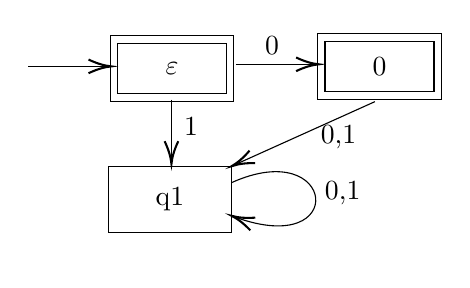
\begin{tikzpicture}[x=0.75pt,y=0.75pt,yscale=-1,xscale=1]
		%uncomment if require: \path (0,273.1999988555908); %set diagram left start at 0, and has height of 273.1999988555908
		
		%Shape: Rectangle [id:dp19405751181386366] 
		\draw   (222,59) -- (281.5,59) -- (281.5,90.91) -- (222,90.91) -- cycle ;
		%Straight Lines [id:da9370717933278756] 
		\draw    (182.5,73.91) -- (220.5,73.91) ;
		\draw [shift={(222.5,73.91)}, rotate = 180] [color={rgb, 255:red, 0; green, 0; blue, 0 }  ][line width=0.75]    (10.93,-3.29) .. controls (6.95,-1.4) and (3.31,-0.3) .. (0,0) .. controls (3.31,0.3) and (6.95,1.4) .. (10.93,3.29)   ;
		
		%Straight Lines [id:da39549705173893734] 
		\draw    (251.5,89.91) -- (251.5,118.91) ;
		\draw [shift={(251.5,120.91)}, rotate = 270] [color={rgb, 255:red, 0; green, 0; blue, 0 }  ][line width=0.75]    (10.93,-3.29) .. controls (6.95,-1.4) and (3.31,-0.3) .. (0,0) .. controls (3.31,0.3) and (6.95,1.4) .. (10.93,3.29)   ;
		
		%Shape: Rectangle [id:dp003907149593821213] 
		\draw   (322,58) -- (381.5,58) -- (381.5,89.91) -- (322,89.91) -- cycle ;
		%Straight Lines [id:da6455238766475018] 
		\draw    (282.5,72.91) -- (320.5,72.91) ;
		\draw [shift={(322.5,72.91)}, rotate = 180] [color={rgb, 255:red, 0; green, 0; blue, 0 }  ][line width=0.75]    (10.93,-3.29) .. controls (6.95,-1.4) and (3.31,-0.3) .. (0,0) .. controls (3.31,0.3) and (6.95,1.4) .. (10.93,3.29)   ;
		
		%Shape: Rectangle [id:dp1314203170578847] 
		\draw   (221,122) -- (280.5,122) -- (280.5,153.91) -- (221,153.91) -- cycle ;
		%Straight Lines [id:da9201118400950614] 
		\draw    (349.5,90.91) -- (282.32,121.18) ;
		\draw [shift={(280.5,122)}, rotate = 335.74] [color={rgb, 255:red, 0; green, 0; blue, 0 }  ][line width=0.75]    (10.93,-3.29) .. controls (6.95,-1.4) and (3.31,-0.3) .. (0,0) .. controls (3.31,0.3) and (6.95,1.4) .. (10.93,3.29)   ;
		
		%Curve Lines [id:da320795518307333] 
		\draw    (280.5,129.91) .. controls (330.99,107.14) and (337.38,166.69) .. (282.19,146.54) ;
		\draw [shift={(280.5,145.91)}, rotate = 381.1] [color={rgb, 255:red, 0; green, 0; blue, 0 }  ][line width=0.75]    (10.93,-3.29) .. controls (6.95,-1.4) and (3.31,-0.3) .. (0,0) .. controls (3.31,0.3) and (6.95,1.4) .. (10.93,3.29)   ;
		
		%Shape: Rectangle [id:dp08456474897349975] 
		\draw   (225.5,63) -- (278,63) -- (278,86.91) -- (225.5,86.91) -- cycle ;
		%Shape: Rectangle [id:dp15464561789405096] 
		\draw   (325.5,62) -- (378,62) -- (378,85.91) -- (325.5,85.91) -- cycle ;
		
		% Text Node
		\draw (300,64) node  [align=left] {0};
		% Text Node
		\draw (261,103) node  [align=left] {1};
		% Text Node
		\draw (332,108) node  [align=left] {0,1};
		% Text Node
		\draw (251.75,74.95) node  [align=left] {$\varepsilon$};
		% Text Node
		\draw (351.75,73.95) node  [align=left] {0};
		% Text Node
		\draw (250.75,137.95) node  [align=left] {q1};
		% Text Node
		\draw (334,135) node  [align=left] {0,1};
		
		\end{tikzpicture}

	\item[(l)]	
		L = $\{ \:\{ \varepsilon, 1, 11, 111, 0, 01, 011, 0111\}, \{0, 1\}, \delta, \varepsilon, \{ \varepsilon, 1, 11, 111, 011\}\}$	\\
		$\delta = 
		\begin{array}{ c|c|c }
			 & 0 & 1\\
			\hline
			\varepsilon & 0 & 1\\
			\hline
			1 & 01 & 11\\
			\hline
			11 & 011 & 111\\
			\hline
			111 & 0111 & 111\\
			\hline
			0 & \varepsilon & 01\\
			\hline
			01 & 1 & 011\\
			\hline
			011 & 11 & 0111\\
			\hline
			0111 & 111 & 0111
		\end{array}$\\

		State diagram:

		\tikzset{every picture/.style={line width=0.75pt}} %set default line width to 0.75pt        
		
		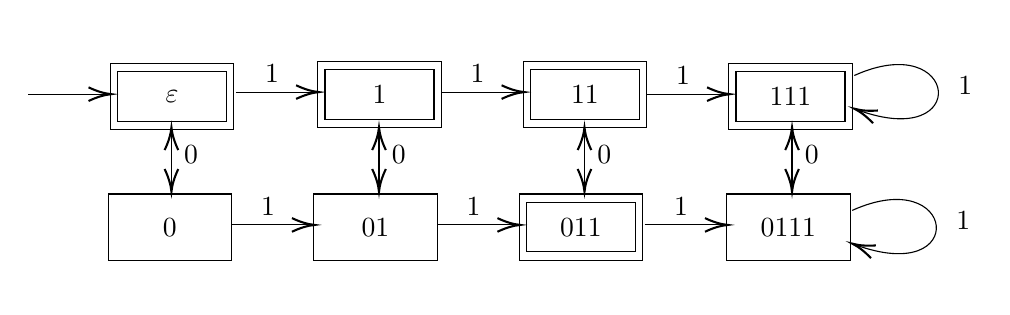
\begin{tikzpicture}[x=0.75pt,y=0.75pt,yscale=-1,xscale=1]
		%uncomment if require: \path (0,273.1999988555908); %set diagram left start at 0, and has height of 273.1999988555908
		
		%Shape: Rectangle [id:dp3482758894622664] 
		\draw   (222,59) -- (281.5,59) -- (281.5,90.91) -- (222,90.91) -- cycle ;
		%Straight Lines [id:da46626186871468334] 
		\draw    (182.5,73.91) -- (220.5,73.91) ;
		\draw [shift={(222.5,73.91)}, rotate = 180] [color={rgb, 255:red, 0; green, 0; blue, 0 }  ][line width=0.75]    (10.93,-3.29) .. controls (6.95,-1.4) and (3.31,-0.3) .. (0,0) .. controls (3.31,0.3) and (6.95,1.4) .. (10.93,3.29)   ;
		
		%Straight Lines [id:da9567690913585047] 
		\draw    (251.5,91.91) -- (251.5,118.91) ;
		\draw [shift={(251.5,120.91)}, rotate = 270] [color={rgb, 255:red, 0; green, 0; blue, 0 }  ][line width=0.75]    (10.93,-3.29) .. controls (6.95,-1.4) and (3.31,-0.3) .. (0,0) .. controls (3.31,0.3) and (6.95,1.4) .. (10.93,3.29)   ;
		\draw [shift={(251.5,89.91)}, rotate = 90] [color={rgb, 255:red, 0; green, 0; blue, 0 }  ][line width=0.75]    (10.93,-3.29) .. controls (6.95,-1.4) and (3.31,-0.3) .. (0,0) .. controls (3.31,0.3) and (6.95,1.4) .. (10.93,3.29)   ;
		%Shape: Rectangle [id:dp6028466345274555] 
		\draw   (322,58) -- (381.5,58) -- (381.5,89.91) -- (322,89.91) -- cycle ;
		%Straight Lines [id:da6406222345633479] 
		\draw    (282.5,72.91) -- (320.5,72.91) ;
		\draw [shift={(322.5,72.91)}, rotate = 180] [color={rgb, 255:red, 0; green, 0; blue, 0 }  ][line width=0.75]    (10.93,-3.29) .. controls (6.95,-1.4) and (3.31,-0.3) .. (0,0) .. controls (3.31,0.3) and (6.95,1.4) .. (10.93,3.29)   ;
		
		%Shape: Rectangle [id:dp5434778568064202] 
		\draw   (221,122) -- (280.5,122) -- (280.5,153.91) -- (221,153.91) -- cycle ;
		%Shape: Rectangle [id:dp3106379990265429] 
		\draw   (421,58) -- (480.5,58) -- (480.5,89.91) -- (421,89.91) -- cycle ;
		%Straight Lines [id:da873075140241993] 
		\draw    (381.5,72.91) -- (419.5,72.91) ;
		\draw [shift={(421.5,72.91)}, rotate = 180] [color={rgb, 255:red, 0; green, 0; blue, 0 }  ][line width=0.75]    (10.93,-3.29) .. controls (6.95,-1.4) and (3.31,-0.3) .. (0,0) .. controls (3.31,0.3) and (6.95,1.4) .. (10.93,3.29)   ;
		
		%Shape: Rectangle [id:dp12759586455369498] 
		\draw   (520,59) -- (579.5,59) -- (579.5,90.91) -- (520,90.91) -- cycle ;
		%Straight Lines [id:da0328314263826508] 
		\draw    (480.5,73.91) -- (518.5,73.91) ;
		\draw [shift={(520.5,73.91)}, rotate = 180] [color={rgb, 255:red, 0; green, 0; blue, 0 }  ][line width=0.75]    (10.93,-3.29) .. controls (6.95,-1.4) and (3.31,-0.3) .. (0,0) .. controls (3.31,0.3) and (6.95,1.4) .. (10.93,3.29)   ;
		
		%Shape: Rectangle [id:dp27560489543908906] 
		\draw   (320,122) -- (379.5,122) -- (379.5,153.91) -- (320,153.91) -- cycle ;
		%Straight Lines [id:da6801205728951314] 
		\draw    (280.5,136.91) -- (318.5,136.91) ;
		\draw [shift={(320.5,136.91)}, rotate = 180] [color={rgb, 255:red, 0; green, 0; blue, 0 }  ][line width=0.75]    (10.93,-3.29) .. controls (6.95,-1.4) and (3.31,-0.3) .. (0,0) .. controls (3.31,0.3) and (6.95,1.4) .. (10.93,3.29)   ;
		
		%Straight Lines [id:da4041443541138845] 
		\draw    (351.5,91.91) -- (351.5,118.91) ;
		\draw [shift={(351.5,120.91)}, rotate = 270] [color={rgb, 255:red, 0; green, 0; blue, 0 }  ][line width=0.75]    (10.93,-3.29) .. controls (6.95,-1.4) and (3.31,-0.3) .. (0,0) .. controls (3.31,0.3) and (6.95,1.4) .. (10.93,3.29)   ;
		\draw [shift={(351.5,89.91)}, rotate = 90] [color={rgb, 255:red, 0; green, 0; blue, 0 }  ][line width=0.75]    (10.93,-3.29) .. controls (6.95,-1.4) and (3.31,-0.3) .. (0,0) .. controls (3.31,0.3) and (6.95,1.4) .. (10.93,3.29)   ;
		%Shape: Rectangle [id:dp27047592976291956] 
		\draw   (419,122) -- (478.5,122) -- (478.5,153.91) -- (419,153.91) -- cycle ;
		%Straight Lines [id:da8342969379728149] 
		\draw    (379.5,136.91) -- (417.5,136.91) ;
		\draw [shift={(419.5,136.91)}, rotate = 180] [color={rgb, 255:red, 0; green, 0; blue, 0 }  ][line width=0.75]    (10.93,-3.29) .. controls (6.95,-1.4) and (3.31,-0.3) .. (0,0) .. controls (3.31,0.3) and (6.95,1.4) .. (10.93,3.29)   ;
		
		%Straight Lines [id:da426076887980382] 
		\draw    (450.5,91.91) -- (450.5,118.91) ;
		\draw [shift={(450.5,120.91)}, rotate = 270] [color={rgb, 255:red, 0; green, 0; blue, 0 }  ][line width=0.75]    (10.93,-3.29) .. controls (6.95,-1.4) and (3.31,-0.3) .. (0,0) .. controls (3.31,0.3) and (6.95,1.4) .. (10.93,3.29)   ;
		\draw [shift={(450.5,89.91)}, rotate = 90] [color={rgb, 255:red, 0; green, 0; blue, 0 }  ][line width=0.75]    (10.93,-3.29) .. controls (6.95,-1.4) and (3.31,-0.3) .. (0,0) .. controls (3.31,0.3) and (6.95,1.4) .. (10.93,3.29)   ;
		%Shape: Rectangle [id:dp2488674554965602] 
		\draw   (519,122) -- (578.5,122) -- (578.5,153.91) -- (519,153.91) -- cycle ;
		%Straight Lines [id:da8357711468482352] 
		\draw    (479.5,136.91) -- (517.5,136.91) ;
		\draw [shift={(519.5,136.91)}, rotate = 180] [color={rgb, 255:red, 0; green, 0; blue, 0 }  ][line width=0.75]    (10.93,-3.29) .. controls (6.95,-1.4) and (3.31,-0.3) .. (0,0) .. controls (3.31,0.3) and (6.95,1.4) .. (10.93,3.29)   ;
		
		%Straight Lines [id:da7486778897763438] 
		\draw    (550.5,91.91) -- (550.5,118.91) ;
		\draw [shift={(550.5,120.91)}, rotate = 270] [color={rgb, 255:red, 0; green, 0; blue, 0 }  ][line width=0.75]    (10.93,-3.29) .. controls (6.95,-1.4) and (3.31,-0.3) .. (0,0) .. controls (3.31,0.3) and (6.95,1.4) .. (10.93,3.29)   ;
		\draw [shift={(550.5,89.91)}, rotate = 90] [color={rgb, 255:red, 0; green, 0; blue, 0 }  ][line width=0.75]    (10.93,-3.29) .. controls (6.95,-1.4) and (3.31,-0.3) .. (0,0) .. controls (3.31,0.3) and (6.95,1.4) .. (10.93,3.29)   ;
		%Curve Lines [id:da5413921926026104] 
		\draw    (580.5,64.91) .. controls (630.99,42.14) and (637.38,101.69) .. (582.19,81.54) ;
		\draw [shift={(580.5,80.91)}, rotate = 381.1] [color={rgb, 255:red, 0; green, 0; blue, 0 }  ][line width=0.75]    (10.93,-3.29) .. controls (6.95,-1.4) and (3.31,-0.3) .. (0,0) .. controls (3.31,0.3) and (6.95,1.4) .. (10.93,3.29)   ;
		
		%Curve Lines [id:da4295105155425416] 
		\draw    (579.5,129.91) .. controls (629.99,107.14) and (636.38,166.69) .. (581.19,146.54) ;
		\draw [shift={(579.5,145.91)}, rotate = 381.1] [color={rgb, 255:red, 0; green, 0; blue, 0 }  ][line width=0.75]    (10.93,-3.29) .. controls (6.95,-1.4) and (3.31,-0.3) .. (0,0) .. controls (3.31,0.3) and (6.95,1.4) .. (10.93,3.29)   ;
		
		%Shape: Rectangle [id:dp2687046097806529] 
		\draw   (424.5,62) -- (477,62) -- (477,85.91) -- (424.5,85.91) -- cycle ;
		%Shape: Rectangle [id:dp051563041549212096] 
		\draw   (523.5,63) -- (576,63) -- (576,86.91) -- (523.5,86.91) -- cycle ;
		%Shape: Rectangle [id:dp875949154953209] 
		\draw   (325.5,62) -- (378,62) -- (378,85.91) -- (325.5,85.91) -- cycle ;
		%Shape: Rectangle [id:dp08431890689063959] 
		\draw   (225.5,63) -- (278,63) -- (278,86.91) -- (225.5,86.91) -- cycle ;
		%Shape: Rectangle [id:dp25390038621108646] 
		\draw   (422.5,126) -- (475,126) -- (475,149.91) -- (422.5,149.91) -- cycle ;
		
		% Text Node
		\draw (300,64) node  [align=left] {1};
		% Text Node
		\draw (261,103) node  [align=left] {0};
		% Text Node
		\draw (251.75,74.95) node  [align=left] {$\varepsilon$};
		% Text Node
		\draw (351.75,73.95) node  [align=left] {1};
		% Text Node
		\draw (250.75,137.95) node  [align=left] {0};
		% Text Node
		\draw (399,64) node  [align=left] {1};
		% Text Node
		\draw (450.75,73.95) node  [align=left] {11};
		% Text Node
		\draw (498,65) node  [align=left] {1};
		% Text Node
		\draw (549.75,74.95) node  [align=left] {111};
		% Text Node
		\draw (298,128) node  [align=left] {1};
		% Text Node
		\draw (349.75,137.95) node  [align=left] {01};
		% Text Node
		\draw (361,103) node  [align=left] {0};
		% Text Node
		\draw (397,128) node  [align=left] {1};
		% Text Node
		\draw (448.75,137.95) node  [align=left] {011};
		% Text Node
		\draw (460,103) node  [align=left] {0};
		% Text Node
		\draw (497,128) node  [align=left] {1};
		% Text Node
		\draw (548.75,137.95) node  [align=left] {0111};
		% Text Node
		\draw (560,103) node  [align=left] {0};
		% Text Node
		\draw (634,70) node  [align=left] {1};
		% Text Node
		\draw (633,135) node  [align=left] {1};
		
		\end{tikzpicture}

	\item[(m)]
		L = $\{ \:\{ \varepsilon, q0\}, \{0, 1\}, \delta, \varepsilon, \varepsilon\}$	\\
		$\delta = 
		\begin{array}{ c|c|c }
			 & 0 & 1\\
			\hline
			\varepsilon & q0 & q0\\
			\hline
			q0 & q0 & q0
		\end{array}$\\

		State diagram:

		\tikzset{every picture/.style={line width=0.75pt}} %set default line width to 0.75pt        
		
		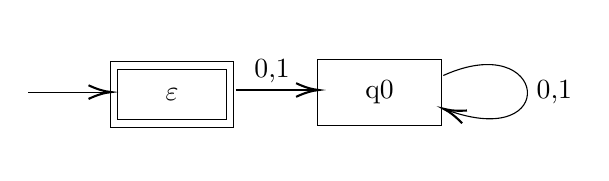
\begin{tikzpicture}[x=0.75pt,y=0.75pt,yscale=-1,xscale=1]
		%uncomment if require: \path (0,273.1999988555908); %set diagram left start at 0, and has height of 273.1999988555908
		
		%Shape: Rectangle [id:dp31897217448761017] 
		\draw   (222,59) -- (281.5,59) -- (281.5,90.91) -- (222,90.91) -- cycle ;
		%Straight Lines [id:da8147559440316081] 
		\draw    (182.5,73.91) -- (220.5,73.91) ;
		\draw [shift={(222.5,73.91)}, rotate = 180] [color={rgb, 255:red, 0; green, 0; blue, 0 }  ][line width=0.75]    (10.93,-3.29) .. controls (6.95,-1.4) and (3.31,-0.3) .. (0,0) .. controls (3.31,0.3) and (6.95,1.4) .. (10.93,3.29)   ;
		
		%Shape: Rectangle [id:dp8089717361522266] 
		\draw   (322,58) -- (381.5,58) -- (381.5,89.91) -- (322,89.91) -- cycle ;
		%Straight Lines [id:da5602162596428852] 
		\draw    (282.5,72.91) -- (320.5,72.91) ;
		\draw [shift={(322.5,72.91)}, rotate = 180] [color={rgb, 255:red, 0; green, 0; blue, 0 }  ][line width=0.75]    (10.93,-3.29) .. controls (6.95,-1.4) and (3.31,-0.3) .. (0,0) .. controls (3.31,0.3) and (6.95,1.4) .. (10.93,3.29)   ;
		
		%Curve Lines [id:da24952889551831747] 
		\draw    (382.5,65.91) .. controls (432.99,43.14) and (439.38,102.69) .. (384.19,82.54) ;
		\draw [shift={(382.5,81.91)}, rotate = 381.1] [color={rgb, 255:red, 0; green, 0; blue, 0 }  ][line width=0.75]    (10.93,-3.29) .. controls (6.95,-1.4) and (3.31,-0.3) .. (0,0) .. controls (3.31,0.3) and (6.95,1.4) .. (10.93,3.29)   ;
		
		%Shape: Rectangle [id:dp5956876750840363] 
		\draw   (225.5,63) -- (278,63) -- (278,86.91) -- (225.5,86.91) -- cycle ;
		
		% Text Node
		\draw (300,64) node  [align=left] {0,1};
		% Text Node
		\draw (251.75,74.95) node  [align=left] {$\varepsilon$};
		% Text Node
		\draw (351.75,73.95) node  [align=left] {q0};
		% Text Node
		\draw (436,74) node  [align=left] {0,1};
		
		\end{tikzpicture}

	\item[(n)]
		L = $\{ \:\{ \varepsilon, q0\}, \{0, 1\}, \delta, \varepsilon, q0\}$	\\
		$\delta = 
		\begin{array}{ c|c|c }
			 & 0 & 1\\
			\hline
			\varepsilon & q0 & q0\\
			\hline
			q0 & q0 & q0
		\end{array}$\\

		State diagram:

		\tikzset{every picture/.style={line width=0.75pt}} %set default line width to 0.75pt        
		
		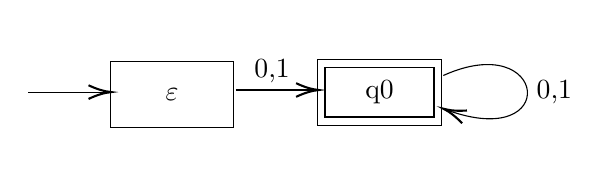
\begin{tikzpicture}[x=0.75pt,y=0.75pt,yscale=-1,xscale=1]
		%uncomment if require: \path (0,155.39999389648438); %set diagram left start at 0, and has height of 155.39999389648438
		
		%Shape: Rectangle [id:dp11849840807310041] 
		\draw   (222,59) -- (281.5,59) -- (281.5,90.91) -- (222,90.91) -- cycle ;
		%Straight Lines [id:da7879337451513004] 
		\draw    (182.5,73.91) -- (220.5,73.91) ;
		\draw [shift={(222.5,73.91)}, rotate = 180] [color={rgb, 255:red, 0; green, 0; blue, 0 }  ][line width=0.75]    (10.93,-3.29) .. controls (6.95,-1.4) and (3.31,-0.3) .. (0,0) .. controls (3.31,0.3) and (6.95,1.4) .. (10.93,3.29)   ;
		
		%Shape: Rectangle [id:dp10637030603642184] 
		\draw   (322,58) -- (381.5,58) -- (381.5,89.91) -- (322,89.91) -- cycle ;
		%Straight Lines [id:da5443791569288463] 
		\draw    (282.5,72.91) -- (320.5,72.91) ;
		\draw [shift={(322.5,72.91)}, rotate = 180] [color={rgb, 255:red, 0; green, 0; blue, 0 }  ][line width=0.75]    (10.93,-3.29) .. controls (6.95,-1.4) and (3.31,-0.3) .. (0,0) .. controls (3.31,0.3) and (6.95,1.4) .. (10.93,3.29)   ;
		
		%Curve Lines [id:da1439813025004235] 
		\draw    (382.5,65.91) .. controls (432.99,43.14) and (439.38,102.69) .. (384.19,82.54) ;
		\draw [shift={(382.5,81.91)}, rotate = 381.1] [color={rgb, 255:red, 0; green, 0; blue, 0 }  ][line width=0.75]    (10.93,-3.29) .. controls (6.95,-1.4) and (3.31,-0.3) .. (0,0) .. controls (3.31,0.3) and (6.95,1.4) .. (10.93,3.29)   ;
		
		%Shape: Rectangle [id:dp7391188231725336] 
		\draw   (325.5,62) -- (378,62) -- (378,85.91) -- (325.5,85.91) -- cycle ;
		
		% Text Node
		\draw (300,64) node  [align=left] {0,1};
		% Text Node
		\draw (251.75,74.95) node  [align=left] {$\varepsilon$};
		% Text Node
		\draw (351.75,73.95) node  [align=left] {q0};
		% Text Node
		\draw (436,74) node  [align=left] {0,1};
		
		\end{tikzpicture}

\end{enumerate}

\begin{problem}{1.7}
\end{problem}
\begin{enumerate}
	\item[(b)]	~

		\tikzset{every picture/.style={line width=0.75pt}} %set default line width to 0.75pt        
		
		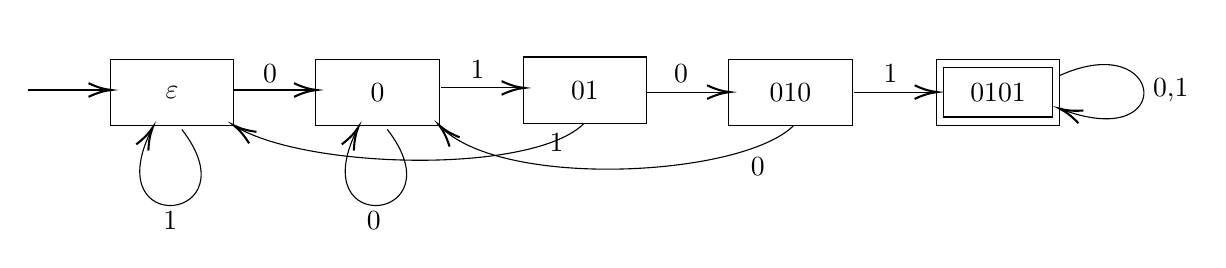
\begin{tikzpicture}[x=0.75pt,y=0.75pt,yscale=-1,xscale=1]
		%uncomment if require: \path (0,273.1999988555908); %set diagram left start at 0, and has height of 273.1999988555908
		
		%Shape: Rectangle [id:dp956976788795576] 
		\draw   (493.5,60) -- (546,60) -- (546,83.91) -- (493.5,83.91) -- cycle ;
		%Shape: Rectangle [id:dp8420859467362585] 
		\draw   (191,56) -- (250.5,56) -- (250.5,87.91) -- (191,87.91) -- cycle ;
		%Straight Lines [id:da5058522979107305] 
		\draw    (151.5,70.91) -- (189.5,70.91) ;
		\draw [shift={(191.5,70.91)}, rotate = 180] [color={rgb, 255:red, 0; green, 0; blue, 0 }  ][line width=0.75]    (10.93,-3.29) .. controls (6.95,-1.4) and (3.31,-0.3) .. (0,0) .. controls (3.31,0.3) and (6.95,1.4) .. (10.93,3.29)   ;
		
		%Shape: Rectangle [id:dp14240592094191928] 
		\draw   (291,55) -- (350.5,55) -- (350.5,86.91) -- (291,86.91) -- cycle ;
		%Straight Lines [id:da8400508696340678] 
		\draw    (251.5,69.91) -- (289.5,69.91) ;
		\draw [shift={(291.5,69.91)}, rotate = 180] [color={rgb, 255:red, 0; green, 0; blue, 0 }  ][line width=0.75]    (10.93,-3.29) .. controls (6.95,-1.4) and (3.31,-0.3) .. (0,0) .. controls (3.31,0.3) and (6.95,1.4) .. (10.93,3.29)   ;
		
		%Curve Lines [id:da3929647914483967] 
		\draw    (549.5,63.91) .. controls (599.99,41.14) and (606.38,100.69) .. (551.19,80.54) ;
		\draw [shift={(549.5,79.91)}, rotate = 381.1] [color={rgb, 255:red, 0; green, 0; blue, 0 }  ][line width=0.75]    (10.93,-3.29) .. controls (6.95,-1.4) and (3.31,-0.3) .. (0,0) .. controls (3.31,0.3) and (6.95,1.4) .. (10.93,3.29)   ;
		
		%Curve Lines [id:da43209873002088006] 
		\draw    (225.5,89.91) .. controls (260.15,134.46) and (185.03,142.74) .. (210.69,90.51) ;
		\draw [shift={(211.5,88.91)}, rotate = 477.41] [color={rgb, 255:red, 0; green, 0; blue, 0 }  ][line width=0.75]    (10.93,-3.29) .. controls (6.95,-1.4) and (3.31,-0.3) .. (0,0) .. controls (3.31,0.3) and (6.95,1.4) .. (10.93,3.29)   ;
		
		%Shape: Rectangle [id:dp9254601209026325] 
		\draw   (390,56) -- (449.5,56) -- (449.5,87.91) -- (390,87.91) -- cycle ;
		%Straight Lines [id:da5368673556619235] 
		\draw    (350.5,71.91) -- (388.5,71.91) ;
		\draw [shift={(390.5,71.91)}, rotate = 180] [color={rgb, 255:red, 0; green, 0; blue, 0 }  ][line width=0.75]    (10.93,-3.29) .. controls (6.95,-1.4) and (3.31,-0.3) .. (0,0) .. controls (3.31,0.3) and (6.95,1.4) .. (10.93,3.29)   ;
		
		%Shape: Rectangle [id:dp09868809673865675] 
		\draw   (490,56) -- (549.5,56) -- (549.5,87.91) -- (490,87.91) -- cycle ;
		%Straight Lines [id:da5198608402177753] 
		\draw    (450.5,71.91) -- (488.5,71.91) ;
		\draw [shift={(490.5,71.91)}, rotate = 180] [color={rgb, 255:red, 0; green, 0; blue, 0 }  ][line width=0.75]    (10.93,-3.29) .. controls (6.95,-1.4) and (3.31,-0.3) .. (0,0) .. controls (3.31,0.3) and (6.95,1.4) .. (10.93,3.29)   ;
		
		%Curve Lines [id:da16178621977035013] 
		\draw    (320.3,87) .. controls (295.67,111.63) and (187.61,109.08) .. (153.03,88.84) ;
		\draw [shift={(151.5,87.91)}, rotate = 392.75] [color={rgb, 255:red, 0; green, 0; blue, 0 }  ][line width=0.75]    (10.93,-3.29) .. controls (6.95,-1.4) and (3.31,-0.3) .. (0,0) .. controls (3.31,0.3) and (6.95,1.4) .. (10.93,3.29)   ;
		
		%Curve Lines [id:da38464073621417727] 
		\draw    (421.3,88) .. controls (396.67,112.63) and (282.79,118.82) .. (251.85,89.28) ;
		\draw [shift={(250.5,87.91)}, rotate = 407.19] [color={rgb, 255:red, 0; green, 0; blue, 0 }  ][line width=0.75]    (10.93,-3.29) .. controls (6.95,-1.4) and (3.31,-0.3) .. (0,0) .. controls (3.31,0.3) and (6.95,1.4) .. (10.93,3.29)   ;
		
		%Shape: Rectangle [id:dp7772611499680067] 
		\draw   (92,56) -- (151.5,56) -- (151.5,87.91) -- (92,87.91) -- cycle ;
		%Straight Lines [id:da3541280054643685] 
		\draw    (52.5,70.91) -- (90.5,70.91) ;
		\draw [shift={(92.5,70.91)}, rotate = 180] [color={rgb, 255:red, 0; green, 0; blue, 0 }  ][line width=0.75]    (10.93,-3.29) .. controls (6.95,-1.4) and (3.31,-0.3) .. (0,0) .. controls (3.31,0.3) and (6.95,1.4) .. (10.93,3.29)   ;
		
		%Curve Lines [id:da38525068704112164] 
		\draw    (126.5,89.91) .. controls (161.15,134.46) and (86.03,142.74) .. (111.69,90.51) ;
		\draw [shift={(112.5,88.91)}, rotate = 477.41] [color={rgb, 255:red, 0; green, 0; blue, 0 }  ][line width=0.75]    (10.93,-3.29) .. controls (6.95,-1.4) and (3.31,-0.3) .. (0,0) .. controls (3.31,0.3) and (6.95,1.4) .. (10.93,3.29)   ;
		
		% Text Node
		\draw (269,61) node  [align=left] {1};
		% Text Node
		\draw (603,71) node  [align=left] {0,1};
		% Text Node
		\draw (219,134) node  [align=left] {0};
		% Text Node
		\draw (220.75,71.95) node  [align=left] {0};
		% Text Node
		\draw (320.75,70.95) node  [align=left] {01};
		% Text Node
		\draw (367,63) node  [align=left] {0};
		% Text Node
		\draw (419.75,71.95) node  [align=left] {010};
		% Text Node
		\draw (468,63) node  [align=left] {1};
		% Text Node
		\draw (519.75,71.95) node  [align=left] {0101};
		% Text Node
		\draw (307,96) node  [align=left] {1};
		% Text Node
		\draw (404,108) node  [align=left] {0};
		% Text Node
		\draw (121,134) node  [align=left] {1};
		% Text Node
		\draw (121.75,71.95) node  [align=left] {$\varepsilon$};
		% Text Node
		\draw (169,63) node  [align=left] {0};
		
		\end{tikzpicture}

	\item[(c)]	~

		\tikzset{every picture/.style={line width=0.75pt}} %set default line width to 0.75pt        
		
		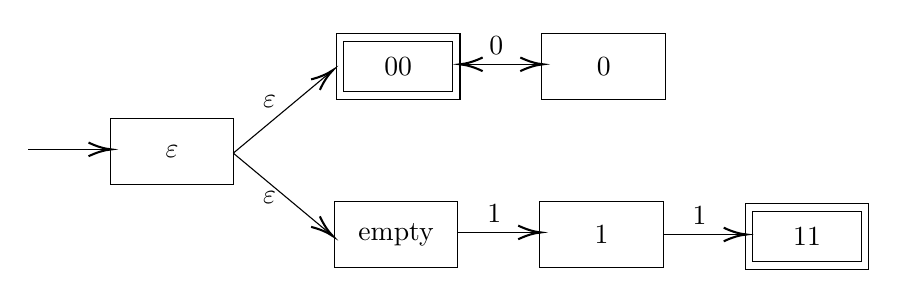
\begin{tikzpicture}[x=0.75pt,y=0.75pt,yscale=-1,xscale=1]
		%uncomment if require: \path (0,164.19998168945312); %set diagram left start at 0, and has height of 164.19998168945312
		
		%Straight Lines [id:da2147801922445769] 
		\draw    (233.3,87.2) -- (279.76,48.48) ;
		\draw [shift={(281.3,47.2)}, rotate = 500.19] [color={rgb, 255:red, 0; green, 0; blue, 0 }  ][line width=0.75]    (10.93,-3.29) .. controls (6.95,-1.4) and (3.31,-0.3) .. (0,0) .. controls (3.31,0.3) and (6.95,1.4) .. (10.93,3.29)   ;
		
		%Shape: Rectangle [id:dp015566963644975118] 
		\draw   (174,70.49) -- (233.5,70.49) -- (233.5,102.4) -- (174,102.4) -- cycle ;
		%Straight Lines [id:da4547714154764648] 
		\draw    (134.5,85.4) -- (172.5,85.4) ;
		\draw [shift={(174.5,85.4)}, rotate = 180] [color={rgb, 255:red, 0; green, 0; blue, 0 }  ][line width=0.75]    (10.93,-3.29) .. controls (6.95,-1.4) and (3.31,-0.3) .. (0,0) .. controls (3.31,0.3) and (6.95,1.4) .. (10.93,3.29)   ;
		
		%Shape: Rectangle [id:dp5784096082058308] 
		\draw   (283,29.49) -- (342.5,29.49) -- (342.5,61.4) -- (283,61.4) -- cycle ;
		%Shape: Rectangle [id:dp6845641115978134] 
		\draw   (382,29.49) -- (441.5,29.49) -- (441.5,61.4) -- (382,61.4) -- cycle ;
		%Straight Lines [id:da17704547499299772] 
		\draw    (344.5,44.4) -- (380.5,44.4) ;
		\draw [shift={(382.5,44.4)}, rotate = 180] [color={rgb, 255:red, 0; green, 0; blue, 0 }  ][line width=0.75]    (10.93,-3.29) .. controls (6.95,-1.4) and (3.31,-0.3) .. (0,0) .. controls (3.31,0.3) and (6.95,1.4) .. (10.93,3.29)   ;
		\draw [shift={(342.5,44.4)}, rotate = 0] [color={rgb, 255:red, 0; green, 0; blue, 0 }  ][line width=0.75]    (10.93,-3.29) .. controls (6.95,-1.4) and (3.31,-0.3) .. (0,0) .. controls (3.31,0.3) and (6.95,1.4) .. (10.93,3.29)   ;
		%Shape: Rectangle [id:dp5293293026901218] 
		\draw   (286.5,33.49) -- (339,33.49) -- (339,57.4) -- (286.5,57.4) -- cycle ;
		%Shape: Rectangle [id:dp060295452305052955] 
		\draw   (282,110.49) -- (341.5,110.49) -- (341.5,142.4) -- (282,142.4) -- cycle ;
		%Shape: Rectangle [id:dp2010494677144834] 
		\draw   (381,110.49) -- (440.5,110.49) -- (440.5,142.4) -- (381,142.4) -- cycle ;
		%Straight Lines [id:da947374916925185] 
		\draw    (341.5,125.4) -- (379.5,125.4) ;
		\draw [shift={(381.5,125.4)}, rotate = 180] [color={rgb, 255:red, 0; green, 0; blue, 0 }  ][line width=0.75]    (10.93,-3.29) .. controls (6.95,-1.4) and (3.31,-0.3) .. (0,0) .. controls (3.31,0.3) and (6.95,1.4) .. (10.93,3.29)   ;
		
		%Shape: Rectangle [id:dp9908026737785851] 
		\draw   (480,111.49) -- (539.5,111.49) -- (539.5,143.4) -- (480,143.4) -- cycle ;
		%Straight Lines [id:da016820912912296704] 
		\draw    (440.5,126.4) -- (478.5,126.4) ;
		\draw [shift={(480.5,126.4)}, rotate = 180] [color={rgb, 255:red, 0; green, 0; blue, 0 }  ][line width=0.75]    (10.93,-3.29) .. controls (6.95,-1.4) and (3.31,-0.3) .. (0,0) .. controls (3.31,0.3) and (6.95,1.4) .. (10.93,3.29)   ;
		
		%Shape: Rectangle [id:dp8268540717015087] 
		\draw   (483.5,115.49) -- (536,115.49) -- (536,139.4) -- (483.5,139.4) -- cycle ;
		%Straight Lines [id:da06621572069765569] 
		\draw    (233.3,87.2) -- (279.76,125.92) ;
		\draw [shift={(281.3,127.2)}, rotate = 219.81] [color={rgb, 255:red, 0; green, 0; blue, 0 }  ][line width=0.75]    (10.93,-3.29) .. controls (6.95,-1.4) and (3.31,-0.3) .. (0,0) .. controls (3.31,0.3) and (6.95,1.4) .. (10.93,3.29)   ;
		
		% Text Node
		\draw (203.75,86.45) node  [align=left] {$\varepsilon$};
		% Text Node
		\draw (312.75,45.45) node  [align=left] {00};
		% Text Node
		\draw (360,35.49) node  [align=left] {0};
		% Text Node
		\draw (411.75,45.45) node  [align=left] {0};
		% Text Node
		\draw (311.75,126.45) node  [align=left] {empty};
		% Text Node
		\draw (359,116.49) node  [align=left] {1};
		% Text Node
		\draw (410.75,126.45) node  [align=left] {1};
		% Text Node
		\draw (458,117.49) node  [align=left] {1};
		% Text Node
		\draw (509.75,127.45) node  [align=left] {11};
		% Text Node
		\draw (250.75,62.45) node  [align=left] {$\varepsilon$};
		% Text Node
		\draw (250.75,108.45) node  [align=left] {$\varepsilon$};
		
		\end{tikzpicture}

	\item[(d)]	~

		\tikzset{every picture/.style={line width=0.75pt}} %set default line width to 0.75pt        
		
		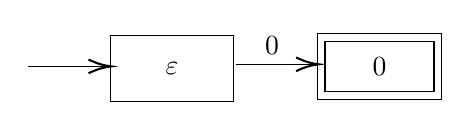
\begin{tikzpicture}[x=0.75pt,y=0.75pt,yscale=-1,xscale=1]
		%uncomment if require: \path (0,155.39999389648438); %set diagram left start at 0, and has height of 155.39999389648438
		
		%Shape: Rectangle [id:dp2228945460909495] 
		\draw   (258,50.49) -- (317.5,50.49) -- (317.5,82.4) -- (258,82.4) -- cycle ;
		%Straight Lines [id:da8142704276173571] 
		\draw    (218.5,65.4) -- (256.5,65.4) ;
		\draw [shift={(258.5,65.4)}, rotate = 180] [color={rgb, 255:red, 0; green, 0; blue, 0 }  ][line width=0.75]    (10.93,-3.29) .. controls (6.95,-1.4) and (3.31,-0.3) .. (0,0) .. controls (3.31,0.3) and (6.95,1.4) .. (10.93,3.29)   ;
		
		%Shape: Rectangle [id:dp19384573068998678] 
		\draw   (358,49.49) -- (417.5,49.49) -- (417.5,81.4) -- (358,81.4) -- cycle ;
		%Straight Lines [id:da13703081151443586] 
		\draw    (318.5,64.4) -- (356.5,64.4) ;
		\draw [shift={(358.5,64.4)}, rotate = 180] [color={rgb, 255:red, 0; green, 0; blue, 0 }  ][line width=0.75]    (10.93,-3.29) .. controls (6.95,-1.4) and (3.31,-0.3) .. (0,0) .. controls (3.31,0.3) and (6.95,1.4) .. (10.93,3.29)   ;
		
		%Shape: Rectangle [id:dp5622587101284653] 
		\draw   (361.5,53.49) -- (414,53.49) -- (414,77.4) -- (361.5,77.4) -- cycle ;
		
		% Text Node
		\draw (336,55.49) node  [align=left] {0};
		% Text Node
		\draw (287.75,66.45) node  [align=left] {$\varepsilon$};
		% Text Node
		\draw (387.75,65.45) node  [align=left] {0};
		
		\end{tikzpicture}

	\item[(e)]	~

		\tikzset{every picture/.style={line width=0.75pt}} %set default line width to 0.75pt        
		
		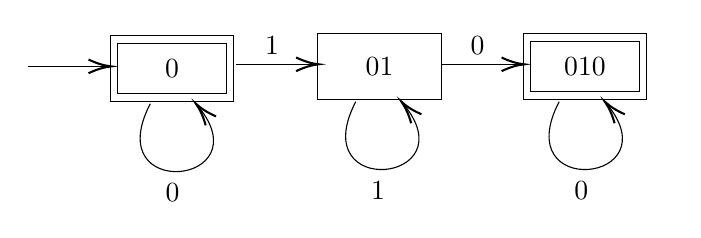
\begin{tikzpicture}[x=0.75pt,y=0.75pt,yscale=-1,xscale=1]
		%uncomment if require: \path (0,155.39999389648438); %set diagram left start at 0, and has height of 155.39999389648438
		
		%Shape: Rectangle [id:dp3596513615295296] 
		\draw   (258,50.49) -- (317.5,50.49) -- (317.5,82.4) -- (258,82.4) -- cycle ;
		%Straight Lines [id:da42685765935441666] 
		\draw    (218.5,65.4) -- (256.5,65.4) ;
		\draw [shift={(258.5,65.4)}, rotate = 180] [color={rgb, 255:red, 0; green, 0; blue, 0 }  ][line width=0.75]    (10.93,-3.29) .. controls (6.95,-1.4) and (3.31,-0.3) .. (0,0) .. controls (3.31,0.3) and (6.95,1.4) .. (10.93,3.29)   ;
		
		%Shape: Rectangle [id:dp9123641069822859] 
		\draw   (358,49.49) -- (417.5,49.49) -- (417.5,81.4) -- (358,81.4) -- cycle ;
		%Straight Lines [id:da022660673180210367] 
		\draw    (318.5,64.4) -- (356.5,64.4) ;
		\draw [shift={(358.5,64.4)}, rotate = 180] [color={rgb, 255:red, 0; green, 0; blue, 0 }  ][line width=0.75]    (10.93,-3.29) .. controls (6.95,-1.4) and (3.31,-0.3) .. (0,0) .. controls (3.31,0.3) and (6.95,1.4) .. (10.93,3.29)   ;
		
		%Shape: Rectangle [id:dp9305498611162519] 
		\draw   (457,49.49) -- (516.5,49.49) -- (516.5,81.4) -- (457,81.4) -- cycle ;
		%Straight Lines [id:da5865362276433232] 
		\draw    (417.5,64.4) -- (455.5,64.4) ;
		\draw [shift={(457.5,64.4)}, rotate = 180] [color={rgb, 255:red, 0; green, 0; blue, 0 }  ][line width=0.75]    (10.93,-3.29) .. controls (6.95,-1.4) and (3.31,-0.3) .. (0,0) .. controls (3.31,0.3) and (6.95,1.4) .. (10.93,3.29)   ;
		
		%Shape: Rectangle [id:dp17098001570204557] 
		\draw   (460.5,53.49) -- (513,53.49) -- (513,77.4) -- (460.5,77.4) -- cycle ;
		%Shape: Rectangle [id:dp737254977863846] 
		\draw   (261.5,54.49) -- (314,54.49) -- (314,78.4) -- (261.5,78.4) -- cycle ;
		%Curve Lines [id:da4902205046285282] 
		\draw    (277.3,83.4) .. controls (252.55,130.92) and (331.69,122.57) .. (300.29,84.56) ;
		\draw [shift={(299.3,83.4)}, rotate = 408.91999999999996] [color={rgb, 255:red, 0; green, 0; blue, 0 }  ][line width=0.75]    (10.93,-3.29) .. controls (6.95,-1.4) and (3.31,-0.3) .. (0,0) .. controls (3.31,0.3) and (6.95,1.4) .. (10.93,3.29)   ;
		
		%Curve Lines [id:da28876534153596656] 
		\draw    (376.3,82.4) .. controls (351.55,129.92) and (430.69,121.57) .. (399.29,83.56) ;
		\draw [shift={(398.3,82.4)}, rotate = 408.91999999999996] [color={rgb, 255:red, 0; green, 0; blue, 0 }  ][line width=0.75]    (10.93,-3.29) .. controls (6.95,-1.4) and (3.31,-0.3) .. (0,0) .. controls (3.31,0.3) and (6.95,1.4) .. (10.93,3.29)   ;
		
		%Curve Lines [id:da6921631984544991] 
		\draw    (474.3,82.4) .. controls (449.55,129.92) and (528.69,121.57) .. (497.29,83.56) ;
		\draw [shift={(496.3,82.4)}, rotate = 408.91999999999996] [color={rgb, 255:red, 0; green, 0; blue, 0 }  ][line width=0.75]    (10.93,-3.29) .. controls (6.95,-1.4) and (3.31,-0.3) .. (0,0) .. controls (3.31,0.3) and (6.95,1.4) .. (10.93,3.29)   ;
		
		% Text Node
		\draw (336,55.49) node  [align=left] {1};
		% Text Node
		\draw (287.75,66.45) node  [align=left] {0};
		% Text Node
		\draw (387.75,65.45) node  [align=left] {01};
		% Text Node
		\draw (435,55.49) node  [align=left] {0};
		% Text Node
		\draw (486.75,65.45) node  [align=left] {010};
		% Text Node
		\draw (288,126) node  [align=left] {0};
		% Text Node
		\draw (387,125) node  [align=left] {1};
		% Text Node
		\draw (485,125) node  [align=left] {0};
		
		\end{tikzpicture}

	\item[(g)]	~

		\tikzset{every picture/.style={line width=0.75pt}} %set default line width to 0.75pt        
		
		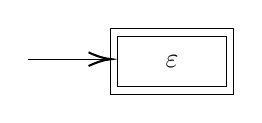
\begin{tikzpicture}[x=0.75pt,y=0.75pt,yscale=-1,xscale=1]
		%uncomment if require: \path (0,155.39999389648438); %set diagram left start at 0, and has height of 155.39999389648438
		
		%Shape: Rectangle [id:dp38100451904075605] 
		\draw   (258,50.49) -- (317.5,50.49) -- (317.5,82.4) -- (258,82.4) -- cycle ;
		%Straight Lines [id:da36220091684228195] 
		\draw    (218.5,65.4) -- (256.5,65.4) ;
		\draw [shift={(258.5,65.4)}, rotate = 180] [color={rgb, 255:red, 0; green, 0; blue, 0 }  ][line width=0.75]    (10.93,-3.29) .. controls (6.95,-1.4) and (3.31,-0.3) .. (0,0) .. controls (3.31,0.3) and (6.95,1.4) .. (10.93,3.29)   ;
		
		%Shape: Rectangle [id:dp8419819688166574] 
		\draw   (261.5,54.49) -- (314,54.49) -- (314,78.4) -- (261.5,78.4) -- cycle ;
		
		% Text Node
		\draw (287.75,66.45) node  [align=left] {$\varepsilon$};
		
		\end{tikzpicture}

	\item[(h)]	~

		\tikzset{every picture/.style={line width=0.75pt}} %set default line width to 0.75pt        
		
		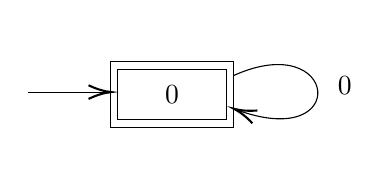
\begin{tikzpicture}[x=0.75pt,y=0.75pt,yscale=-1,xscale=1]
		%uncomment if require: \path (0,155.39999389648438); %set diagram left start at 0, and has height of 155.39999389648438
		
		%Shape: Rectangle [id:dp408724305705624] 
		\draw   (258,50.49) -- (317.5,50.49) -- (317.5,82.4) -- (258,82.4) -- cycle ;
		%Straight Lines [id:da9153452366594566] 
		\draw    (218.5,65.4) -- (256.5,65.4) ;
		\draw [shift={(258.5,65.4)}, rotate = 180] [color={rgb, 255:red, 0; green, 0; blue, 0 }  ][line width=0.75]    (10.93,-3.29) .. controls (6.95,-1.4) and (3.31,-0.3) .. (0,0) .. controls (3.31,0.3) and (6.95,1.4) .. (10.93,3.29)   ;
		
		%Shape: Rectangle [id:dp7221384319280304] 
		\draw   (261.5,54.49) -- (314,54.49) -- (314,78.4) -- (261.5,78.4) -- cycle ;
		%Curve Lines [id:da8810497058067093] 
		\draw    (317.5,57.4) .. controls (367.99,34.63) and (374.38,94.19) .. (319.19,74.04) ;
		\draw [shift={(317.5,73.4)}, rotate = 381.1] [color={rgb, 255:red, 0; green, 0; blue, 0 }  ][line width=0.75]    (10.93,-3.29) .. controls (6.95,-1.4) and (3.31,-0.3) .. (0,0) .. controls (3.31,0.3) and (6.95,1.4) .. (10.93,3.29)   ;
		
		% Text Node
		\draw (287.75,66.45) node  [align=left] {0};
		% Text Node
		\draw (371,62.49) node  [align=left] {0};
		
		\end{tikzpicture}

\end{enumerate}

\begin{problem}{1.8}
\end{problem}
\begin{enumerate}
	\item[(a)]	~

		\tikzset{every picture/.style={line width=0.75pt}} %set default line width to 0.75pt        
		
		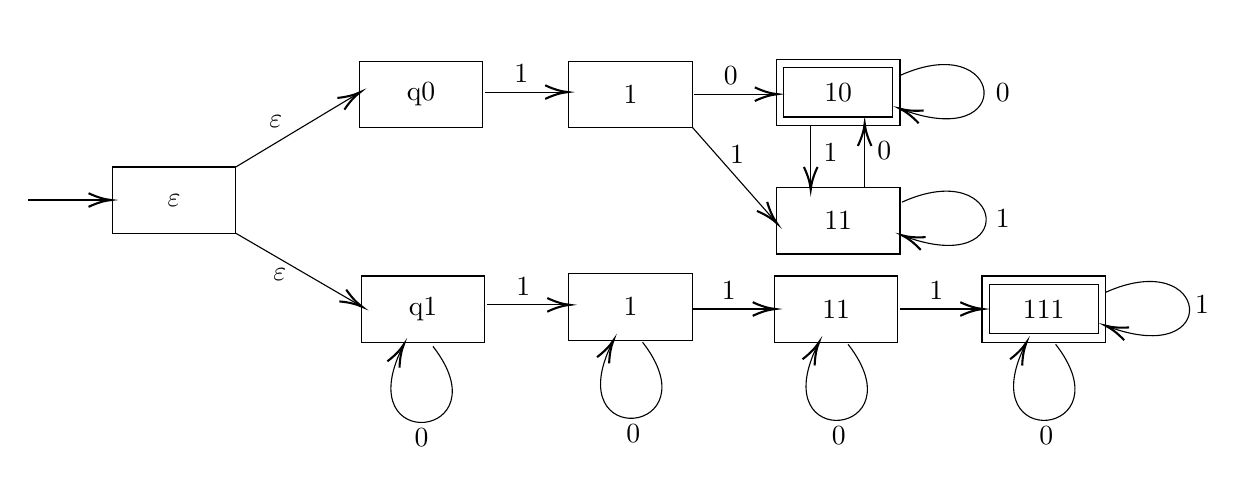
\begin{tikzpicture}[x=0.75pt,y=0.75pt,yscale=-1,xscale=1]
		%uncomment if require: \path (0,590.5625); %set diagram left start at 0, and has height of 590.5625
		
		%Shape: Rectangle [id:dp6962149588076394] 
		\draw   (239,152.49) -- (298.5,152.49) -- (298.5,184.4) -- (239,184.4) -- cycle ;
		%Straight Lines [id:da7691807332531746] 
		\draw    (179.5,203.49) -- (237.79,168.43) ;
		\draw [shift={(239.5,167.4)}, rotate = 508.97] [color={rgb, 255:red, 0; green, 0; blue, 0 }  ][line width=0.75]    (10.93,-3.29) .. controls (6.95,-1.4) and (3.31,-0.3) .. (0,0) .. controls (3.31,0.3) and (6.95,1.4) .. (10.93,3.29)   ;
		
		%Shape: Rectangle [id:dp36485373891091655] 
		\draw   (340,152.49) -- (399.5,152.49) -- (399.5,184.4) -- (340,184.4) -- cycle ;
		%Shape: Rectangle [id:dp9006830278402134] 
		\draw   (440,151.49) -- (499.5,151.49) -- (499.5,183.4) -- (440,183.4) -- cycle ;
		%Straight Lines [id:da230904712968804] 
		\draw    (400.5,168.4) -- (438.5,168.4) ;
		\draw [shift={(440.5,168.4)}, rotate = 180] [color={rgb, 255:red, 0; green, 0; blue, 0 }  ][line width=0.75]    (10.93,-3.29) .. controls (6.95,-1.4) and (3.31,-0.3) .. (0,0) .. controls (3.31,0.3) and (6.95,1.4) .. (10.93,3.29)   ;
		
		%Shape: Rectangle [id:dp2247382105625464] 
		\draw   (440,213.49) -- (499.5,213.49) -- (499.5,245.4) -- (440,245.4) -- cycle ;
		%Straight Lines [id:da2732146118751646] 
		\draw    (399.5,184.4) -- (438.98,229.19) ;
		\draw [shift={(440.3,230.69)}, rotate = 228.61] [color={rgb, 255:red, 0; green, 0; blue, 0 }  ][line width=0.75]    (10.93,-3.29) .. controls (6.95,-1.4) and (3.31,-0.3) .. (0,0) .. controls (3.31,0.3) and (6.95,1.4) .. (10.93,3.29)   ;
		
		%Straight Lines [id:da21947112881464403] 
		\draw    (482.5,184.4) -- (482.5,213.4) ;
		
		\draw [shift={(482.5,182.4)}, rotate = 90] [color={rgb, 255:red, 0; green, 0; blue, 0 }  ][line width=0.75]    (10.93,-3.29) .. controls (6.95,-1.4) and (3.31,-0.3) .. (0,0) .. controls (3.31,0.3) and (6.95,1.4) .. (10.93,3.29)   ;
		%Straight Lines [id:da14491121134595852] 
		\draw    (456.5,183.4) -- (456.5,212.4) ;
		\draw [shift={(456.5,214.4)}, rotate = 270] [color={rgb, 255:red, 0; green, 0; blue, 0 }  ][line width=0.75]    (10.93,-3.29) .. controls (6.95,-1.4) and (3.31,-0.3) .. (0,0) .. controls (3.31,0.3) and (6.95,1.4) .. (10.93,3.29)   ;
		
		%Curve Lines [id:da6691329136881574] 
		\draw    (499.5,159.4) .. controls (549.99,136.63) and (556.38,196.19) .. (501.19,176.04) ;
		\draw [shift={(499.5,175.4)}, rotate = 381.1] [color={rgb, 255:red, 0; green, 0; blue, 0 }  ][line width=0.75]    (10.93,-3.29) .. controls (6.95,-1.4) and (3.31,-0.3) .. (0,0) .. controls (3.31,0.3) and (6.95,1.4) .. (10.93,3.29)   ;
		
		%Curve Lines [id:da1451689803454992] 
		\draw    (500.5,220.4) .. controls (550.99,197.63) and (557.38,257.19) .. (502.19,237.04) ;
		\draw [shift={(500.5,236.4)}, rotate = 381.1] [color={rgb, 255:red, 0; green, 0; blue, 0 }  ][line width=0.75]    (10.93,-3.29) .. controls (6.95,-1.4) and (3.31,-0.3) .. (0,0) .. controls (3.31,0.3) and (6.95,1.4) .. (10.93,3.29)   ;
		
		%Shape: Rectangle [id:dp6617430630180456] 
		\draw   (443.5,155.49) -- (496,155.49) -- (496,179.4) -- (443.5,179.4) -- cycle ;
		%Shape: Rectangle [id:dp016433216855628263] 
		\draw   (542.5,260) -- (595,260) -- (595,283.91) -- (542.5,283.91) -- cycle ;
		%Shape: Rectangle [id:dp9022262185160514] 
		\draw   (240,256) -- (299.5,256) -- (299.5,287.91) -- (240,287.91) -- cycle ;
		%Straight Lines [id:da5787327843338388] 
		\draw    (179.5,235.4) -- (238.77,269.9) ;
		\draw [shift={(240.5,270.91)}, rotate = 210.2] [color={rgb, 255:red, 0; green, 0; blue, 0 }  ][line width=0.75]    (10.93,-3.29) .. controls (6.95,-1.4) and (3.31,-0.3) .. (0,0) .. controls (3.31,0.3) and (6.95,1.4) .. (10.93,3.29)   ;
		
		%Shape: Rectangle [id:dp9521717434366117] 
		\draw   (340,255) -- (399.5,255) -- (399.5,286.91) -- (340,286.91) -- cycle ;
		%Straight Lines [id:da3494396501091639] 
		\draw    (300.5,269.91) -- (338.5,269.91) ;
		\draw [shift={(340.5,269.91)}, rotate = 180] [color={rgb, 255:red, 0; green, 0; blue, 0 }  ][line width=0.75]    (10.93,-3.29) .. controls (6.95,-1.4) and (3.31,-0.3) .. (0,0) .. controls (3.31,0.3) and (6.95,1.4) .. (10.93,3.29)   ;
		
		%Curve Lines [id:da6258089591287197] 
		\draw    (598.5,263.91) .. controls (648.99,241.14) and (655.38,300.69) .. (600.19,280.54) ;
		\draw [shift={(598.5,279.91)}, rotate = 381.1] [color={rgb, 255:red, 0; green, 0; blue, 0 }  ][line width=0.75]    (10.93,-3.29) .. controls (6.95,-1.4) and (3.31,-0.3) .. (0,0) .. controls (3.31,0.3) and (6.95,1.4) .. (10.93,3.29)   ;
		
		%Curve Lines [id:da910174735008118] 
		\draw    (274.5,289.91) .. controls (309.15,334.46) and (234.03,342.74) .. (259.69,290.51) ;
		\draw [shift={(260.5,288.91)}, rotate = 477.41] [color={rgb, 255:red, 0; green, 0; blue, 0 }  ][line width=0.75]    (10.93,-3.29) .. controls (6.95,-1.4) and (3.31,-0.3) .. (0,0) .. controls (3.31,0.3) and (6.95,1.4) .. (10.93,3.29)   ;
		
		%Curve Lines [id:da6709564789050213] 
		\draw    (375.5,287.91) .. controls (410.15,332.46) and (335.03,340.74) .. (360.69,288.51) ;
		\draw [shift={(361.5,286.91)}, rotate = 477.41] [color={rgb, 255:red, 0; green, 0; blue, 0 }  ][line width=0.75]    (10.93,-3.29) .. controls (6.95,-1.4) and (3.31,-0.3) .. (0,0) .. controls (3.31,0.3) and (6.95,1.4) .. (10.93,3.29)   ;
		
		%Shape: Rectangle [id:dp8737219113079928] 
		\draw   (439,256) -- (498.5,256) -- (498.5,287.91) -- (439,287.91) -- cycle ;
		%Straight Lines [id:da3665856317225338] 
		\draw    (399.5,271.91) -- (437.5,271.91) ;
		\draw [shift={(439.5,271.91)}, rotate = 180] [color={rgb, 255:red, 0; green, 0; blue, 0 }  ][line width=0.75]    (10.93,-3.29) .. controls (6.95,-1.4) and (3.31,-0.3) .. (0,0) .. controls (3.31,0.3) and (6.95,1.4) .. (10.93,3.29)   ;
		
		%Curve Lines [id:da3072939873057112] 
		\draw    (474.5,288.91) .. controls (509.15,333.46) and (434.03,341.74) .. (459.69,289.51) ;
		\draw [shift={(460.5,287.91)}, rotate = 477.41] [color={rgb, 255:red, 0; green, 0; blue, 0 }  ][line width=0.75]    (10.93,-3.29) .. controls (6.95,-1.4) and (3.31,-0.3) .. (0,0) .. controls (3.31,0.3) and (6.95,1.4) .. (10.93,3.29)   ;
		
		%Shape: Rectangle [id:dp531253052617823] 
		\draw   (539,256) -- (598.5,256) -- (598.5,287.91) -- (539,287.91) -- cycle ;
		%Straight Lines [id:da3715624332912093] 
		\draw    (499.5,271.91) -- (537.5,271.91) ;
		\draw [shift={(539.5,271.91)}, rotate = 180] [color={rgb, 255:red, 0; green, 0; blue, 0 }  ][line width=0.75]    (10.93,-3.29) .. controls (6.95,-1.4) and (3.31,-0.3) .. (0,0) .. controls (3.31,0.3) and (6.95,1.4) .. (10.93,3.29)   ;
		
		%Curve Lines [id:da07735142336538603] 
		\draw    (574.5,288.91) .. controls (609.15,333.46) and (534.03,341.74) .. (559.69,289.51) ;
		\draw [shift={(560.5,287.91)}, rotate = 477.41] [color={rgb, 255:red, 0; green, 0; blue, 0 }  ][line width=0.75]    (10.93,-3.29) .. controls (6.95,-1.4) and (3.31,-0.3) .. (0,0) .. controls (3.31,0.3) and (6.95,1.4) .. (10.93,3.29)   ;
		
		%Straight Lines [id:da12190332921874258] 
		\draw    (299.5,167.4) -- (337.5,167.4) ;
		\draw [shift={(339.5,167.4)}, rotate = 180] [color={rgb, 255:red, 0; green, 0; blue, 0 }  ][line width=0.75]    (10.93,-3.29) .. controls (6.95,-1.4) and (3.31,-0.3) .. (0,0) .. controls (3.31,0.3) and (6.95,1.4) .. (10.93,3.29)   ;
		
		%Shape: Rectangle [id:dp38701919765060455] 
		\draw   (120,203.49) -- (179.5,203.49) -- (179.5,235.4) -- (120,235.4) -- cycle ;
		%Straight Lines [id:da6325419370723289] 
		\draw    (79.5,219.4) -- (117.5,219.4) ;
		\draw [shift={(119.5,219.4)}, rotate = 180] [color={rgb, 255:red, 0; green, 0; blue, 0 }  ][line width=0.75]    (10.93,-3.29) .. controls (6.95,-1.4) and (3.31,-0.3) .. (0,0) .. controls (3.31,0.3) and (6.95,1.4) .. (10.93,3.29)   ;
		
		% Text Node
		\draw (418,159.49) node  [align=left] {0};
		% Text Node
		\draw (268.75,168.45) node  [align=left] {q0};
		% Text Node
		\draw (369.75,168.45) node  [align=left] {1};
		% Text Node
		\draw (469.75,167.45) node  [align=left] {10};
		% Text Node
		\draw (469.75,229.45) node  [align=left] {11};
		% Text Node
		\draw (421,197.49) node  [align=left] {1};
		% Text Node
		\draw (492,195.49) node  [align=left] {0};
		% Text Node
		\draw (466,196.49) node  [align=left] {1};
		% Text Node
		\draw (549,167.49) node  [align=left] {0};
		% Text Node
		\draw (549,228.49) node  [align=left] {1};
		% Text Node
		\draw (318,261) node  [align=left] {1};
		% Text Node
		\draw (645,270) node  [align=left] {1};
		% Text Node
		\draw (269,334) node  [align=left] {0};
		% Text Node
		\draw (371,332) node  [align=left] {0};
		% Text Node
		\draw (269.75,271.95) node  [align=left] {q1};
		% Text Node
		\draw (369.75,270.95) node  [align=left] {1};
		% Text Node
		\draw (417,263) node  [align=left] {1};
		% Text Node
		\draw (470,333) node  [align=left] {0};
		% Text Node
		\draw (468.75,271.95) node  [align=left] {11};
		% Text Node
		\draw (517,263) node  [align=left] {1};
		% Text Node
		\draw (570,333) node  [align=left] {0};
		% Text Node
		\draw (568.75,271.95) node  [align=left] {111};
		% Text Node
		\draw (317,158.49) node  [align=left] {1};
		% Text Node
		\draw (149.75,219.45) node  [align=left] {$\varepsilon$};
		% Text Node
		\draw (198.75,181.45) node  [align=left] {$\varepsilon$};
		% Text Node
		\draw (200.75,255.45) node  [align=left] {$\varepsilon$};
		
		\end{tikzpicture}

	\item[(b)]	~

	\tikzset{every picture/.style={line width=0.75pt}} %set default line width to 0.75pt        
	
	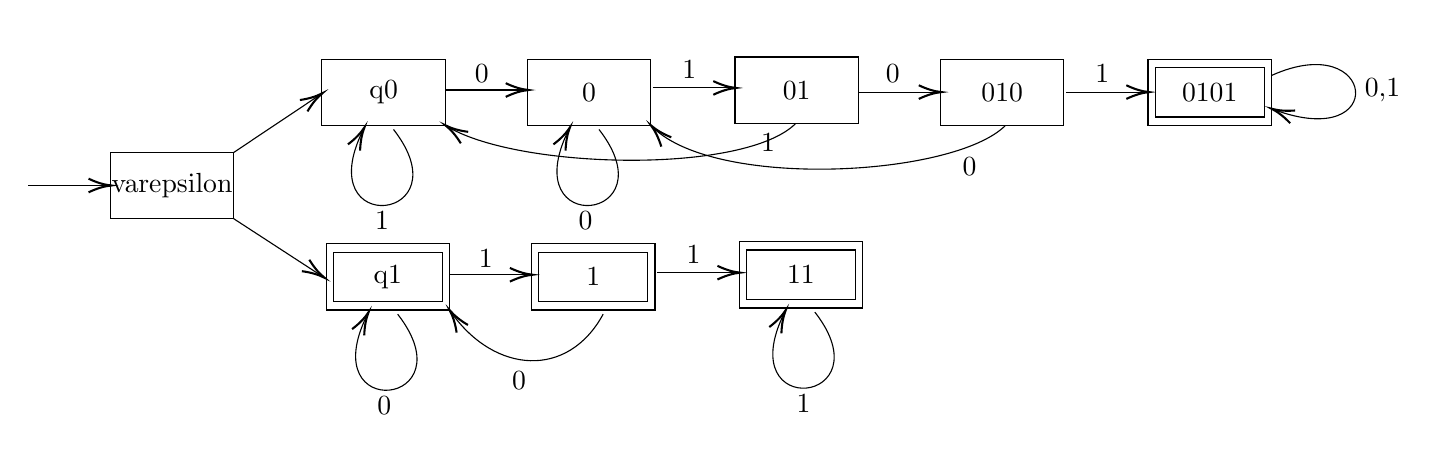
\begin{tikzpicture}[x=0.75pt,y=0.75pt,yscale=-1,xscale=1]
	%uncomment if require: \path (0,210.39999389648438); %set diagram left start at 0, and has height of 210.39999389648438
	
	%Shape: Rectangle [id:dp8224465004417729] 
	\draw   (537.5,22) -- (590,22) -- (590,45.91) -- (537.5,45.91) -- cycle ;
	%Shape: Rectangle [id:dp41448950949330365] 
	\draw   (235,18) -- (294.5,18) -- (294.5,49.91) -- (235,49.91) -- cycle ;
	%Straight Lines [id:da9207386165616951] 
	\draw    (195.5,32.91) -- (233.5,32.91) ;
	\draw [shift={(235.5,32.91)}, rotate = 180] [color={rgb, 255:red, 0; green, 0; blue, 0 }  ][line width=0.75]    (10.93,-3.29) .. controls (6.95,-1.4) and (3.31,-0.3) .. (0,0) .. controls (3.31,0.3) and (6.95,1.4) .. (10.93,3.29)   ;
	
	%Shape: Rectangle [id:dp7881299594534485] 
	\draw   (335,17) -- (394.5,17) -- (394.5,48.91) -- (335,48.91) -- cycle ;
	%Straight Lines [id:da13719952172135108] 
	\draw    (295.5,31.91) -- (333.5,31.91) ;
	\draw [shift={(335.5,31.91)}, rotate = 180] [color={rgb, 255:red, 0; green, 0; blue, 0 }  ][line width=0.75]    (10.93,-3.29) .. controls (6.95,-1.4) and (3.31,-0.3) .. (0,0) .. controls (3.31,0.3) and (6.95,1.4) .. (10.93,3.29)   ;
	
	%Curve Lines [id:da2847971479448197] 
	\draw    (593.5,25.91) .. controls (643.99,3.14) and (650.38,62.69) .. (595.19,42.54) ;
	\draw [shift={(593.5,41.91)}, rotate = 381.1] [color={rgb, 255:red, 0; green, 0; blue, 0 }  ][line width=0.75]    (10.93,-3.29) .. controls (6.95,-1.4) and (3.31,-0.3) .. (0,0) .. controls (3.31,0.3) and (6.95,1.4) .. (10.93,3.29)   ;
	
	%Curve Lines [id:da38670254174428975] 
	\draw    (269.5,51.91) .. controls (304.15,96.46) and (229.03,104.74) .. (254.69,52.51) ;
	\draw [shift={(255.5,50.91)}, rotate = 477.41] [color={rgb, 255:red, 0; green, 0; blue, 0 }  ][line width=0.75]    (10.93,-3.29) .. controls (6.95,-1.4) and (3.31,-0.3) .. (0,0) .. controls (3.31,0.3) and (6.95,1.4) .. (10.93,3.29)   ;
	
	%Shape: Rectangle [id:dp7445306277643156] 
	\draw   (434,18) -- (493.5,18) -- (493.5,49.91) -- (434,49.91) -- cycle ;
	%Straight Lines [id:da6943858180390376] 
	\draw    (394.5,33.91) -- (432.5,33.91) ;
	\draw [shift={(434.5,33.91)}, rotate = 180] [color={rgb, 255:red, 0; green, 0; blue, 0 }  ][line width=0.75]    (10.93,-3.29) .. controls (6.95,-1.4) and (3.31,-0.3) .. (0,0) .. controls (3.31,0.3) and (6.95,1.4) .. (10.93,3.29)   ;
	
	%Shape: Rectangle [id:dp3563909923663917] 
	\draw   (534,18) -- (593.5,18) -- (593.5,49.91) -- (534,49.91) -- cycle ;
	%Straight Lines [id:da6396084172922765] 
	\draw    (494.5,33.91) -- (532.5,33.91) ;
	\draw [shift={(534.5,33.91)}, rotate = 180] [color={rgb, 255:red, 0; green, 0; blue, 0 }  ][line width=0.75]    (10.93,-3.29) .. controls (6.95,-1.4) and (3.31,-0.3) .. (0,0) .. controls (3.31,0.3) and (6.95,1.4) .. (10.93,3.29)   ;
	
	%Curve Lines [id:da20058879807883834] 
	\draw    (364.3,49) .. controls (339.67,73.63) and (231.61,71.08) .. (197.03,50.84) ;
	\draw [shift={(195.5,49.91)}, rotate = 392.75] [color={rgb, 255:red, 0; green, 0; blue, 0 }  ][line width=0.75]    (10.93,-3.29) .. controls (6.95,-1.4) and (3.31,-0.3) .. (0,0) .. controls (3.31,0.3) and (6.95,1.4) .. (10.93,3.29)   ;
	
	%Curve Lines [id:da8780710027451988] 
	\draw    (465.3,50) .. controls (440.67,74.63) and (326.79,80.82) .. (295.85,51.28) ;
	\draw [shift={(294.5,49.91)}, rotate = 407.19] [color={rgb, 255:red, 0; green, 0; blue, 0 }  ][line width=0.75]    (10.93,-3.29) .. controls (6.95,-1.4) and (3.31,-0.3) .. (0,0) .. controls (3.31,0.3) and (6.95,1.4) .. (10.93,3.29)   ;
	
	%Shape: Rectangle [id:dp3919514081318305] 
	\draw   (136,18) -- (195.5,18) -- (195.5,49.91) -- (136,49.91) -- cycle ;
	%Curve Lines [id:da8743562819608273] 
	\draw    (170.5,51.91) .. controls (205.15,96.46) and (130.03,104.74) .. (155.69,52.51) ;
	\draw [shift={(156.5,50.91)}, rotate = 477.41] [color={rgb, 255:red, 0; green, 0; blue, 0 }  ][line width=0.75]    (10.93,-3.29) .. controls (6.95,-1.4) and (3.31,-0.3) .. (0,0) .. controls (3.31,0.3) and (6.95,1.4) .. (10.93,3.29)   ;
	
	%Straight Lines [id:da614779030671945] 
	\draw    (93.5,63) -- (134.64,35.51) ;
	\draw [shift={(136.3,34.4)}, rotate = 506.25] [color={rgb, 255:red, 0; green, 0; blue, 0 }  ][line width=0.75]    (10.93,-3.29) .. controls (6.95,-1.4) and (3.31,-0.3) .. (0,0) .. controls (3.31,0.3) and (6.95,1.4) .. (10.93,3.29)   ;
	
	%Shape: Rectangle [id:dp7040609026783278] 
	\draw   (34,63) -- (93.5,63) -- (93.5,94.91) -- (34,94.91) -- cycle ;
	%Straight Lines [id:da1584936164891837] 
	\draw    (93.5,94.91) -- (135.62,122.31) ;
	\draw [shift={(137.3,123.4)}, rotate = 213.05] [color={rgb, 255:red, 0; green, 0; blue, 0 }  ][line width=0.75]    (10.93,-3.29) .. controls (6.95,-1.4) and (3.31,-0.3) .. (0,0) .. controls (3.31,0.3) and (6.95,1.4) .. (10.93,3.29)   ;
	
	%Straight Lines [id:da5078636889526362] 
	\draw    (-5.5,78.91) -- (32.5,78.91) ;
	\draw [shift={(34.5,78.91)}, rotate = 180] [color={rgb, 255:red, 0; green, 0; blue, 0 }  ][line width=0.75]    (10.93,-3.29) .. controls (6.95,-1.4) and (3.31,-0.3) .. (0,0) .. controls (3.31,0.3) and (6.95,1.4) .. (10.93,3.29)   ;
	
	%Shape: Rectangle [id:dp863323504401752] 
	\draw   (340.5,110) -- (393,110) -- (393,133.91) -- (340.5,133.91) -- cycle ;
	%Shape: Rectangle [id:dp07900971921418853] 
	\draw   (237,107) -- (296.5,107) -- (296.5,138.91) -- (237,138.91) -- cycle ;
	%Straight Lines [id:da900400064761506] 
	\draw    (197.5,121.91) -- (235.5,121.91) ;
	\draw [shift={(237.5,121.91)}, rotate = 180] [color={rgb, 255:red, 0; green, 0; blue, 0 }  ][line width=0.75]    (10.93,-3.29) .. controls (6.95,-1.4) and (3.31,-0.3) .. (0,0) .. controls (3.31,0.3) and (6.95,1.4) .. (10.93,3.29)   ;
	
	%Shape: Rectangle [id:dp6050932893385321] 
	\draw   (337,106) -- (396.5,106) -- (396.5,137.91) -- (337,137.91) -- cycle ;
	%Straight Lines [id:da7969085799522302] 
	\draw    (297.5,120.91) -- (335.5,120.91) ;
	\draw [shift={(337.5,120.91)}, rotate = 180] [color={rgb, 255:red, 0; green, 0; blue, 0 }  ][line width=0.75]    (10.93,-3.29) .. controls (6.95,-1.4) and (3.31,-0.3) .. (0,0) .. controls (3.31,0.3) and (6.95,1.4) .. (10.93,3.29)   ;
	
	%Curve Lines [id:da7241941613641896] 
	\draw    (271.5,140.91) .. controls (254.56,172.12) and (219.38,169.68) .. (198.45,140.27) ;
	\draw [shift={(197.5,138.91)}, rotate = 415.88] [color={rgb, 255:red, 0; green, 0; blue, 0 }  ][line width=0.75]    (10.93,-3.29) .. controls (6.95,-1.4) and (3.31,-0.3) .. (0,0) .. controls (3.31,0.3) and (6.95,1.4) .. (10.93,3.29)   ;
	
	%Shape: Rectangle [id:dp9353566110819995] 
	\draw   (138,107) -- (197.5,107) -- (197.5,138.91) -- (138,138.91) -- cycle ;
	%Curve Lines [id:da7568371291471723] 
	\draw    (172.5,140.91) .. controls (207.15,185.46) and (132.03,193.74) .. (157.69,141.51) ;
	\draw [shift={(158.5,139.91)}, rotate = 477.41] [color={rgb, 255:red, 0; green, 0; blue, 0 }  ][line width=0.75]    (10.93,-3.29) .. controls (6.95,-1.4) and (3.31,-0.3) .. (0,0) .. controls (3.31,0.3) and (6.95,1.4) .. (10.93,3.29)   ;
	
	%Curve Lines [id:da4128731318624801] 
	\draw    (373.5,139.91) .. controls (408.15,184.46) and (333.03,192.74) .. (358.69,140.51) ;
	\draw [shift={(359.5,138.91)}, rotate = 477.41] [color={rgb, 255:red, 0; green, 0; blue, 0 }  ][line width=0.75]    (10.93,-3.29) .. controls (6.95,-1.4) and (3.31,-0.3) .. (0,0) .. controls (3.31,0.3) and (6.95,1.4) .. (10.93,3.29)   ;
	
	%Shape: Rectangle [id:dp5967711454586182] 
	\draw   (240.5,111) -- (293,111) -- (293,134.91) -- (240.5,134.91) -- cycle ;
	%Shape: Rectangle [id:dp3479211353029761] 
	\draw   (141.5,111) -- (194,111) -- (194,134.91) -- (141.5,134.91) -- cycle ;
	
	% Text Node
	\draw (313,23) node  [align=left] {1};
	% Text Node
	\draw (647,33) node  [align=left] {0,1};
	% Text Node
	\draw (263,96) node  [align=left] {0};
	% Text Node
	\draw (264.75,33.95) node  [align=left] {0};
	% Text Node
	\draw (364.75,32.95) node  [align=left] {01};
	% Text Node
	\draw (411,25) node  [align=left] {0};
	% Text Node
	\draw (463.75,33.95) node  [align=left] {010};
	% Text Node
	\draw (512,25) node  [align=left] {1};
	% Text Node
	\draw (563.75,33.95) node  [align=left] {0101};
	% Text Node
	\draw (351,58) node  [align=left] {1};
	% Text Node
	\draw (448,70) node  [align=left] {0};
	% Text Node
	\draw (165,96) node  [align=left] {1};
	% Text Node
	\draw (165.75,33.95) node  [align=left] {q0};
	% Text Node
	\draw (213,25) node  [align=left] {0};
	% Text Node
	\draw (63.75,78.95) node  [align=left] {varepsilon};
	% Text Node
	\draw (315,112) node  [align=left] {1};
	% Text Node
	\draw (266.75,122.95) node  [align=left] {1};
	% Text Node
	\draw (366.75,121.95) node  [align=left] {11};
	% Text Node
	\draw (167.75,122.95) node  [align=left] {q1};
	% Text Node
	\draw (215,114) node  [align=left] {1};
	% Text Node
	\draw (166,185) node  [align=left] {0};
	% Text Node
	\draw (231,173) node  [align=left] {0};
	% Text Node
	\draw (368,184) node  [align=left] {1};
	
	\end{tikzpicture}

\end{enumerate}

\begin{problem}{1.9}
\end{problem}
\begin{enumerate}
	\item[(a)]	~

		\tikzset{every picture/.style={line width=0.75pt}} %set default line width to 0.75pt        
		
		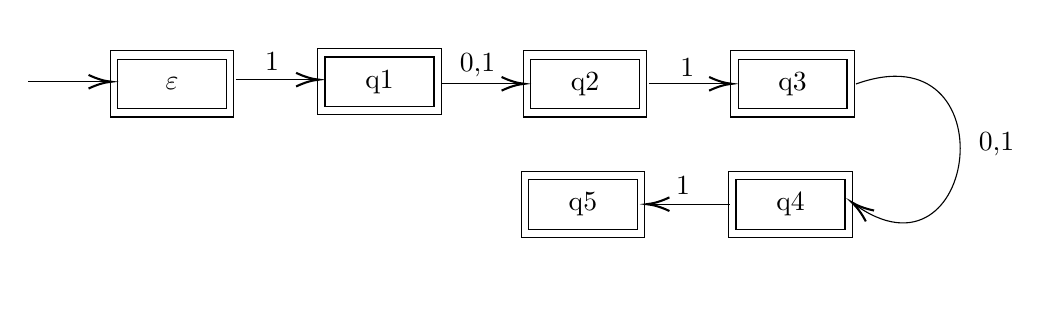
\begin{tikzpicture}[x=0.75pt,y=0.75pt,yscale=-1,xscale=1]
		%uncomment if require: \path (0,146.59999084472656); %set diagram left start at 0, and has height of 146.59999084472656
		
		%Shape: Rectangle [id:dp8975684438198428] 
		\draw   (117,44) -- (176.5,44) -- (176.5,75.91) -- (117,75.91) -- cycle ;
		%Straight Lines [id:da2712051773138626] 
		\draw    (77.5,58.91) -- (115.5,58.91) ;
		\draw [shift={(117.5,58.91)}, rotate = 180] [color={rgb, 255:red, 0; green, 0; blue, 0 }  ][line width=0.75]    (10.93,-3.29) .. controls (6.95,-1.4) and (3.31,-0.3) .. (0,0) .. controls (3.31,0.3) and (6.95,1.4) .. (10.93,3.29)   ;
		
		%Shape: Rectangle [id:dp33683585681177286] 
		\draw   (217,43) -- (276.5,43) -- (276.5,74.91) -- (217,74.91) -- cycle ;
		%Straight Lines [id:da45304839344611914] 
		\draw    (177.5,57.91) -- (215.5,57.91) ;
		\draw [shift={(217.5,57.91)}, rotate = 180] [color={rgb, 255:red, 0; green, 0; blue, 0 }  ][line width=0.75]    (10.93,-3.29) .. controls (6.95,-1.4) and (3.31,-0.3) .. (0,0) .. controls (3.31,0.3) and (6.95,1.4) .. (10.93,3.29)   ;
		
		%Shape: Rectangle [id:dp2341034552919432] 
		\draw   (316,44) -- (375.5,44) -- (375.5,75.91) -- (316,75.91) -- cycle ;
		%Straight Lines [id:da07383052769435694] 
		\draw    (276.5,59.91) -- (314.5,59.91) ;
		\draw [shift={(316.5,59.91)}, rotate = 180] [color={rgb, 255:red, 0; green, 0; blue, 0 }  ][line width=0.75]    (10.93,-3.29) .. controls (6.95,-1.4) and (3.31,-0.3) .. (0,0) .. controls (3.31,0.3) and (6.95,1.4) .. (10.93,3.29)   ;
		
		%Shape: Rectangle [id:dp23595202967399675] 
		\draw   (416,44) -- (475.5,44) -- (475.5,75.91) -- (416,75.91) -- cycle ;
		%Straight Lines [id:da2963264460519148] 
		\draw    (376.5,59.91) -- (414.5,59.91) ;
		\draw [shift={(416.5,59.91)}, rotate = 180] [color={rgb, 255:red, 0; green, 0; blue, 0 }  ][line width=0.75]    (10.93,-3.29) .. controls (6.95,-1.4) and (3.31,-0.3) .. (0,0) .. controls (3.31,0.3) and (6.95,1.4) .. (10.93,3.29)   ;
		
		%Shape: Rectangle [id:dp919696802469623] 
		\draw   (315,102) -- (374.5,102) -- (374.5,133.91) -- (315,133.91) -- cycle ;
		%Shape: Rectangle [id:dp10598405901636543] 
		\draw   (415,102) -- (474.5,102) -- (474.5,133.91) -- (415,133.91) -- cycle ;
		%Straight Lines [id:da9441055820463098] 
		\draw    (377.5,117.91) -- (415.5,117.91) ;
		
		\draw [shift={(375.5,117.91)}, rotate = 0] [color={rgb, 255:red, 0; green, 0; blue, 0 }  ][line width=0.75]    (10.93,-3.29) .. controls (6.95,-1.4) and (3.31,-0.3) .. (0,0) .. controls (3.31,0.3) and (6.95,1.4) .. (10.93,3.29)   ;
		%Curve Lines [id:da3739544996827544] 
		\draw    (476.3,60) .. controls (550.92,33.13) and (535.46,161.7) .. (475.21,117.68) ;
		\draw [shift={(474.3,117)}, rotate = 397.02] [color={rgb, 255:red, 0; green, 0; blue, 0 }  ][line width=0.75]    (10.93,-3.29) .. controls (6.95,-1.4) and (3.31,-0.3) .. (0,0) .. controls (3.31,0.3) and (6.95,1.4) .. (10.93,3.29)   ;
		
		%Shape: Rectangle [id:dp40303518007315153] 
		\draw   (120.5,48) -- (173,48) -- (173,71.91) -- (120.5,71.91) -- cycle ;
		%Shape: Rectangle [id:dp5491515332410757] 
		\draw   (220.5,47) -- (273,47) -- (273,70.91) -- (220.5,70.91) -- cycle ;
		%Shape: Rectangle [id:dp600188427659125] 
		\draw   (319.5,48) -- (372,48) -- (372,71.91) -- (319.5,71.91) -- cycle ;
		%Shape: Rectangle [id:dp6922295857316167] 
		\draw   (419.5,48) -- (472,48) -- (472,71.91) -- (419.5,71.91) -- cycle ;
		%Shape: Rectangle [id:dp690876316419853] 
		\draw   (418.5,106) -- (471,106) -- (471,129.91) -- (418.5,129.91) -- cycle ;
		%Shape: Rectangle [id:dp10115588831452671] 
		\draw   (318.5,106) -- (371,106) -- (371,129.91) -- (318.5,129.91) -- cycle ;
		
		% Text Node
		\draw (195,49) node  [align=left] {1};
		% Text Node
		\draw (146.75,59.95) node  [align=left] {$\varepsilon$};
		% Text Node
		\draw (246.75,58.95) node  [align=left] {q1};
		% Text Node
		\draw (294,51) node  [align=left] {0,1};
		% Text Node
		\draw (345.75,59.95) node  [align=left] {q2};
		% Text Node
		\draw (445.75,59.95) node  [align=left] {q3};
		% Text Node
		\draw (344.75,117.95) node  [align=left] {q5};
		% Text Node
		\draw (393,109) node  [align=left] {1};
		% Text Node
		\draw (444.75,117.95) node  [align=left] {q4};
		% Text Node
		\draw (395,52) node  [align=left] {1};
		% Text Node
		\draw (544,89) node  [align=left] {0,1};
		
		\end{tikzpicture}

	\item[(b)]	Set cannot be empty while containing 1s. Set does not exist. 
\end{enumerate}

\begin{problem}{1.10}
\end{problem}
\begin{enumerate}
	\item[(a)]	~

		\tikzset{every picture/.style={line width=0.75pt}} %set default line width to 0.75pt        
		
		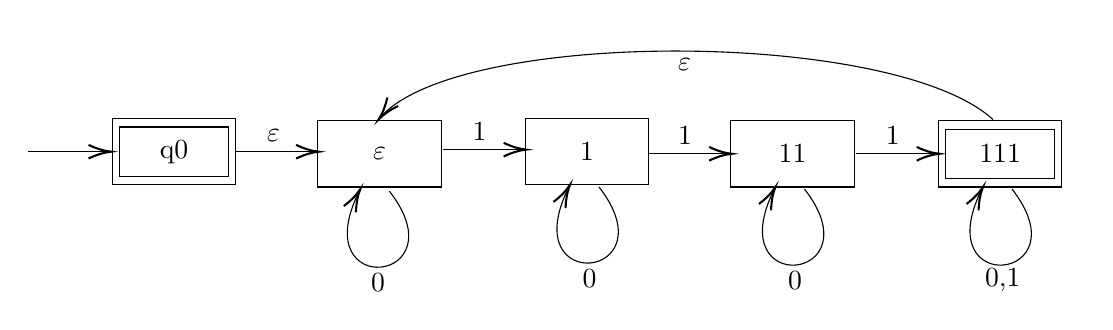
\begin{tikzpicture}[x=0.75pt,y=0.75pt,yscale=-1,xscale=1]
		%uncomment if require: \path (0,157.625); %set diagram left start at 0, and has height of 157.625
		
		%Shape: Rectangle [id:dp13808766013083318] 
		\draw   (529.5,63) -- (582,63) -- (582,86.91) -- (529.5,86.91) -- cycle ;
		%Shape: Rectangle [id:dp8816812491705055] 
		\draw   (227,59) -- (286.5,59) -- (286.5,90.91) -- (227,90.91) -- cycle ;
		%Straight Lines [id:da3055521905564551] 
		\draw    (187.5,73.91) -- (225.5,73.91) ;
		\draw [shift={(227.5,73.91)}, rotate = 180] [color={rgb, 255:red, 0; green, 0; blue, 0 }  ][line width=0.75]    (10.93,-3.29) .. controls (6.95,-1.4) and (3.31,-0.3) .. (0,0) .. controls (3.31,0.3) and (6.95,1.4) .. (10.93,3.29)   ;
		
		%Shape: Rectangle [id:dp348714108943482] 
		\draw   (327,58) -- (386.5,58) -- (386.5,89.91) -- (327,89.91) -- cycle ;
		%Straight Lines [id:da9323099822907939] 
		\draw    (287.5,72.91) -- (325.5,72.91) ;
		\draw [shift={(327.5,72.91)}, rotate = 180] [color={rgb, 255:red, 0; green, 0; blue, 0 }  ][line width=0.75]    (10.93,-3.29) .. controls (6.95,-1.4) and (3.31,-0.3) .. (0,0) .. controls (3.31,0.3) and (6.95,1.4) .. (10.93,3.29)   ;
		
		%Curve Lines [id:da7262978773237114] 
		\draw    (261.5,92.91) .. controls (296.15,137.46) and (221.03,145.74) .. (246.69,93.51) ;
		\draw [shift={(247.5,91.91)}, rotate = 477.41] [color={rgb, 255:red, 0; green, 0; blue, 0 }  ][line width=0.75]    (10.93,-3.29) .. controls (6.95,-1.4) and (3.31,-0.3) .. (0,0) .. controls (3.31,0.3) and (6.95,1.4) .. (10.93,3.29)   ;
		
		%Curve Lines [id:da10680745302935146] 
		\draw    (362.5,90.91) .. controls (397.15,135.46) and (322.03,143.74) .. (347.69,91.51) ;
		\draw [shift={(348.5,89.91)}, rotate = 477.41] [color={rgb, 255:red, 0; green, 0; blue, 0 }  ][line width=0.75]    (10.93,-3.29) .. controls (6.95,-1.4) and (3.31,-0.3) .. (0,0) .. controls (3.31,0.3) and (6.95,1.4) .. (10.93,3.29)   ;
		
		%Shape: Rectangle [id:dp6046879554443674] 
		\draw   (426,59) -- (485.5,59) -- (485.5,90.91) -- (426,90.91) -- cycle ;
		%Straight Lines [id:da688611769037289] 
		\draw    (386.5,74.91) -- (424.5,74.91) ;
		\draw [shift={(426.5,74.91)}, rotate = 180] [color={rgb, 255:red, 0; green, 0; blue, 0 }  ][line width=0.75]    (10.93,-3.29) .. controls (6.95,-1.4) and (3.31,-0.3) .. (0,0) .. controls (3.31,0.3) and (6.95,1.4) .. (10.93,3.29)   ;
		
		%Curve Lines [id:da24324012769080605] 
		\draw    (461.5,91.91) .. controls (496.15,136.46) and (421.03,144.74) .. (446.69,92.51) ;
		\draw [shift={(447.5,90.91)}, rotate = 477.41] [color={rgb, 255:red, 0; green, 0; blue, 0 }  ][line width=0.75]    (10.93,-3.29) .. controls (6.95,-1.4) and (3.31,-0.3) .. (0,0) .. controls (3.31,0.3) and (6.95,1.4) .. (10.93,3.29)   ;
		
		%Shape: Rectangle [id:dp5673977282360558] 
		\draw   (526,59) -- (585.5,59) -- (585.5,90.91) -- (526,90.91) -- cycle ;
		%Straight Lines [id:da9246844368686822] 
		\draw    (486.5,74.91) -- (524.5,74.91) ;
		\draw [shift={(526.5,74.91)}, rotate = 180] [color={rgb, 255:red, 0; green, 0; blue, 0 }  ][line width=0.75]    (10.93,-3.29) .. controls (6.95,-1.4) and (3.31,-0.3) .. (0,0) .. controls (3.31,0.3) and (6.95,1.4) .. (10.93,3.29)   ;
		
		%Shape: Rectangle [id:dp7939727601788034] 
		\draw   (128,58) -- (187.5,58) -- (187.5,89.91) -- (128,89.91) -- cycle ;
		%Shape: Rectangle [id:dp9798733476617041] 
		\draw   (131.5,62) -- (184,62) -- (184,85.91) -- (131.5,85.91) -- cycle ;
		%Straight Lines [id:da7216523332301343] 
		\draw    (87.5,73.91) -- (125.5,73.91) ;
		\draw [shift={(127.5,73.91)}, rotate = 180] [color={rgb, 255:red, 0; green, 0; blue, 0 }  ][line width=0.75]    (10.93,-3.29) .. controls (6.95,-1.4) and (3.31,-0.3) .. (0,0) .. controls (3.31,0.3) and (6.95,1.4) .. (10.93,3.29)   ;
		
		%Curve Lines [id:da46340782861532714] 
		\draw    (552.3,58.41) .. controls (504.78,14.85) and (295.54,14.42) .. (257.4,57.11) ;
		\draw [shift={(256.3,58.41)}, rotate = 308.5] [color={rgb, 255:red, 0; green, 0; blue, 0 }  ][line width=0.75]    (10.93,-3.29) .. controls (6.95,-1.4) and (3.31,-0.3) .. (0,0) .. controls (3.31,0.3) and (6.95,1.4) .. (10.93,3.29)   ;
		
		%Curve Lines [id:da4098958398699184] 
		\draw    (561.5,91.91) .. controls (596.15,136.46) and (521.03,144.74) .. (546.69,92.51) ;
		\draw [shift={(547.5,90.91)}, rotate = 477.41] [color={rgb, 255:red, 0; green, 0; blue, 0 }  ][line width=0.75]    (10.93,-3.29) .. controls (6.95,-1.4) and (3.31,-0.3) .. (0,0) .. controls (3.31,0.3) and (6.95,1.4) .. (10.93,3.29)   ;
		
		% Text Node
		\draw (305,64) node  [align=left] {1};
		% Text Node
		\draw (256,137) node  [align=left] {0};
		% Text Node
		\draw (358,135) node  [align=left] {0};
		% Text Node
		\draw (256.75,74.95) node  [align=left] {$\varepsilon$};
		% Text Node
		\draw (356.75,73.95) node  [align=left] {1};
		% Text Node
		\draw (404,66) node  [align=left] {1};
		% Text Node
		\draw (457,136) node  [align=left] {0};
		% Text Node
		\draw (455.75,74.95) node  [align=left] {11};
		% Text Node
		\draw (504,66) node  [align=left] {1};
		% Text Node
		\draw (555.75,74.95) node  [align=left] {111};
		% Text Node
		\draw (157.75,73.95) node  [align=left] {q0};
		% Text Node
		\draw (205.75,65.95) node  [align=left] {$\varepsilon$};
		% Text Node
		\draw (403.75,31.95) node  [align=left] {$\varepsilon$};
		% Text Node
		\draw (557,136) node  [align=left] {0,1};
		
		\end{tikzpicture}

	\item[(b)]	~

		\tikzset{every picture/.style={line width=0.75pt}} %set default line width to 0.75pt        
		
		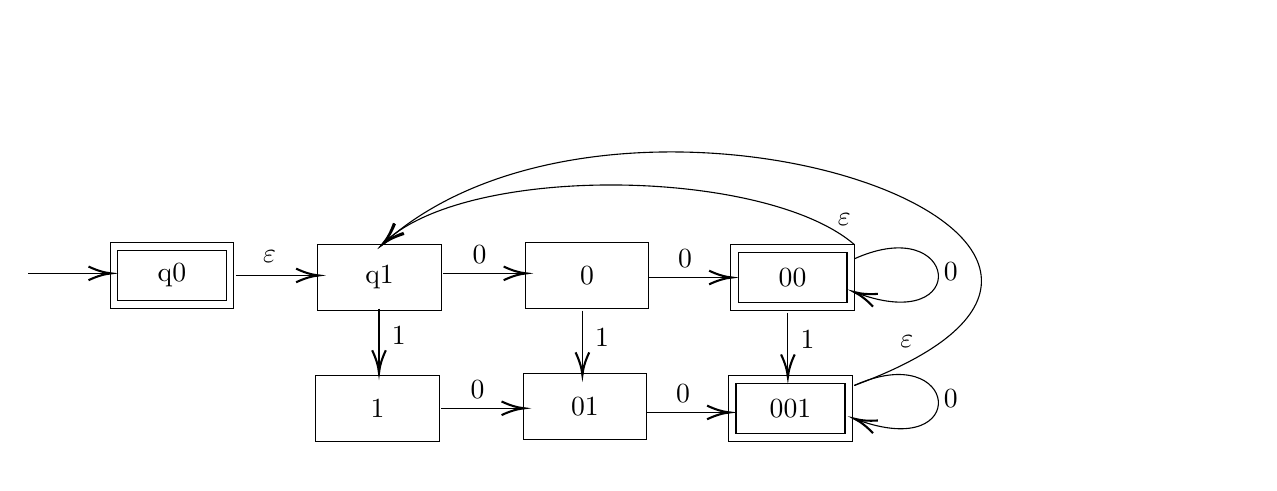
\begin{tikzpicture}[x=0.75pt,y=0.75pt,yscale=-1,xscale=1]
		%uncomment if require: \path (0,227.8000030517578); %set diagram left start at 0, and has height of 227.8000030517578
		
		%Shape: Rectangle [id:dp6471773519122883] 
		\draw   (239,68) -- (298.5,68) -- (298.5,99.91) -- (239,99.91) -- cycle ;
		%Straight Lines [id:da1229397015530933] 
		\draw    (199.5,82.91) -- (237.5,82.91) ;
		\draw [shift={(239.5,82.91)}, rotate = 180] [color={rgb, 255:red, 0; green, 0; blue, 0 }  ][line width=0.75]    (10.93,-3.29) .. controls (6.95,-1.4) and (3.31,-0.3) .. (0,0) .. controls (3.31,0.3) and (6.95,1.4) .. (10.93,3.29)   ;
		
		%Straight Lines [id:da4272367765855525] 
		\draw    (268.5,98.91) -- (268.5,127.91) ;
		\draw [shift={(268.5,129.91)}, rotate = 270] [color={rgb, 255:red, 0; green, 0; blue, 0 }  ][line width=0.75]    (10.93,-3.29) .. controls (6.95,-1.4) and (3.31,-0.3) .. (0,0) .. controls (3.31,0.3) and (6.95,1.4) .. (10.93,3.29)   ;
		
		%Shape: Rectangle [id:dp8521999903285014] 
		\draw   (339,67) -- (398.5,67) -- (398.5,98.91) -- (339,98.91) -- cycle ;
		%Straight Lines [id:da6358310085255237] 
		\draw    (299.5,81.91) -- (337.5,81.91) ;
		\draw [shift={(339.5,81.91)}, rotate = 180] [color={rgb, 255:red, 0; green, 0; blue, 0 }  ][line width=0.75]    (10.93,-3.29) .. controls (6.95,-1.4) and (3.31,-0.3) .. (0,0) .. controls (3.31,0.3) and (6.95,1.4) .. (10.93,3.29)   ;
		
		%Shape: Rectangle [id:dp8226291735117743] 
		\draw   (238,131) -- (297.5,131) -- (297.5,162.91) -- (238,162.91) -- cycle ;
		%Shape: Rectangle [id:dp14570693165153004] 
		\draw   (338,130) -- (397.5,130) -- (397.5,161.91) -- (338,161.91) -- cycle ;
		%Curve Lines [id:da7093513320481335] 
		\draw    (497.5,74.91) .. controls (547.99,52.14) and (554.38,111.69) .. (499.19,91.54) ;
		\draw [shift={(497.5,90.91)}, rotate = 381.1] [color={rgb, 255:red, 0; green, 0; blue, 0 }  ][line width=0.75]    (10.93,-3.29) .. controls (6.95,-1.4) and (3.31,-0.3) .. (0,0) .. controls (3.31,0.3) and (6.95,1.4) .. (10.93,3.29)   ;
		
		%Curve Lines [id:da9069451656992455] 
		\draw    (497.5,135.91) .. controls (547.99,113.14) and (554.38,172.69) .. (499.19,152.54) ;
		\draw [shift={(497.5,151.91)}, rotate = 381.1] [color={rgb, 255:red, 0; green, 0; blue, 0 }  ][line width=0.75]    (10.93,-3.29) .. controls (6.95,-1.4) and (3.31,-0.3) .. (0,0) .. controls (3.31,0.3) and (6.95,1.4) .. (10.93,3.29)   ;
		
		%Straight Lines [id:da3052114339515888] 
		\draw    (298.5,146.91) -- (336.5,146.91) ;
		\draw [shift={(338.5,146.91)}, rotate = 180] [color={rgb, 255:red, 0; green, 0; blue, 0 }  ][line width=0.75]    (10.93,-3.29) .. controls (6.95,-1.4) and (3.31,-0.3) .. (0,0) .. controls (3.31,0.3) and (6.95,1.4) .. (10.93,3.29)   ;
		
		%Straight Lines [id:da38406452739859476] 
		\draw    (366.5,99.91) -- (366.5,128.91) ;
		\draw [shift={(366.5,130.91)}, rotate = 270] [color={rgb, 255:red, 0; green, 0; blue, 0 }  ][line width=0.75]    (10.93,-3.29) .. controls (6.95,-1.4) and (3.31,-0.3) .. (0,0) .. controls (3.31,0.3) and (6.95,1.4) .. (10.93,3.29)   ;
		
		%Shape: Rectangle [id:dp6715099250875376] 
		\draw   (438,68) -- (497.5,68) -- (497.5,99.91) -- (438,99.91) -- cycle ;
		%Straight Lines [id:da679225729945349] 
		\draw    (398.5,83.91) -- (436.5,83.91) ;
		\draw [shift={(438.5,83.91)}, rotate = 180] [color={rgb, 255:red, 0; green, 0; blue, 0 }  ][line width=0.75]    (10.93,-3.29) .. controls (6.95,-1.4) and (3.31,-0.3) .. (0,0) .. controls (3.31,0.3) and (6.95,1.4) .. (10.93,3.29)   ;
		
		%Shape: Rectangle [id:dp6553607740426461] 
		\draw   (437,131) -- (496.5,131) -- (496.5,162.91) -- (437,162.91) -- cycle ;
		%Straight Lines [id:da32821325870787654] 
		\draw    (397.5,148.91) -- (435.5,148.91) ;
		\draw [shift={(437.5,148.91)}, rotate = 180] [color={rgb, 255:red, 0; green, 0; blue, 0 }  ][line width=0.75]    (10.93,-3.29) .. controls (6.95,-1.4) and (3.31,-0.3) .. (0,0) .. controls (3.31,0.3) and (6.95,1.4) .. (10.93,3.29)   ;
		
		%Straight Lines [id:da9575947555220381] 
		\draw    (465.5,100.91) -- (465.5,129.91) ;
		\draw [shift={(465.5,131.91)}, rotate = 270] [color={rgb, 255:red, 0; green, 0; blue, 0 }  ][line width=0.75]    (10.93,-3.29) .. controls (6.95,-1.4) and (3.31,-0.3) .. (0,0) .. controls (3.31,0.3) and (6.95,1.4) .. (10.93,3.29)   ;
		
		%Shape: Rectangle [id:dp05962098743662425] 
		\draw   (441.5,72) -- (494,72) -- (494,95.91) -- (441.5,95.91) -- cycle ;
		%Shape: Rectangle [id:dp1134432447009821] 
		\draw   (440.5,135) -- (493,135) -- (493,158.91) -- (440.5,158.91) -- cycle ;
		%Shape: Rectangle [id:dp570520730259048] 
		\draw   (139,67) -- (198.5,67) -- (198.5,98.91) -- (139,98.91) -- cycle ;
		%Straight Lines [id:da7031238056213704] 
		\draw    (99.5,81.91) -- (137.5,81.91) ;
		\draw [shift={(139.5,81.91)}, rotate = 180] [color={rgb, 255:red, 0; green, 0; blue, 0 }  ][line width=0.75]    (10.93,-3.29) .. controls (6.95,-1.4) and (3.31,-0.3) .. (0,0) .. controls (3.31,0.3) and (6.95,1.4) .. (10.93,3.29)   ;
		
		%Shape: Rectangle [id:dp6932548957619922] 
		\draw   (142.5,71) -- (195,71) -- (195,94.91) -- (142.5,94.91) -- cycle ;
		%Curve Lines [id:da23903443883459352] 
		\draw    (497.5,68) .. controls (454.73,31.17) and (312.19,28.84) .. (271.5,66.64) ;
		\draw [shift={(270.3,67.8)}, rotate = 315] [color={rgb, 255:red, 0; green, 0; blue, 0 }  ][line width=0.75]    (10.93,-3.29) .. controls (6.95,-1.4) and (3.31,-0.3) .. (0,0) .. controls (3.31,0.3) and (6.95,1.4) .. (10.93,3.29)   ;
		
		%Curve Lines [id:da9616969988803736] 
		\draw    (497.5,135.91) .. controls (687.5,65.91) and (385.3,-36.2) .. (270.3,67.8) ;
		\draw [shift={(270.3,67.8)}, rotate = 317.88] [color={rgb, 255:red, 0; green, 0; blue, 0 }  ][line width=0.75]    (10.93,-3.29) .. controls (6.95,-1.4) and (3.31,-0.3) .. (0,0) .. controls (3.31,0.3) and (6.95,1.4) .. (10.93,3.29)   ;
		
		% Text Node
		\draw (317,73) node  [align=left] {0};
		% Text Node
		\draw (316,138) node  [align=left] {0};
		% Text Node
		\draw (544,81) node  [align=left] {0};
		% Text Node
		\draw (544,142) node  [align=left] {0};
		% Text Node
		\draw (278,112) node  [align=left] {1};
		% Text Node
		\draw (376,113) node  [align=left] {1};
		% Text Node
		\draw (268.75,83.95) node  [align=left] {q1};
		% Text Node
		\draw (368.75,82.95) node  [align=left] {0};
		% Text Node
		\draw (267.75,146.95) node  [align=left] {1};
		% Text Node
		\draw (367.75,145.95) node  [align=left] {01};
		% Text Node
		\draw (416,75) node  [align=left] {0};
		% Text Node
		\draw (415,140) node  [align=left] {0};
		% Text Node
		\draw (475,114) node  [align=left] {1};
		% Text Node
		\draw (467.75,83.95) node  [align=left] {00};
		% Text Node
		\draw (466.75,146.95) node  [align=left] {001};
		% Text Node
		\draw (168.75,82.95) node  [align=left] {q0};
		% Text Node
		\draw (215.75,73.95) node  [align=left] {$\varepsilon$};
		% Text Node
		\draw (492.75,55.95) node  [align=left] {$\varepsilon$};
		% Text Node
		\draw (522.75,114.95) node  [align=left] {$\varepsilon$};
		
		\end{tikzpicture}

	\item[(c)]	~

		\tikzset{every picture/.style={line width=0.75pt}} %set default line width to 0.75pt        
		
		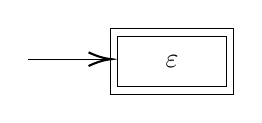
\begin{tikzpicture}[x=0.75pt,y=0.75pt,yscale=-1,xscale=1]
		%uncomment if require: \path (0,155.39999389648438); %set diagram left start at 0, and has height of 155.39999389648438
		
		%Shape: Rectangle [id:dp6935509719598922] 
		\draw   (334,55) -- (393.5,55) -- (393.5,86.91) -- (334,86.91) -- cycle ;
		%Straight Lines [id:da7417903660919858] 
		\draw    (294.5,69.91) -- (332.5,69.91) ;
		\draw [shift={(334.5,69.91)}, rotate = 180] [color={rgb, 255:red, 0; green, 0; blue, 0 }  ][line width=0.75]    (10.93,-3.29) .. controls (6.95,-1.4) and (3.31,-0.3) .. (0,0) .. controls (3.31,0.3) and (6.95,1.4) .. (10.93,3.29)   ;
		
		%Shape: Rectangle [id:dp25367308433805014] 
		\draw   (337.5,59) -- (390,59) -- (390,82.91) -- (337.5,82.91) -- cycle ;
		
		% Text Node
		\draw (363.75,70.95) node  [align=left] {$\varepsilon$};
		
		\end{tikzpicture}

\end{enumerate}

\begin{problem}{1.12}
\end{problem}
$D$ = $\{ \: \{\varepsilon, a, b, ba, bab\}, \{a, b\}, \delta, \varepsilon, \{b, ba\}\}$	\\
$\delta = 
\begin{array}{ c|c|c }
	 & a & b\\
	\hline
	\varepsilon & a & b\\
	\hline
	a & a & a\\
	\hline
	b & ba & b\\
	\hline
	ba & ba & bab\\
	\hline
	bab & bab & bab
\end{array}$\\
Regular expressio: D = $b^+a^*$

\begin{problem}{1.13}
\end{problem}

	\tikzset{every picture/.style={line width=0.75pt}} %set default line width to 0.75pt        
	
	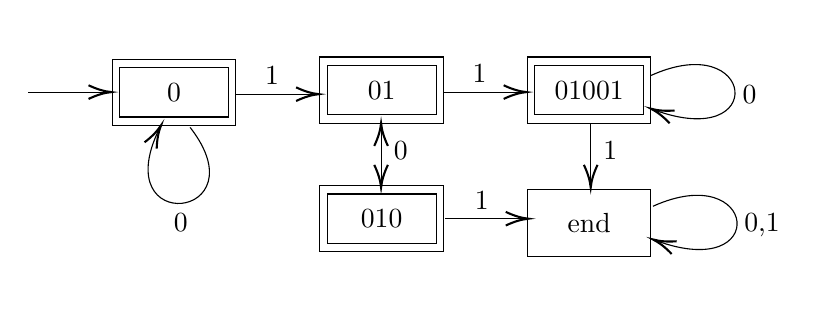
\begin{tikzpicture}[x=0.75pt,y=0.75pt,yscale=-1,xscale=1]
	%uncomment if require: \path (0,141.60000610351562); %set diagram left start at 0, and has height of 141.60000610351562
	
	%Shape: Rectangle [id:dp7729105648393069] 
	\draw   (194,22) -- (253.5,22) -- (253.5,53.91) -- (194,53.91) -- cycle ;
	%Shape: Rectangle [id:dp7511487359531526] 
	\draw   (294,21) -- (353.5,21) -- (353.5,52.91) -- (294,52.91) -- cycle ;
	%Straight Lines [id:da04244977475759937] 
	\draw    (153.5,37.91) -- (191.5,37.91) ;
	\draw [shift={(193.5,37.91)}, rotate = 180] [color={rgb, 255:red, 0; green, 0; blue, 0 }  ][line width=0.75]    (10.93,-3.29) .. controls (6.95,-1.4) and (3.31,-0.3) .. (0,0) .. controls (3.31,0.3) and (6.95,1.4) .. (10.93,3.29)   ;
	
	%Straight Lines [id:da7595251235691847] 
	\draw    (253.5,38.91) -- (291.5,38.91) ;
	\draw [shift={(293.5,38.91)}, rotate = 180] [color={rgb, 255:red, 0; green, 0; blue, 0 }  ][line width=0.75]    (10.93,-3.29) .. controls (6.95,-1.4) and (3.31,-0.3) .. (0,0) .. controls (3.31,0.3) and (6.95,1.4) .. (10.93,3.29)   ;
	
	%Shape: Rectangle [id:dp06238815529843511] 
	\draw   (294,83) -- (353.5,83) -- (353.5,114.91) -- (294,114.91) -- cycle ;
	%Shape: Rectangle [id:dp48008225015485806] 
	\draw   (297.5,25) -- (350,25) -- (350,48.91) -- (297.5,48.91) -- cycle ;
	%Curve Lines [id:da47837860959393463] 
	\draw    (231.5,54.91) .. controls (266.15,99.46) and (191.03,107.74) .. (216.69,55.51) ;
	\draw [shift={(217.5,53.91)}, rotate = 477.41] [color={rgb, 255:red, 0; green, 0; blue, 0 }  ][line width=0.75]    (10.93,-3.29) .. controls (6.95,-1.4) and (3.31,-0.3) .. (0,0) .. controls (3.31,0.3) and (6.95,1.4) .. (10.93,3.29)   ;
	
	%Shape: Rectangle [id:dp8793430998970824] 
	\draw   (394,21) -- (453.5,21) -- (453.5,52.91) -- (394,52.91) -- cycle ;
	%Shape: Rectangle [id:dp7425778948902579] 
	\draw   (397.5,25) -- (450,25) -- (450,48.91) -- (397.5,48.91) -- cycle ;
	%Curve Lines [id:da3870331480515412] 
	\draw    (453.5,29.91) .. controls (503.99,7.14) and (510.38,66.69) .. (455.19,46.54) ;
	\draw [shift={(453.5,45.91)}, rotate = 381.1] [color={rgb, 255:red, 0; green, 0; blue, 0 }  ][line width=0.75]    (10.93,-3.29) .. controls (6.95,-1.4) and (3.31,-0.3) .. (0,0) .. controls (3.31,0.3) and (6.95,1.4) .. (10.93,3.29)   ;
	
	%Shape: Rectangle [id:dp2583550122745184] 
	\draw   (197.5,26) -- (250,26) -- (250,49.91) -- (197.5,49.91) -- cycle ;
	%Shape: Rectangle [id:dp04979915907349053] 
	\draw   (297.5,87) -- (350,87) -- (350,110.91) -- (297.5,110.91) -- cycle ;
	%Straight Lines [id:da14338369735295253] 
	\draw    (323.5,54.91) -- (323.5,81.91) ;
	\draw [shift={(323.5,83.91)}, rotate = 270] [color={rgb, 255:red, 0; green, 0; blue, 0 }  ][line width=0.75]    (10.93,-3.29) .. controls (6.95,-1.4) and (3.31,-0.3) .. (0,0) .. controls (3.31,0.3) and (6.95,1.4) .. (10.93,3.29)   ;
	\draw [shift={(323.5,52.91)}, rotate = 90] [color={rgb, 255:red, 0; green, 0; blue, 0 }  ][line width=0.75]    (10.93,-3.29) .. controls (6.95,-1.4) and (3.31,-0.3) .. (0,0) .. controls (3.31,0.3) and (6.95,1.4) .. (10.93,3.29)   ;
	%Straight Lines [id:da2993075925041331] 
	\draw    (424.5,52.91) -- (424.5,81.91) ;
	\draw [shift={(424.5,83.91)}, rotate = 270] [color={rgb, 255:red, 0; green, 0; blue, 0 }  ][line width=0.75]    (10.93,-3.29) .. controls (6.95,-1.4) and (3.31,-0.3) .. (0,0) .. controls (3.31,0.3) and (6.95,1.4) .. (10.93,3.29)   ;
	
	%Shape: Rectangle [id:dp12700678408289523] 
	\draw   (394,85) -- (453.5,85) -- (453.5,116.91) -- (394,116.91) -- cycle ;
	%Straight Lines [id:da16923171475065346] 
	\draw    (353.5,37.91) -- (391.5,37.91) ;
	\draw [shift={(393.5,37.91)}, rotate = 180] [color={rgb, 255:red, 0; green, 0; blue, 0 }  ][line width=0.75]    (10.93,-3.29) .. controls (6.95,-1.4) and (3.31,-0.3) .. (0,0) .. controls (3.31,0.3) and (6.95,1.4) .. (10.93,3.29)   ;
	
	%Straight Lines [id:da990398661160595] 
	\draw    (354.5,98.91) -- (392.5,98.91) ;
	\draw [shift={(394.5,98.91)}, rotate = 180] [color={rgb, 255:red, 0; green, 0; blue, 0 }  ][line width=0.75]    (10.93,-3.29) .. controls (6.95,-1.4) and (3.31,-0.3) .. (0,0) .. controls (3.31,0.3) and (6.95,1.4) .. (10.93,3.29)   ;
	
	%Curve Lines [id:da5365566520968936] 
	\draw    (454.5,92.91) .. controls (504.99,70.14) and (511.38,129.69) .. (456.19,109.54) ;
	\draw [shift={(454.5,108.91)}, rotate = 381.1] [color={rgb, 255:red, 0; green, 0; blue, 0 }  ][line width=0.75]    (10.93,-3.29) .. controls (6.95,-1.4) and (3.31,-0.3) .. (0,0) .. controls (3.31,0.3) and (6.95,1.4) .. (10.93,3.29)   ;
	
	% Text Node
	\draw (323.75,36.95) node  [align=left] {01};
	% Text Node
	\draw (271,30) node  [align=left] {1};
	% Text Node
	\draw (223.75,37.95) node  [align=left] {0};
	% Text Node
	\draw (323.75,98.95) node  [align=left] {010};
	% Text Node
	\draw (227,101) node  [align=left] {0};
	% Text Node
	\draw (423.75,36.95) node  [align=left] {01001};
	% Text Node
	\draw (501,39) node  [align=left] {0};
	% Text Node
	\draw (333,66) node  [align=left] {0};
	% Text Node
	\draw (434,66) node  [align=left] {1};
	% Text Node
	\draw (423.75,100.95) node  [align=left] {end};
	% Text Node
	\draw (371,29) node  [align=left] {1};
	% Text Node
	\draw (372,90) node  [align=left] {1};
	% Text Node
	\draw (507,102) node  [align=left] {0,1};
	
	\end{tikzpicture}

\begin{problem}{1.16}
\end{problem}
\begin{enumerate}
	\item[(a)]	~

		\tikzset{every picture/.style={line width=0.75pt}} %set default line width to 0.75pt        
		
		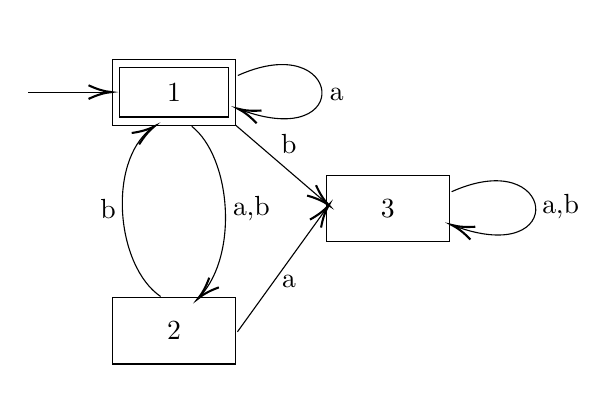
\begin{tikzpicture}[x=0.75pt,y=0.75pt,yscale=-1,xscale=1]
		%uncomment if require: \path (0,185.39999389648438); %set diagram left start at 0, and has height of 185.39999389648438
		
		%Curve Lines [id:da9727668282444577] 
		\draw    (277.5,18.91) .. controls (327.99,-3.86) and (334.38,55.69) .. (279.19,35.54) ;
		\draw [shift={(277.5,34.91)}, rotate = 381.1] [color={rgb, 255:red, 0; green, 0; blue, 0 }  ][line width=0.75]    (10.93,-3.29) .. controls (6.95,-1.4) and (3.31,-0.3) .. (0,0) .. controls (3.31,0.3) and (6.95,1.4) .. (10.93,3.29)   ;
		
		%Shape: Rectangle [id:dp9076494780480537] 
		\draw   (217,11) -- (276.5,11) -- (276.5,42.91) -- (217,42.91) -- cycle ;
		%Straight Lines [id:da7845140406636097] 
		\draw    (176.5,26.91) -- (214.5,26.91) ;
		\draw [shift={(216.5,26.91)}, rotate = 180] [color={rgb, 255:red, 0; green, 0; blue, 0 }  ][line width=0.75]    (10.93,-3.29) .. controls (6.95,-1.4) and (3.31,-0.3) .. (0,0) .. controls (3.31,0.3) and (6.95,1.4) .. (10.93,3.29)   ;
		
		%Shape: Rectangle [id:dp9483927275424764] 
		\draw   (220.5,15) -- (273,15) -- (273,38.91) -- (220.5,38.91) -- cycle ;
		%Curve Lines [id:da2779233526040701] 
		\draw    (380.5,74.91) .. controls (430.99,52.14) and (437.38,111.69) .. (382.19,91.54) ;
		\draw [shift={(380.5,90.91)}, rotate = 381.1] [color={rgb, 255:red, 0; green, 0; blue, 0 }  ][line width=0.75]    (10.93,-3.29) .. controls (6.95,-1.4) and (3.31,-0.3) .. (0,0) .. controls (3.31,0.3) and (6.95,1.4) .. (10.93,3.29)   ;
		
		%Shape: Rectangle [id:dp8843234933909816] 
		\draw   (320,67) -- (379.5,67) -- (379.5,98.91) -- (320,98.91) -- cycle ;
		%Shape: Rectangle [id:dp527041714016975] 
		\draw   (217,126) -- (276.5,126) -- (276.5,157.91) -- (217,157.91) -- cycle ;
		%Curve Lines [id:da576188060861107] 
		\draw    (235.63,44.59) .. controls (214.51,60.98) and (218.85,110.77) .. (240.3,125.4) ;
		
		\draw [shift={(237.3,43.4)}, rotate = 146.89] [color={rgb, 255:red, 0; green, 0; blue, 0 }  ][line width=0.75]    (10.93,-3.29) .. controls (6.95,-1.4) and (3.31,-0.3) .. (0,0) .. controls (3.31,0.3) and (6.95,1.4) .. (10.93,3.29)   ;
		%Curve Lines [id:da5902137540284633] 
		\draw    (255.3,43.4) .. controls (273.92,58.1) and (278.13,104.49) .. (259.47,125.17) ;
		\draw [shift={(258.3,126.4)}, rotate = 315] [color={rgb, 255:red, 0; green, 0; blue, 0 }  ][line width=0.75]    (10.93,-3.29) .. controls (6.95,-1.4) and (3.31,-0.3) .. (0,0) .. controls (3.31,0.3) and (6.95,1.4) .. (10.93,3.29)   ;
		
		%Straight Lines [id:da018293238301099413] 
		\draw    (276.5,42.91) -- (319.78,80.1) ;
		\draw [shift={(321.3,81.4)}, rotate = 220.67000000000002] [color={rgb, 255:red, 0; green, 0; blue, 0 }  ][line width=0.75]    (10.93,-3.29) .. controls (6.95,-1.4) and (3.31,-0.3) .. (0,0) .. controls (3.31,0.3) and (6.95,1.4) .. (10.93,3.29)   ;
		
		%Straight Lines [id:da18752822029880156] 
		\draw    (277.3,142.4) -- (320.13,83.02) ;
		\draw [shift={(321.3,81.4)}, rotate = 485.8] [color={rgb, 255:red, 0; green, 0; blue, 0 }  ][line width=0.75]    (10.93,-3.29) .. controls (6.95,-1.4) and (3.31,-0.3) .. (0,0) .. controls (3.31,0.3) and (6.95,1.4) .. (10.93,3.29)   ;
		
		% Text Node
		\draw (325,28) node  [align=left] {a};
		% Text Node
		\draw (246.75,26.95) node  [align=left] {1};
		% Text Node
		\draw (433,82) node  [align=left] {a,b};
		% Text Node
		\draw (349.75,82.95) node  [align=left] {3};
		% Text Node
		\draw (215,83) node  [align=left] {b};
		% Text Node
		\draw (284,83) node  [align=left] {a,b};
		% Text Node
		\draw (302,52) node  [align=left] {b};
		% Text Node
		\draw (302,118) node  [align=left] {a};
		% Text Node
		\draw (246.75,141.95) node  [align=left] {2};
		
		\end{tikzpicture}

	\item[(b)]	~
		\tikzset{every picture/.style={line width=0.75pt}} %set default line width to 0.75pt        
		
		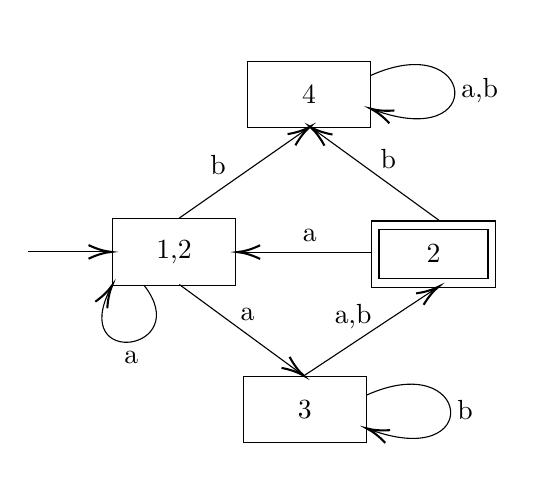
\begin{tikzpicture}[x=0.75pt,y=0.75pt,yscale=-1,xscale=1]
		%uncomment if require: \path (0,293.79998779296875); %set diagram left start at 0, and has height of 293.79998779296875
		
		%Shape: Rectangle [id:dp1427592945615206] 
		\draw   (246,107) -- (305.5,107) -- (305.5,138.91) -- (246,138.91) -- cycle ;
		%Straight Lines [id:da38177399363081044] 
		\draw    (205.5,122.91) -- (243.5,122.91) ;
		\draw [shift={(245.5,122.91)}, rotate = 180] [color={rgb, 255:red, 0; green, 0; blue, 0 }  ][line width=0.75]    (10.93,-3.29) .. controls (6.95,-1.4) and (3.31,-0.3) .. (0,0) .. controls (3.31,0.3) and (6.95,1.4) .. (10.93,3.29)   ;
		
		%Shape: Rectangle [id:dp8773457583333093] 
		\draw   (374.5,112) -- (427,112) -- (427,135.91) -- (374.5,135.91) -- cycle ;
		%Curve Lines [id:da18454774381199335] 
		\draw    (368.5,191.91) .. controls (418.99,169.14) and (425.38,228.69) .. (370.19,208.54) ;
		\draw [shift={(368.5,207.91)}, rotate = 381.1] [color={rgb, 255:red, 0; green, 0; blue, 0 }  ][line width=0.75]    (10.93,-3.29) .. controls (6.95,-1.4) and (3.31,-0.3) .. (0,0) .. controls (3.31,0.3) and (6.95,1.4) .. (10.93,3.29)   ;
		
		%Shape: Rectangle [id:dp8938638174206204] 
		\draw   (309,183) -- (368.5,183) -- (368.5,214.91) -- (309,214.91) -- cycle ;
		%Shape: Rectangle [id:dp6637696484220612] 
		\draw   (371,108) -- (430.5,108) -- (430.5,139.91) -- (371,139.91) -- cycle ;
		%Shape: Rectangle [id:dp24294652473658607] 
		\draw   (311,31) -- (370.5,31) -- (370.5,62.91) -- (311,62.91) -- cycle ;
		%Straight Lines [id:da4640110088822882] 
		\draw    (278.3,138.6) -- (336.69,181.42) ;
		\draw [shift={(338.3,182.6)}, rotate = 216.25] [color={rgb, 255:red, 0; green, 0; blue, 0 }  ][line width=0.75]    (10.93,-3.29) .. controls (6.95,-1.4) and (3.31,-0.3) .. (0,0) .. controls (3.31,0.3) and (6.95,1.4) .. (10.93,3.29)   ;
		
		%Straight Lines [id:da7179800592836478] 
		\draw    (338.3,182.6) -- (401.63,140.7) ;
		\draw [shift={(403.3,139.6)}, rotate = 506.51] [color={rgb, 255:red, 0; green, 0; blue, 0 }  ][line width=0.75]    (10.93,-3.29) .. controls (6.95,-1.4) and (3.31,-0.3) .. (0,0) .. controls (3.31,0.3) and (6.95,1.4) .. (10.93,3.29)   ;
		
		%Straight Lines [id:da4833983237746382] 
		\draw    (278.3,106.6) -- (339.66,63.75) ;
		\draw [shift={(341.3,62.6)}, rotate = 505.07] [color={rgb, 255:red, 0; green, 0; blue, 0 }  ][line width=0.75]    (10.93,-3.29) .. controls (6.95,-1.4) and (3.31,-0.3) .. (0,0) .. controls (3.31,0.3) and (6.95,1.4) .. (10.93,3.29)   ;
		
		%Straight Lines [id:da319416367590172] 
		\draw    (342.92,63.77) -- (403.3,107.6) ;
		
		\draw [shift={(341.3,62.6)}, rotate = 35.97] [color={rgb, 255:red, 0; green, 0; blue, 0 }  ][line width=0.75]    (10.93,-3.29) .. controls (6.95,-1.4) and (3.31,-0.3) .. (0,0) .. controls (3.31,0.3) and (6.95,1.4) .. (10.93,3.29)   ;
		%Curve Lines [id:da6696030147212659] 
		\draw    (370.5,37.91) .. controls (420.99,15.14) and (427.38,74.69) .. (372.19,54.54) ;
		\draw [shift={(370.5,53.91)}, rotate = 381.1] [color={rgb, 255:red, 0; green, 0; blue, 0 }  ][line width=0.75]    (10.93,-3.29) .. controls (6.95,-1.4) and (3.31,-0.3) .. (0,0) .. controls (3.31,0.3) and (6.95,1.4) .. (10.93,3.29)   ;
		
		%Curve Lines [id:da5652823058400562] 
		\draw    (261.3,139) .. controls (286.05,170.68) and (224.55,179.82) .. (245.34,140.12) ;
		\draw [shift={(246,138.91)}, rotate = 478.92] [color={rgb, 255:red, 0; green, 0; blue, 0 }  ][line width=0.75]    (10.93,-3.29) .. controls (6.95,-1.4) and (3.31,-0.3) .. (0,0) .. controls (3.31,0.3) and (6.95,1.4) .. (10.93,3.29)   ;
		
		%Straight Lines [id:da888273677844096] 
		\draw    (371.3,123) -- (308.3,123) ;
		\draw [shift={(306.3,123)}, rotate = 360] [color={rgb, 255:red, 0; green, 0; blue, 0 }  ][line width=0.75]    (10.93,-3.29) .. controls (6.95,-1.4) and (3.31,-0.3) .. (0,0) .. controls (3.31,0.3) and (6.95,1.4) .. (10.93,3.29)   ;
		
		% Text Node
		\draw (275.75,122.95) node  [align=left] {1,2};
		% Text Node
		\draw (416,199) node  [align=left] {b};
		% Text Node
		\draw (338.75,198.95) node  [align=left] {3};
		% Text Node
		\draw (400.75,123.95) node  [align=left] {2};
		% Text Node
		\draw (340.75,46.95) node  [align=left] {4};
		% Text Node
		\draw (423,45) node  [align=left] {a,b};
		% Text Node
		\draw (255,174) node  [align=left] {a};
		% Text Node
		\draw (311,153) node  [align=left] {a};
		% Text Node
		\draw (379,78) node  [align=left] {b};
		% Text Node
		\draw (341,115) node  [align=left] {a};
		% Text Node
		\draw (297,81) node  [align=left] {b};
		% Text Node
		\draw (362,154) node  [align=left] {a,b};
		
		\end{tikzpicture}
\end{enumerate}

\begin{problem}{1.17}
\end{problem}
\begin{enumerate}
	\item[(a)]
		$\{ \: \{\varepsilon, 0, 01, 010, 00, 001\}, \{0, 1\}, \delta, \varepsilon, \{\varepsilon, 01, 010, 001\}\}$	\\
		$\delta = 
		\begin{array}{ c|c|c|c }
			 & 0 & 1 & \varepsilon\\
			\hline
			\varepsilon & 0 & - & \varepsilon\\
			\hline
			0 & 00 & 01 & 0\\
			\hline
			01 & 010,\ 0 & - & \varepsilon,01\\
			\hline
			010 & 0 & - & \varepsilon,\ 010\\
			\hline
			00 & - & 001 & 00\\
			\hline
			001 & 0 & - & \varepsilon,\ 001
		\end{array}$\\
	\item[(b)]
		$\{ \: \{\varepsilon, 0, 01, 010, 00, 001, end\}, \{0, 1\}, \delta, \varepsilon, \{\varepsilon, 01, 010, 001\}\}$	\\
		$\delta = 
		\begin{array}{ c|c|c }
			 & 0 & 1\\
			\hline
			\varepsilon & 0 & end\\
			\hline
			0 & 00 & 01\\
			\hline
			01 & 010 & end\\
			\hline
			010 & 0 & 01\\
			\hline
			00 & end & 001\\
			\hline
			001 & 0 & end\\
			\hline
			end & end & end
		\end{array}$\\

\end{enumerate}


\begin{problem}{1.18}
\end{problem}
\begin{enumerate}
	\item[(a)]
		$1\Sigma^*0$
	\item[(b)]
		$\Sigma^*1\Sigma^*1\Sigma^*1\Sigma^*$
	\item[(c)]
		$\Sigma^*0101\Sigma^*$
	\item[(d)]
		$\Sigma\Sigma0\Sigma^*$
	\item[(e)]
		$0(\Sigma\Sigma)^*\cup1\Sigma(\Sigma\Sigma)^*$
	\item[(f)]
		$1?(0^+1?)^*1?\cup1^*$
	\item[(g)]
		$\Sigma?\Sigma?\Sigma?\Sigma?\Sigma?$
	\item[(h)]
		$\Sigma^4\Sigma^*\cup\Sigma?\cup0\Sigma\Sigma\cup\Sigma0\Sigma\cup\Sigma\Sigma0$
	\item[(i)]
		$(1\Sigma)^*1?$
	\item[(j)]
		$00^+1?\cup1?00^+\cup0^+1?0^+$
	\item[(k)]
		$\varepsilon\cup0$
	\item[(l)]
		$(1^*01^*01^*)^*\cup0^*10^*10^*$
	\item[(m)]
		$\varepsilon$
	\item[(n)]
		$\Sigma^+$
\end{enumerate}

\begin{problem}{1.20}
\end{problem}
\begin{enumerate}
	\item[(a)]
		Member: $a, b$\\
		Not member: $ba, bbaa$
	\item[(b)]
		Member: $ab, abab$\\
		Not member: $ba, aa$
	\item[(c)]
		Member: $a, b$\\
		Not member: $ab, ba$
	\item[(d)]
		Member: $\varepsilon, aaa$\\
		Not member: $b, bb$
	\item[(e)]
		Member: $aba, abaa$\\
		Not member: $a, b$
	\item[(f)]
		Member: $aba, bab$\\
		Not member: $a, b$
	\item[(g)]
		Member: $ab, b$\\
		Not member: $a, aa$
	\item[(h)]
		Member: $a, ba$\\
		Not member: $b, \varepsilon$
\end{enumerate}


\begin{problem}{1.21}
\end{problem}
\begin{enumerate}
	\item[(a)]
		$a^*b(a^*ba^*ba^*)^*$
	\item[(b)]
		$(\Sigma a^*b(bb)^*a)^*\cup\Sigma a^*b((bb)^*a\Sigma a^*b(bb)^*)^*$
\end{enumerate}

\begin{problem}{1.22}
\end{problem}
\begin{enumerate}
	\item[(a)]
		$\{ \:\{\varepsilon, q0, q1, a, b, q2, q3, -\}, \{/, \#, a, b\}, \delta, \varepsilon, \{q3\}\}$	\\
		$\delta = 
		\begin{array}{ c|c|c|c|c }
			 & / & \# & a & b\\
			\hline
			\varepsilon  & q0 & - & - & -\\
			\hline
			q0 & - & q1 & - & -\\
			\hline
			q1 & - & - & a & b\\
			\hline
			a & - & q2 & a & b\\
			\hline
			b & - & q2 & a & b\\
			\hline
			q2 & q3 & - & - & -\\
			\hline
			q3 & - & - & - & -\\
			\hline
			- & - & - & - & -
		\end{array}$\\
		
	\item[(b)]
		$/\#(a?b?)^*\#/$
\end{enumerate}

\end{document}